%%%%%%%%%%%%%%%%%%%%%%%%%%%%%%%%%%%%%%%%%%%%%%%%%%%%%%%%%%%%%%
%% Master Thesis
%% Learning-Based Online Adaptation for Control of a
%% Hydraulic Manipulator
%%
%% main file: main.tex
%% Template: RRLab rrlab.cls (RPTU Kaiserslautern-Landau)
%%%%%%%%%%%%%%%%%%%%%%%%%%%%%%%%%%%%%%%%%%%%%%%%%%%%%%%%%%%%%%

\documentclass[thesis,en,openany]{template/rrlab}

%%%%%%%%%%%%%%%%%%%%%%%%%%%%%%%%%%%%%%%%%%%%%%%%%%%%%%%%%%%%
%% Mandatory information
%%%%%%%%%%%%%%%%%%%%%%%%%%%%%%%%%%%%%%%%%%%%%%%%%%%%%%%%%%%%

% Title of the work:
\RRLABtitle{Learning-Based Online Adaptation for Control of a Hydraulic Manipulator}

% Author of the work:
\RRLABauthor{Kevin Kudakwashe Murera}

% Type of the work:
\RRLABtype{Master Thesis}

% Date of issue
\RRLABinception{23 March 2026}

% Date of submission
\RRLABsubmission{\today}

% First reviewer
\RRLABfirstreviewer{Prof. Dr. Karsten Berns}

% Supervisor
\RRLABsupervisor{M.Sc. Qi Li}

%%%%%%%%%%%%%%%%%%%%%%%%%%%%%%%%%%%%%%%%%%%%%%%%%%%%%%%%%%%%
%% Additional packages and own macros
%%%%%%%%%%%%%%%%%%%%%%%%%%%%%%%%%%%%%%%%%%%%%%%%%%%%%%%%%%%%
%%%%%%%%%%%%%%%%%%%%%%%%%%%%%%%%%%%%%%%%%%%%%%%%%%%%%%%%%%%%
%% Additional packages
%%
%% Already loaded by rrlab.cls — do NOT load again:
%%   graphicx, booktabs, xcolor, listings, longtable, fancyhdr,
%%   amssymb, amsmath, dsfont, hyperref, caption, subcaption
%%   (use \begin{subfigure} from subcaption, NOT the subfig package),
%%   units (incompatible with siunitx — use \unit{...} instead)
%%%%%%%%%%%%%%%%%%%%%%%%%%%%%%%%%%%%%%%%%%%%%%%%%%%%%%%%%%%%
\usepackage{algorithm2e}
\usepackage{multirow}
\usepackage{bm}

% Block diagrams
\usepackage{tikz}
\usetikzlibrary{arrows.meta,positioning,calc,fit,backgrounds,shapes.geometric}

% Colorblind-safe accent colors (Okabe-Ito), shared with the plots
\definecolor{cbblue}{RGB}{0,114,178}
\definecolor{cborange}{RGB}{230,159,0}
\definecolor{cbgreen}{RGB}{0,158,115}
\definecolor{cbpink}{RGB}{204,121,167}

\tikzset{
  sigblock/.style={draw=black!70, rounded corners=2pt, fill=cbblue!8,
    minimum height=8.5mm, minimum width=20mm, align=center, font=\small,
    inner sep=2.5pt},
  netblock/.style={sigblock, fill=cbblue!15},
  physblock/.style={sigblock, fill=cbgreen!12},
  datablock/.style={sigblock, fill=cborange!15},
  plantblock/.style={sigblock, fill=black!8},
  siglabel/.style={font=\scriptsize, align=center},
  sigarrow/.style={-{Latex[length=2.2mm]}, semithick},
}

%%%%%%%%%%%%%%%%%%%%%%%%%%%%%%%%%%%%%%%%%%%%%%%%%%%%%%%%%%%%
%% Own macros
%%%%%%%%%%%%%%%%%%%%%%%%%%%%%%%%%%%%%%%%%%%%%%%%%%%%%%%%%%%%

% Nomenclature shorthands (q, q-dot, cylinder extension/velocity,
% differential pressure, valve command, latent vector, PPO action)
\newcommand{\jointpos}{\ensuremath{\mathbf{q}}}
\newcommand{\jointvel}{\ensuremath{\dot{\mathbf{q}}}}
\newcommand{\cylext}{\ensuremath{\mathbf{s}}}
\newcommand{\cylvel}{\ensuremath{\dot{\mathbf{s}}}}
\newcommand{\dpress}{\ensuremath{\Delta p}}
\newcommand{\valvecmd}{\ensuremath{\mathbf{u}}}
\newcommand{\latent}{\ensuremath{\mathbf{z}}}
\newcommand{\ppoaction}{\ensuremath{\mathbf{a}}}

% Model / method abbreviations
\newcommand{\ID}{ID}
\newcommand{\FD}{FD}
\newcommand{\ROM}{ROM}
\newcommand{\SD}{SD}
\newcommand{\AAM}{AAM}
\newcommand{\DLS}{DLS}
\newcommand{\PPO}{PPO}

% Concise labels for the three control stacks. Their full PPO names are
% defined once in Chapter 1; the short labels are used thereafter.
\newcommand{\ppoROM}{\mbox{R}}
\newcommand{\ppoIDFD}{\mbox{IF}}
\newcommand{\ppoAAMIDFD}{\mbox{AIF}}

% Privileged factor vector, privileged latent, deployable latent estimate.
\newcommand{\factorvec}{\ensuremath{\mathbf{e}}}
\newcommand{\latenthat}{\ensuremath{\hat{\mathbf{z}}}}

% TODO marker visible in the draft
\newcommand{\todo}[1]{\textbf{[TODO: #1]}}

% Boxed research statement, used once in Section~\ref{sec:intro:contributions}.
\newcommand{\researchstatement}[1]{%
  \begin{center}
  \begin{tikzpicture}
    \node[draw=red!65!black, fill=red!3, rounded corners=5pt, line width=1pt,
          inner sep=11pt, text width=.86\linewidth, align=center]
      {\itshape #1};
  \end{tikzpicture}
  \end{center}}


\begin{document}

%%%%%%%%%%%%%%%%%%%%%%%%%%%%%%%%%%%%%%%%%%%%%%%%%%%%%%%%%%%%
%% Front matter
%%%%%%%%%%%%%%%%%%%%%%%%%%%%%%%%%%%%%%%%%%%%%%%%%%%%%%%%%%%%

% Title page (optional middle content, e.g. an image, and the date)
\RRLABtitlepage{}{\RRLABVARsubmission}

% Second page with title, author, supervisor etc.
\RRLABsecondpage

% Declaration of academic integrity (parameter: signing date)
\RRLABdeclaration{\today}

% Acknowledgements (optional)
\RRLABpreface{Acknowledgements}{%
I would like to express my sincere gratitude to my supervisor,
\textbf{Mr. Qi Li}, for their invaluable guidance, support, and
encouragement throughout this Master's thesis.

I am grateful to \textbf{Professor Dr. Karsten Berns} for providing the resources
of the Robotics Research Lab, without which the experimental work in this
thesis would not have been possible.

I am also deeply grateful to my family for their unwavering love and belief in
me, and to my friends for their support and encouragement throughout this
journey.

I sincerely thank everyone who contributed, directly or indirectly, to making
this achievement possible.
}

% Abstract (~250--400 words: problem, approach, datasets, the three
% stacks R / IF / AF, principal results,
% contribution. State results according to completed evidence.)
\RRLABabstract{Abstract}{%
Hydraulic manipulators are difficult to control accurately because actuator
response is nonlinear and changes with load, supply pressure and machine
condition. High-fidelity hydraulic simulation captures these effects but is too
slow for large-scale reinforcement learning, whereas direct joint control omits
the actuator behaviour that governs deployment performance. This thesis
investigates how learned hydraulic dynamics can be transferred into efficient
robot simulation, used for reinforcement-learning control and extended with
online adaptation on a verge-mowing manipulator.

Two actuator representations are identified from the same Simscape data: a
modular inverse--forward chain and a structurally constrained,
command-conditioned reduced-order model. Open-loop excitation and command
ablation test whether each model responds to the valve input, since low
prediction error alone can conceal a model that merely extrapolates smooth
state trajectories. The models are embedded in GPU-parallel PhysX training. A
classical controller supplies privileged demonstrations during training, then a
distilled policy replaces it completely at deployment. Evaluation covers held-out
meshes, eleven trajectory families and sixteen reserved plant configurations.

Both actuator representations support closed-loop control but produce different
trade-offs. Across $33$ matched evaluation cells, the inverse--forward chain has
$9.3$\,mm lower median lateral error, whereas the reduced-order model has
$1.7$\,mm lower median cut-height error; neither mean difference is resolved.
Online adaptation extends a frozen direct-valve actor with four context columns
driven by a payload estimate inferred from its existing $66$-channel
observation. At four and five times nominal payload on held-out mesh 3141,
adaptation reduces median cut-height error by $71.5$ and $82.2$\,mm, reduces
lateral error by $71.6$ and $107.1$\,mm, and increases ground contact by $0.12$
and $0.09$, respectively. Every pooled confidence interval excludes zero, and
the effects repeat on a second reserved mesh. At three times nominal payload,
where the frozen controller still maintains contact, conditioning instead
worsens lateral accuracy. Correct payload estimates outperform permuted ones,
although plausible but mispaired loads recover most of the gain.

The results show that prediction accuracy must be accompanied by a test of
control authority, actuator representation changes the learned controller, and
online adaptation is useful when a control-relevant robustness deficit remains
and the correction retains authority.
}

% Table of contents
\RRLABcontents

%%%%%%%%%%%%%%%%%%%%%%%%%%%%%%%%%%%%%%%%%%%%%%%%%%%%%%%%%%%%
%% Main matter - one file per chapter
%%%%%%%%%%%%%%%%%%%%%%%%%%%%%%%%%%%%%%%%%%%%%%%%%%%%%%%%%%%%

% Insert exactly one unnumbered, header-free blank page between chapters.
% The openany class option prevents the book class from adding a second
% parity-dependent blank page at the following chapter opening.
\newcommand{\RRLABchapterblank}{%
  \clearpage
  \begingroup
    \thispagestyle{empty}%
    \mbox{}%
    \clearpage
  \endgroup}

% Preserve the template's normal paragraph and heading gaps.  With
% \flushbottom, pages containing fixed figures or algorithms stretch those
% gaps to fill the text height, producing conspicuous empty bands mid-page.
\raggedbottom

%%%%%%%%%%%%%%%%%%%%%%%%%%%%%%%%%%%%%%%%%%%%%%%%%%%%%%%%%%%%
%% Chapter 1 - Introduction (indicative length: 6-9 pages)
%% Purpose: introduce the practical and scientific problem,
%% motivate the proposed learning-based adaptive architecture,
%% and state exactly what the thesis contributes.
%% Main output: research problem, research questions,
%% objectives, contributions, scope, and chapter roadmap.
%%%%%%%%%%%%%%%%%%%%%%%%%%%%%%%%%%%%%%%%%%%%%%%%%%%%%%%%%%%%
\chapter{Introduction}
\label{chap:introduction}

\section{The Role of Mechanised Verge Maintenance}
\label{sec:intro:verge}

Road verges are cut because they are infrastructure. Vegetation left to grow
closes sight lines at junctions and bends, obscures signs and barriers, blocks
the drainage channels that keep water off the carriageway, and encroaches on the
running surface itself. A national road network carries tens of thousands of
kilometres of verge, and each kilometre is cut several times in a growing
season, so the work is continuous, repetitive and performed almost entirely by
machine.

It is also performed from a moving vehicle. Stopping to cut each section would
require closing the lane, so a carrier drives the road at a few kilometres per
hour while a boom-mounted mowing head works the verge alongside it. The head
must hold a cut height of a few centimetres over ground that rises and falls
continuously, follow a grass line that curves with the road, and do so without
striking the surface hard enough to damage the tool or lift the machine.

The demands on the manipulator follow from that. The machine studied here,
shown in Figure~\ref{fig:intro:fme500}, carries a heavy rotating tool at the end
of a long boom, works in intermittent contact with the ground,
and must place that tool accurately while its own base is in motion. Hydraulic
actuation is the standard answer at this scale: it supplies the force density
and the tolerance to shock loading that electric drives do not, and it does so
with components rugged enough for continuous outdoor operation. Precision,
however, is not what hydraulics are good at, and that tension is the subject of
this thesis.

\section{Advances in Learning-Based Control for Hydraulic Manipulators}
\label{sec:intro:advances}

Two developments have changed what is achievable on machines of this kind.

The first is that policy optimisation in simulation has become practical for
contact-rich manipulation. GPU-parallel physics engines run thousands of
environments simultaneously, which makes reinforcement learning feasible on
tasks that would take years of real-machine experience, and randomising the
simulator across a family of plants produces policies that transfer without
being tuned to one machine. The second is that the actuator itself can be
learned. Rather than deriving valve and cylinder behaviour from first principles
and fitting its parameters, a network trained on recorded motion can represent
the command-to-motion relationship directly, including the nonlinearities that
analytical models approximate away. Chapter~\ref{chap:fundamentals} sets out
both lines and the work they rest on.

Combining the two is attractive and not straightforward. A learned actuator
model must be cheap enough to evaluate inside the training loop, which rules out
the high-fidelity models used for offline analysis, and it must remain valid
across the family of machines the policy will meet. This has motivated a line of
work in which a compact code describing the current plant is inferred from
recent interaction history and supplied to the controller, so that a single
policy can serve a family rather than a single
machine. Such methods report substantial gains in legged locomotion and in
manipulation, and they are the direct antecedent of the architecture examined
here.

\begin{figure}[H]
  \centering
  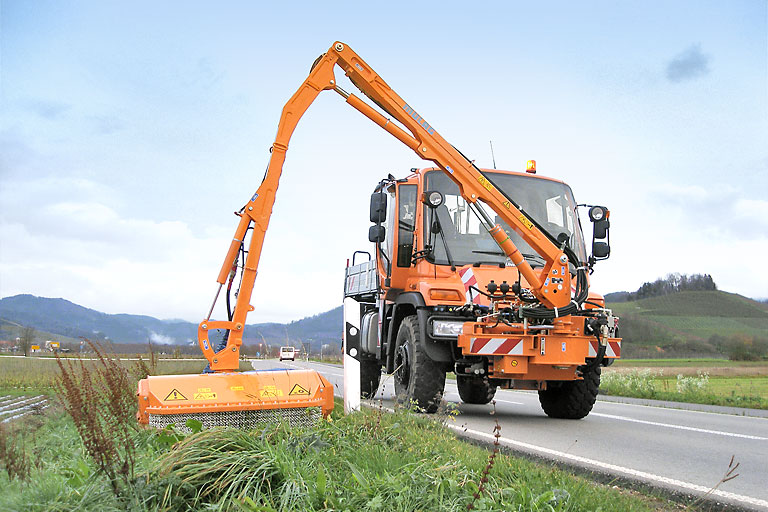
\includegraphics[width=.82\textwidth]{images/ch1/fme500_operation}
  \caption{MULAG FME~500 front mower on a Unimog during roadside verge
  maintenance. Image source: MULAG Fahrzeugwerk, FME~500 product
  documentation.}
  \label{fig:intro:fme500}
\end{figure}

\section{Challenges of Precise Tracking with Hydraulic Mowing Arms}
\label{sec:intro:challenges}

A valve command does not produce a proportional cylinder motion. The
relationship is nonlinear, depends on load and supply pressure, and is subject
to dead time between the command and any measurable response. It also differs
between machines: seal condition, fluid temperature, hose compliance and the
attachment fitted all change it, so two machines of the same model respond
differently and one machine responds differently across a season. A controller
that inverts only the geometry therefore leaves the largest source of tracking
error unaddressed.

That difficulty admits two responses, and they are routinely conflated. The
first is robustness: train across a randomised family so that a single fixed
model is adequate everywhere. It costs nothing at run time and gives up the
difference between the family and the individual. The second is adaptation:
infer which member of the family is present from the interaction history and
condition the model or the policy on that estimate. It promises to recover
that
difference, at the cost of an estimator that must work from observable signals
alone, since a deployed machine has no access to its own plant parameters.

Whether adaptation repays that cost depends on three things. Plant identity must
be present in the signals produced under the available excitation. The robust
controller must leave a control-relevant deficit to recover. The correction
path must retain enough authority to change the realised command. This thesis
measures these conditions on a hydraulic mowing arm and then evaluates whether
an online estimate of the operating condition improves closed-loop tracking.

\section{Contribution of This Thesis}
\label{sec:intro:contributions}

The difficulty described in Section~\ref{sec:intro:challenges} is a modelling
problem before it is a control problem. A hydraulic actuator can be simulated
accurately, but the models that do so are too slow to sit inside a
reinforcement-learning loop requiring millions of environment steps, while the
usual alternative of commanding joint positions directly removes the load and
pressure dependence that makes the machine difficult to control. What is needed
is a representation cheap enough to train against and faithful enough that the
resulting policy controls something close to the real actuator.

Learned actuator models and payload-conditioned adaptation are both established
techniques. What remains unclear is how such models should be identified so that
they retain the command dependence a controller needs, whether they transfer
between simulators without retraining, and what a controller must know about its
load once the models are used in control. Representation and transfer are
established first because the adaptation acts through an identified actuator
model rather than replacing one. Online adaptation is evaluated last so that any remaining
gain can be interpreted against the transferred model and the robustness of the
fixed controller. The order follows the dependencies among the claims. The
research statement is as follows:

\paragraph{Comparison notation.}
Three policy--actuator stacks are compared, each carrying a short label used
throughout. \emph{R} (\ppoROMfull) uses the command-conditioned reduced-order
model. \emph{IF} (\ppoIDFDfull) uses the frozen inverse and forward pair.
\emph{AF} (\ppoAAMFDfull) drops the inverse model and commands the valve
directly, which is where command authority remains. The labels name complete stacks rather than actuator models
alone, and Section~\ref{sec:ctrl:ppo-aamfd} gives their construction. One point
is worth fixing here because the name invites the opposite reading: the offline
AAM of Chapter~\ref{chap:models} is a diagnostic estimator and is not loaded in
the AF command path.

\researchstatement{To determine how hydraulic actuator dynamics learned from
high-fidelity simulation can be reduced, transferred into a computationally
efficient robotic simulation and used for reinforcement-learning control, and
under what conditions online adaptation improves on the robustness those learned
models already provide.}

The statement decomposes into six research questions, which are answered in the
order given. The first three concern how the actuator is represented, the fourth
concerns control through that representation, and the last two concern what
remains for adaptation once the first four are settled. The six questions are:

\begin{enumerate}
  \item How can data from a high-fidelity Simscape model be used to learn
    computationally tractable representations of hydraulic actuation while
    preserving the command dependence a controller requires?
  \item To what extent do actuator models identified from Simscape transfer to
    an IsaacLab manipulator without deployment-specific retraining?
  \item Can a structurally constrained reduced-order hydraulic model supply
    dynamics that are accurate and stable enough for GPU-parallel policy
    training?
  \item Can a policy trained from a privileged classical teacher become the sole
    deployed controller while acting through learned actuator dynamics?
  \item How does the choice of actuator representation affect tracking, command
    behaviour, latency and robustness under plant variation?
  \item Where plant variation survives robust training, can a controller
    estimate its own payload online and condition on it, and in which regime
    does that conditioning improve closed-loop tracking rather than cost it?
\end{enumerate}

RQ6 concerns one deployed mechanism. The policy receives a payload estimate
computed at runtime from the task observation it already carries, and only the
context columns of an otherwise frozen policy are trained, so zeroing the
estimate recovers the frozen controller exactly
(Section~\ref{sec:ctrl:af-residual}). What the policy is given is a single
physical quantity rather than an unconstrained code, and it is tested as such.
The AAM of Section~\ref{sec:models:aam} is not part of this path. It is an
offline diagnostic used to judge whether the inverse model can be trusted, and
the frozen stacks are robust controllers rather than adaptive ones.

The first question is answered in Chapters~\ref{chap:data}
and~\ref{chap:models}, the second and third in Chapter~\ref{chap:models}, the
fourth in Chapter~\ref{chap:control}, and the last two in
Chapter~\ref{chap:evaluation}.

RQ6 is the question named in the title and is deliberately placed last, since it
is only worth asking once the preceding questions have established that the
learned models transfer, that a policy can control through them, and how much
plant variation the closed loop already absorbs unaided. Its answer separates
two levels. Online plant context is usable at the model level, and whether that
benefit reaches the closed loop depends on the interface the correction acts
through: plant variation must remain control-relevant after robust training, be
observable from the available history, and reach a correction path with
sufficient authority. Any apparent gain must also be separated from the effect
of conditioning on a plausible load rather than the correct one. The work rests on the following contributions:

\textbf{Transferable Hydraulic Actuator Learning:} A pipeline that identifies
hydraulic actuation from high-fidelity Simscape data and transfers it into
IsaacLab through two representations, a modular inverse and forward chain and a
structurally constrained reduced-order model. The inverse and forward pair transfers
frozen, without deployment-specific retraining. The reduced-order model instead
receives a small bounded calibration against the deployment plant, so it serves
as a reference condition rather than an independent competitor
(Chapter~\ref{chap:models}).

\textbf{Control-Relevant Identification and Validation:} A demonstration that
predictive accuracy can conceal the loss of exactly the property a controller
needs, together with the procedure that detects it. A forward model reached a
near-perfect supervised score while learning to ignore the valve command. The
validation loss did not show this; ablating the command did. Excitation design
paired with input ablation is established here as a required test before a
learned actuator model is admitted to control
(Chapters~\ref{chap:data} and~\ref{chap:models}).

\textbf{Reduced-Order Actuator Model:} A command-conditioned recurrent actuator
surrogate whose transition is written as an explicit hydraulic chain, so the
predicted step stays differentiable in named quantities and bounded in form,
with learned heads covering valve realisation and unmodelled loading. It is
accurate enough to serve as the deployment plant, stable in recursive rollout,
and cheap enough to evaluate inside GPU-parallel policy training. It is not an
identified plant: the fitted physical constants settle on their clamps and the
realised motion comes from the learned heads, which is measured and reported
rather than assumed (Section~\ref{sec:models:rom}).

\textbf{Policy-Only Control Through Learned Hydraulics:} A damped least-squares
controller supplies privileged demonstrations during training and is then
removed, leaving the distilled policy as the entire deployed controller, acting
through learned actuator dynamics. Both representations support closed-loop
terrain following in that configuration
(Chapters~\ref{chap:control} and~\ref{chap:evaluation}). One training run
exists per representation, so this compares two realised controllers and does
not estimate what retraining either would produce.

\textbf{A Decision Procedure for Online Adaptation:} A matched protocol that
asks, in order, whether plant identity is present in the identification data,
what a privileged plant encoding does in the closed loop, and only then fits a
deployable estimator of it. Either of the first two measurements can show that a
correction would have nothing to act on
(Chapters~\ref{chap:models} and~\ref{chap:evaluation}).

\textbf{Where Online Adaptation Is Effective:} An online payload-conditioned
controller measured on one machine under one protocol, with the regime in which
it helps identified rather than assumed. It improves cut height, lateral
tracking and ground contact together where a heavy payload costs the frozen
controller ground contact, and costs lateral accuracy where the frozen
controller is not failing. Permuting the payload across environments separates
what correct identification contributes from what conditioning on any plausible
load contributes (Chapter~\ref{chap:evaluation}).

Chapter~\ref{chap:conclusion} restates these six with the measurements attached.
They are stated here as claims and there as results, so the evidence is given
once.

The causal plant estimator, the bounded adaptation path and the eight-gate
evaluation harness are described where they are used, as technical enablers
rather than separate claims.

Figure~\ref{fig:intro:research-cycle} condenses the logic that connects these
contributions. The sequence is a cycle rather than a one-way pipeline: evidence
from robustness, identifiability and adaptation feeds back into the next
actuator representation and the transfer assumptions made for it.

\begin{figure}[H]
  \centering
  \resizebox{.80\textwidth}{!}{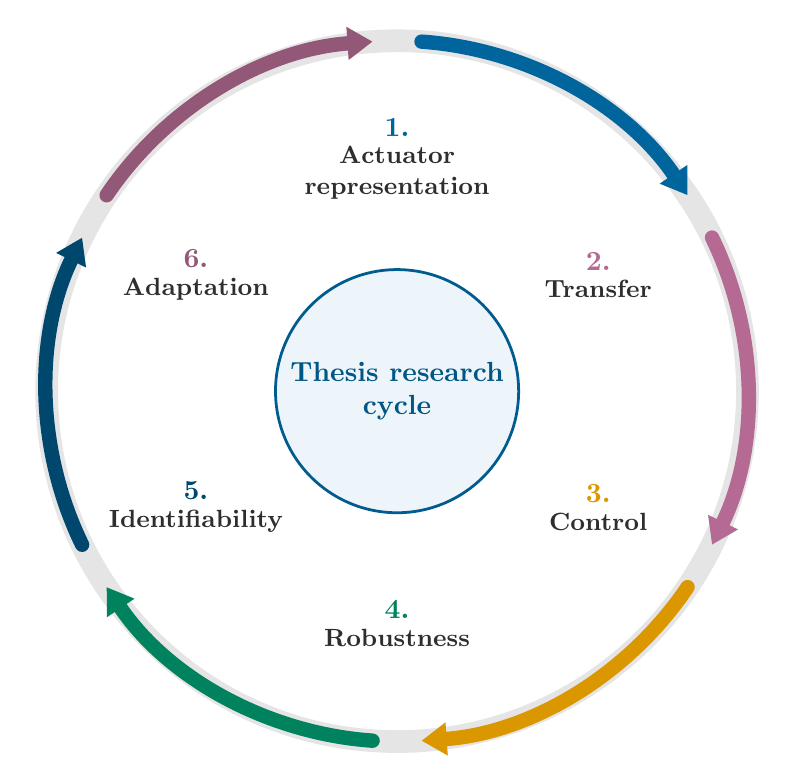
\begin{tikzpicture}[
  x=1cm,
  y=1cm,
  cyclearc/.style={-{Triangle[length=3.2mm,width=4.0mm]},
    line width=5.2pt,line cap=round},
  cyclelabel/.style={align=center,text width=2.90cm,
    font=\small\bfseries,text=black!82}
]
  % A pale uninterrupted track makes the circular structure explicit.
  \draw[draw=black!10,line width=8.2pt]
    (90:4.45) arc[start angle=90,end angle=-270,radius=4.45];

  % Six clockwise arcs form one closed cycle. Small gaps keep each arrowhead
  % distinct while the background track preserves continuity.
  \draw[cyclearc,draw=cbblue!88!black]
    (86:4.45) arc[start angle=86,end angle=34,radius=4.45];
  \draw[cyclearc,draw=cbpink!88!black]
    (26:4.45) arc[start angle=26,end angle=-26,radius=4.45];
  \draw[cyclearc,draw=cborange!95!black]
    (-34:4.45) arc[start angle=-34,end angle=-86,radius=4.45];
  \draw[cyclearc,draw=cbgreen!82!black]
    (-94:4.45) arc[start angle=-94,end angle=-146,radius=4.45];
  \draw[cyclearc,draw=cbblue!62!black]
    (-154:4.45) arc[start angle=-154,end angle=-206,radius=4.45];
  \draw[cyclearc,draw=cbpink!72!black]
    (-214:4.45) arc[start angle=-214,end angle=-266,radius=4.45];

  \node[cyclelabel] at (90:2.95)
    {\textcolor{cbblue!88!black}{\normalsize 1.}\\[-1pt]
     Actuator\\representation};
  \node[cyclelabel] at (30:2.95)
    {\textcolor{cbpink!88!black}{\normalsize 2.}\\[-1pt]Transfer};
  \node[cyclelabel] at (-30:2.95)
    {\textcolor{cborange!95!black}{\normalsize 3.}\\[-1pt]Control};
  \node[cyclelabel] at (-90:2.95)
    {\textcolor{cbgreen!82!black}{\normalsize 4.}\\[-1pt]Robustness};
  \node[cyclelabel] at (-150:2.95)
    {\textcolor{cbblue!62!black}{\normalsize 5.}\\[-1pt]Identifiability};
  \node[cyclelabel] at (150:2.95)
    {\textcolor{cbpink!72!black}{\normalsize 6.}\\[-1pt]Adaptation};

  \node[circle,draw=cbblue!80!black,line width=1pt,fill=cbblue!7,
    minimum size=2.65cm,align=center,font=\normalsize\bfseries,
    text=cbblue!75!black] at (0,0)
    {Thesis research\\cycle};
\end{tikzpicture}
}
  \caption{Research cycle connecting actuator representation, transfer,
  closed-loop control, robustness, identifiability, and adaptation. Evidence
  from the final stages informs the next actuator representation and its transfer
  assumptions.}
  \label{fig:intro:research-cycle}
\end{figure}

\section{Thesis Structure}
\label{sec:intro:structure}

This thesis investigates how hydraulic actuator dynamics learned from
high-fidelity simulation can be reduced, transferred into a computationally
efficient robotic simulation and used for reinforcement-learning control,
grounding that investigation in the identifiability of the actuator models and
in the robustness of the controllers built on them. The document is organised as
follows:

\textbf{Chapter~\ref{chap:fundamentals}} establishes the background against
which the remainder is read. It covers the actuation chain, the kinematic tools
underlying the classical controller, conventional model-based control of
hydraulic uncertainty, learned dynamics models and the pitfalls of identifying
them from closed-loop data, domain randomisation and latent adaptation. The
chapter closes by stating the gap that remains and where the three control
stacks sit against it.

\textbf{Chapter~\ref{chap:system}} analyses the platform, taking the MULAG
FME~500 on a Unimog carrier as the case study. It describes the rigid bodies and
the serial chain they form, the mappings between task space and cylinder space,
and the high-fidelity Simscape model the actuator data derives from. It also
fixes what the controller may observe and the evaluation gates every later
result is scored against.

\textbf{Chapter~\ref{chap:data}} presents the data generation strategy and
answers the first research question. It describes the excitation design, the
randomised factor set that defines the family of plants, and the procedures that
keep training, validation and reserved test configurations separate. It then
reports the identifiability audit, including the measured finding that
excitation gathered under a task controller does not separate plants and the
open-loop collection that repairs it.

\textbf{Chapter~\ref{chap:models}} develops the learned actuator models and
answers the next two research questions. It presents the inverse model, the
forward model, the evidence that supervised accuracy alone does not establish
command authority, and the reduced-order model that serves as the deployment
plant. It closes on the AAM as a diagnostic for whether the inverse model can be
trusted, and on the online payload estimator the deployed controller conditions
on.

\textbf{Chapter~\ref{chap:control}} describes the control framework and its
integration with the simulator, and answers the fourth research question. It
presents the damped least-squares teacher, the observation and action interfaces
the stacks hold in common, the distillation of the teacher into a student
policy, and the reference-anchored fine-tuning that keeps further optimisation
admissible. It then assembles the three deployed stacks and states which
comparison each one can carry.

\textbf{Chapter~\ref{chap:evaluation}} reports the experimental evaluation and
answers the last two research questions. It compares the matched pair on
tracking, command behaviour and dynamic response, and measures how much of the
randomised factor draw reaches each plant. It closes on online adaptation,
measured inside the adaptive stack against its own frozen base and a
permuted-payload control.

\textbf{Chapter~\ref{chap:conclusion}} concludes the thesis. It summarises what
the work establishes and what it does not, states the design implications that
follow, and records the limitations of the evidence. It ends with the future
work, which begins with the simulation experiments that would most change what
the thesis can claim and ends with transfer to the physical machine.

\RRLABchapterblank
%%%%%%%%%%%%%%%%%%%%%%%%%%%%%%%%%%%%%%%%%%%%%%%%%%%%%%%%%%%%
%% Chapter 2 - Fundamentals and Related Work (12-18 pages)
%% Purpose: provide only the theory and literature needed to
%% understand the research choices, then end with the
%% unresolved gap addressed by the thesis.
%%%%%%%%%%%%%%%%%%%%%%%%%%%%%%%%%%%%%%%%%%%%%%%%%%%%%%%%%%%%
\chapter{Fundamentals and Related Work}
\label{chap:fundamentals}

Chapter~\ref{chap:introduction} argued that precise task-space tracking
with a hydraulic mowing arm is limited less by kinematics than by the
actuator. The path from a valve command to actual cylinder motion is
nonlinear and load dependent, and it differs from one machine, season, or
attachment to the next. This chapter collects the background needed to
judge that argument and to understand the design decisions made later in
the thesis. Section~\ref{sec:fund:actuation} introduces the machine class
and its electro-hydraulic actuation. Section~\ref{sec:fund:kinematics}
recalls the kinematic tools behind the classical controller, and
Section~\ref{sec:fund:conventional-control} reviews how conventional
model-based control deals with hydraulic uncertainty. The remaining sections cover the learning methods this work builds on.
Section~\ref{sec:fund:learned-dynamics} treats data-driven dynamics models and
the pitfalls of identifying them from closed-loop data.
Section~\ref{sec:fund:rom} covers reduced-order and grey-box modelling,
Section~\ref{sec:fund:domain-randomization} domain randomisation and latent
adaptation, and Section~\ref{sec:fund:rl-residual} policy optimisation with
structured priors.
Section~\ref{sec:fund:gap} then states the gap that remains and how the
three control stacks of this thesis (\ppoROM, \ppoIDFD, and
\ppoAAMFD) address it. As defined in Chapter~\ref{chap:introduction},
the first two abbreviate PPO--ROM and PPO--ID--FD; AF denotes the deployed
Adaptive Forward stack rather than the offline AAM. Only material that is
needed for the later chapters is included. Background and results are kept
apart: where a later measurement is the reason a line of work was left behind,
it is quoted forward and marked as such, and no argument in this chapter rests
on it. The concrete system definition and problem formulation follow in
Chapter~\ref{chap:system}.

\section{Manipulator Actuation and Control Fundamentals}
\label{sec:fund:actuation}

\subsection{Application Context and Implement Carriers}

The MULAG FME~500 mounts a multi-link hydraulic boom and a
$\unit[1.2]{m}$ flail head on a Unimog carrier~\cite{mulag2026fme500}.
It reaches about $\unit[6.5]{m}$ laterally, below road level and over
obstacles, while an operator adjusts cutter height, tilt and lateral position
as the vehicle moves. Automating this continuous tracking task is the practical
motivation of the thesis.

Hydraulic cylinders suit the required force, shock tolerance and existing
vehicle power supply, but their command gain changes strongly with load and
configuration. This trade-off between force density and precision is central
to hydraulic manipulator control~\cite{mattila2017survey}.

\subsection{The Electro-Hydraulic Actuation Chain}
\label{sec:fund:actuation-chain}

\begin{figure}[H]
  \centering
  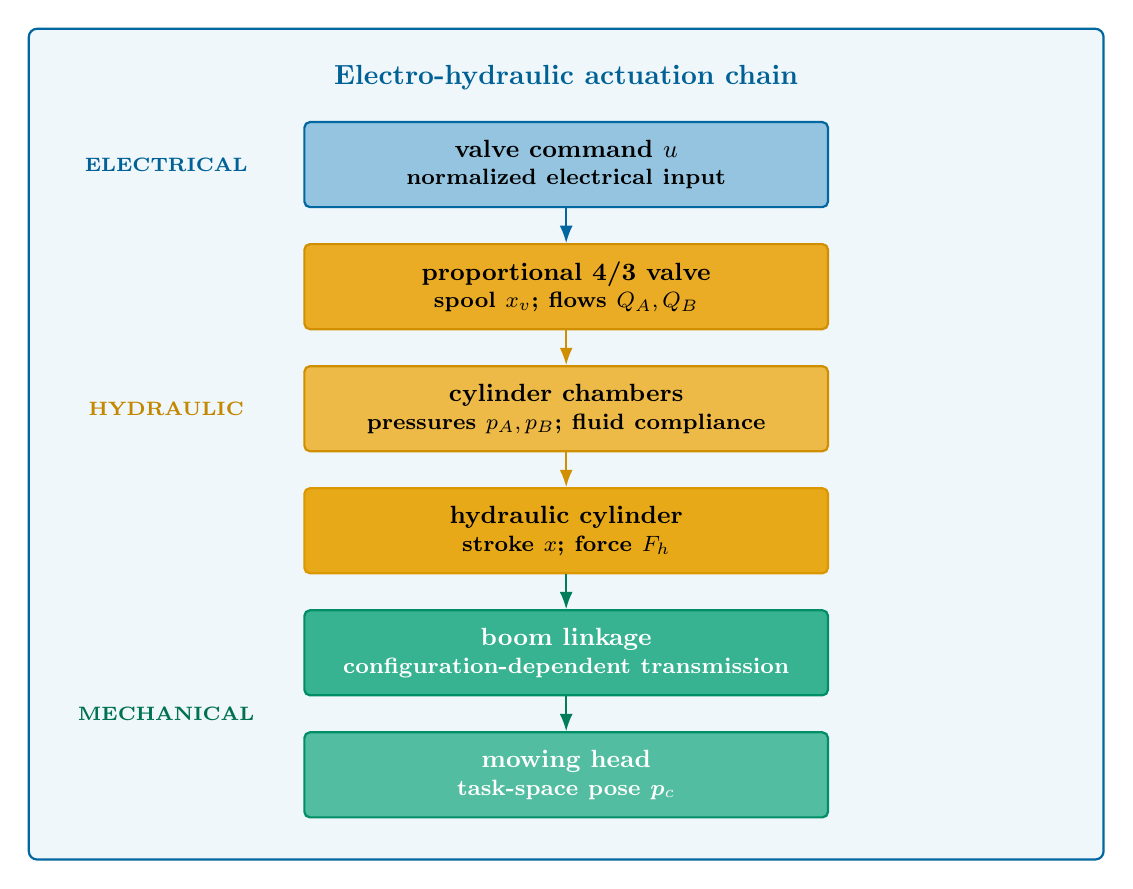
\begin{tikzpicture}[x=1cm,y=1cm,>=Latex,font=\small]
  % Match Figure 2.4: one pale framed panel, compact filled blocks and
  % unobstructed semantic-colour arrows.
  \node[draw=cbblue!90!black,line width=.8pt,rounded corners=3pt,
    fill=cbblue!6,minimum width=13.65cm,minimum height=10.55cm]
    (chainpanel) at (0,-4.55) {};
  \node[font=\normalsize\bfseries,text=cbblue!85!black] at (0,.10)
    {Electro-hydraulic actuation chain};

  \tikzset{
    chainblock/.style={draw=black!55,line width=.8pt,rounded corners=2pt,
      minimum width=6.65cm,minimum height=1.08cm,text width=6.15cm,
      align=center,font=\small\bfseries},
    groupname/.style={font=\scriptsize\bfseries,align=center}
  }

  \node[chainblock,draw=cbblue!90!black,fill=cbblue!42]
    (command) at (0,-1.00)
    {valve command $u$\\[-1pt]\footnotesize normalized electrical input};

  \node[chainblock,draw=cborange!90!black,fill=cborange!86]
    (valve) at (0,-2.55)
    {proportional 4/3 valve\\[-1pt]\footnotesize spool $x_v$; flows $Q_A,Q_B$};
  \node[chainblock,draw=cborange!90!black,fill=cborange!72]
    (chambers) at (0,-4.10)
    {cylinder chambers\\[-1pt]\footnotesize pressures $p_A,p_B$; fluid compliance};
  \node[chainblock,draw=cborange!95!black,fill=cborange!90]
    (cylinder) at (0,-5.65)
    {hydraulic cylinder\\[-1pt]\footnotesize stroke $x$; force $F_h$};

  \node[chainblock,draw=cbgreen!90!black,fill=cbgreen!78,text=white]
    (linkage) at (0,-7.20)
    {boom linkage\\[-1pt]\footnotesize configuration-dependent transmission};
  \node[chainblock,draw=cbgreen!90!black,fill=cbgreen!68,text=white]
    (head) at (0,-8.75)
    {mowing head\\[-1pt]\footnotesize task-space pose $\bm{p}_c$};

  \draw[sigarrow,cbblue!90!black] (command) -- (valve);
  \draw[sigarrow,cborange!90!black] (valve) -- (chambers);
  \draw[sigarrow,cborange!90!black] (chambers) -- (cylinder);
  \draw[sigarrow,cbgreen!80!black] (cylinder) -- (linkage);
  \draw[sigarrow,cbgreen!80!black] (linkage) -- (head);

  \node[groupname,text=cbblue!85!black] at (-5.08,-1.00) {ELECTRICAL};
  \node[groupname,text=cborange!85!black] at (-5.08,-4.10) {HYDRAULIC};
  \node[groupname,text=cbgreen!72!black] at (-5.08,-7.98) {MECHANICAL};
\end{tikzpicture}

  \caption{The electro-hydraulic actuation chain from valve command to
  mowing-head motion. The block colors distinguish the electrical, hydraulic
  and mechanical stages; each subtitle identifies the principal quantity
  passed to the next stage.}
  \label{fig:fund:chain}
\end{figure}

In Figure~\ref{fig:fund:chain}, an electrical command moves a proportional
valve spool and meters flow to the cylinder chambers. The orifice
law~\cite{merritt1967hydraulic} makes flow depend on spool position and the
square root of the pressure margin. Valve authority is therefore
load-dependent and directional; overlap creates a dead zone near null and the
spool saturates at large commands~\cite{jelali2003hydraulic}.

Compressibility, changing chamber volume, relief limits, leakage and seal
friction further separate flow from motion. Several of these effects are
non-smooth, while bulk modulus, leakage and friction drift with temperature and
wear. The mechanical linkage then converts cylinder translation through
configuration-dependent lever arms. Chapter~\ref{chap:models} consequently
models the hydraulic realisation in cylinder space, before kinematic effects
are mixed into cutter error.

\subsection{High-Fidelity Simulation as a Data Source}
\label{sec:fund:sim-data-source}

The component-level Simscape plant~\cite{mathworks2024simscape} resolves the
stiff hydraulic dynamics but runs one machine at small integration steps.
Policy optimisation instead benefits from thousands of GPU-parallel
plants~\cite{makoviychuk2021isaac}. The detailed model is therefore used
offline to generate identification data; compact actuator models carry its
behaviour into parallel training, as summarised in
Figure~\ref{fig:fund:simtosim}.

\begin{figure}[H]
  \centering
  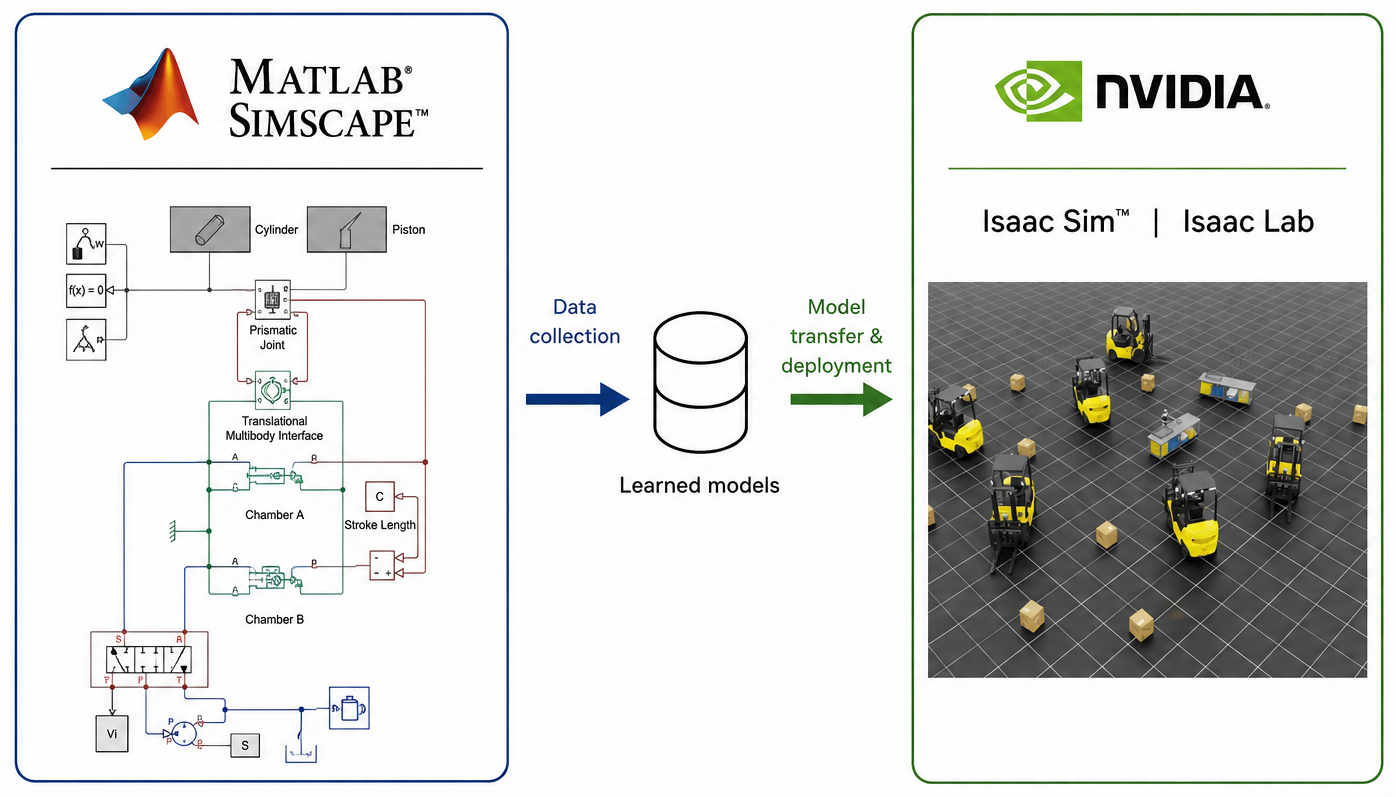
\includegraphics[width=\textwidth]{images/ch2/fund_sim_to_sim}
  \caption{Simscape supplies high-fidelity hydraulic data; compact actuator
  models transfer that behaviour to GPU-parallel training in IsaacLab. Product
  images: MathWorks and NVIDIA.}
  \label{fig:fund:simtosim}
\end{figure}

\section{Kinematics and Task-Space Tracking}
\label{sec:fund:kinematics}

\subsection{Differential Kinematics}

The cutter path is specified in vehicle coordinates, so the manipulator
Jacobian maps joint rates to the required tool velocity
~\cite{siciliano2009robotics}. Near singular configurations the ordinary
pseudo-inverse produces excessive commands. The damped least-squares inverse
of Wampler~\cite{wampler1986manipulator} and Nakamura and
Hanafusa~\cite{nakamura1986inverse} trades some local accuracy for bounded
commands and is retained as the classical controller.

\subsection{From Joint Space to Cylinder Space}

The actuated coordinates are cylinder lengths, and their nonlinear
cylinder-to-joint map has a configuration-dependent lever arm. A passive head
joint further limits independently controllable directions. The calibrated
cutter Jacobian in Chapter~\ref{chap:system} composes these mappings. It still
assumes that commanded cylinder motion is realised; the learned actuator models
address that remaining gap.

\section[Model-Based and Conventional Control Approaches]
  {Model-Based and Conventional Control\\Approaches}
\label{sec:fund:conventional-control}

Three families of conventional control are relevant here: fixed-gain cascades,
nonlinear cancellation, and online parameter estimation. Each of them works on
hydraulic manipulators. Each also carries a maintenance or excitation cost, and
those costs are the reason this thesis learns the actuator instead.

\subsection{Fixed-Gain Cascades}

Industrial implements commonly map joystick input directly to valve current.
The standard improvement is a cascade in which an outer position loop sets a
velocity or pressure reference and a fast inner loop tracks
it~\cite{jelali2003hydraulic}. The construction is cheap, needs no plant model
beyond a few tuned gains, and is what a commercial machine realistically ships
with.

The cost is that the gains are tuned around one operating point. The orifice
law makes command-to-velocity gain scale with the square root of the pressure
margin, so it changes with load and with direction of travel, and the linkage
lever arm changes with configuration. A gain set tuned at the stiff end of that
range responds weakly at the compliant end; tuned at the compliant end it
oscillates at the stiff end. Scheduling the gains over configuration and load
recovers some of the range, but the schedule is machine and attachment
specific and has to be remeasured whenever either changes.

\subsection{Nonlinear Cancellation}

Nonlinear model-based control removes the dependence on an operating point by
cancelling the known dynamics rather than tuning around
them~\cite{slotine1991applied}. For a hydraulic actuator the cancellation has
to span the orifice nonlinearity, chamber compressibility and the rigid-body
load, which places the valve command several integrations away from the
position error and makes backstepping the usual
construction~\cite{jelali2003hydraulic}. The survey of Mattila et
al.~\cite{mattila2017survey} reports this line, together with virtual
decomposition control, as the state of the art for heavy-duty hydraulic arms,
and it does deliver accurate tracking on instrumented machines.

Cancellation is only as good as the model it inverts, and the terms it depends
on are the terms that drift. Bulk modulus, leakage and seal friction change
with temperature and wear over a working day. Some of the structure is
non-smooth and cannot be cancelled at all: valve overlap produces a dead zone
that has to be inverted explicitly, as Yang et
al.~\cite{yang2026stateconstrained} do alongside state constraints. The learned
actuator models of Chapter~\ref{chap:models} carry an explicit dead-zone term
for the same reason. Maintaining this identification per machine, season and
attachment is what makes the family expensive on a commercial
implement~\cite{mattila2017survey}, not any weakness in the control law.

\subsection{Online Parameter Estimation}

Adaptive control estimates the uncertain parameters during operation instead of
fixing them in advance~\cite{astrom1995adaptive}. Yao's adaptive robust control
(ARC) pairs a projection-bounded parameter estimator with a robust feedback
term, so that a guaranteed transient tracking bound does not wait for the
estimate to converge, and it is the established result for single-rod
hydraulic actuators~\cite{yao2000adaptive}. On the face of it this is the
closest classical answer to the problem of this thesis, because it targets
exactly the drifting parameters just described, and because it is the one
classical family that ships a proof rather than an empirical trend, in direct
contrast to the adaptation studied here (Section~\ref{sec:ctrl:af-claims}). ARC
buys that guarantee by assuming a known parametric structure for the plant: the
orifice, chamber and friction terms must be derived correctly in advance, with
only their coefficients left uncertain. That is exactly the assumption
Chapter~\ref{chap:models} finds hard to hold on this machine, where the
reduced-order model's own orifice and friction parameters settle at their
optimisation clamps rather than at physically plausible values
(Section~\ref{sec:models:rom}).

Two properties of the task limit it. Parameter convergence requires persistent
excitation, and mowing supplies smooth, low-bandwidth commands that do not
provide it; the redundancy between command and state that
Section~\ref{sec:fund:identifiability} describes for learned models constrains
a recursive estimator in the same way. The valve also saturates for much of the
scored window on this machine (Section~\ref{sec:models:adapter}), where the
regressor stops reflecting the applied input and adaptation has to be suspended
or explicitly compensated~\cite{sofrony2024antiwindup}. Both limits belong to
the task rather than to the estimator, so they bear on any correction applied to
the command on this machine. They are measured
(Section~\ref{sec:models:adapter-null}) rather than assumed away, and they are
part of why the deployed mechanism conditions the policy instead of correcting
its command.

The scope of that argument should be stated plainly. No classical adaptive
baseline is run in this thesis. The experiments of
Chapter~\ref{chap:evaluation} compare actuator representations inside one
reinforcement-learning stack, so nothing here shows that adaptive robust
control tracks worse than the learned route on this machine. What is claimed is
narrower: the two conditions the classical estimator needs, informative
excitation and an unsaturated regressor, are not supplied by the mowing task,
and the maintenance burden the family carries per machine, season and
attachment is the burden the thesis is trying to remove.

The experiment that would settle the comparison is concrete rather than
hypothetical. It needs four things. The first is a per-cylinder
differential-pressure loop, because ARC's estimator is driven by the same
pressure signal this simulation only produces as an uncalibrated model state
(Appendix~\ref{app:pressure-signals}). The second is an open-loop
identification campaign on the physical implement, to fit the orifice and
friction structure ARC assumes rather than the clamped values the reduced-order
model settles on (Section~\ref{sec:models:rom}). The third is a projection bound
and adaptation gain tuned against that identified structure. The fourth is a
second control implementation, run on the same excitation schedule and
evaluation gates as Chapter~\ref{chap:evaluation}, so that the two families are
compared under one protocol rather than one against the literature's reported
numbers for the other. None of that instrumentation exists on the target machine
yet (Chapter~\ref{chap:conclusion}), which is why the comparison is left open
rather than run.

\subsection{What Is Retained}

The classical methods are not replaced wholesale. Kinematics is reliable and is
kept: the DLS controller of Section~\ref{sec:fund:kinematics} acts as teacher
and as the data-collection controller. What is learned is the part the
model-based families struggle to maintain: the mapping from cylinder command to
realised motion, and the policy that issues that command
(Section~\ref{sec:fund:rl-residual}).

\section{Data-Driven System Identification and Learned Dynamics}
\label{sec:fund:learned-dynamics}

\subsection{Learned Forward and Inverse Dynamics}

Robot model learning distinguishes forward models, which predict the next
state from state and command, from inverse models, which predict the command
for a desired transition~\cite{nguyentuong2011model}. Section
~\ref{sec:models:overview} fixes both interfaces. One-step fit is insufficient
when a forward model is recursively rolled out, because small errors compound
~\cite{nagabandi2018neural}. The models here are therefore trained with
multi-step objectives. Probabilistic ensembles represent growing rollout
uncertainty~\cite{chua2018deep}; recurrent architectures instead retain
unobserved pressure and valve history~\cite{hochreiter1997long,cho2014learning},
as used by the reduced-order model.

\subsection{Closed-Loop Identifiability}
\label{sec:fund:identifiability}

Informative identification requires inputs that excite the plant independently
of feedback~\cite{ljung1999system,isermann2011identification}. In closed-loop
data, command and state history are correlated; a flexible predictor can score
well by ignoring the command, and validation from the same distribution will
not reveal the shortcut~\cite{schoukens2019nonlinear}.

That failure occurred here: a closed-loop forward model reached one-step
$R^2\approx0.999$ yet showed almost no command dependence under ablation.
Chapter~\ref{chap:data} therefore uses open-loop valve excitation, and every
learned model is checked with zeroed and shuffled commands. Prediction score
alone is not treated as evidence of control authority.

\section{Reduced-Order Modelling}
\label{sec:fund:rom}

Reduced-order models retain dominant behaviour at lower cost
\cite{benner2015survey}. Here the full Simscape plant is reduced to
per-cylinder extension, velocity and pressure difference. The construction is
grey-box: known structure is embedded so that data fits what remains unknown
\cite{karniadakis2021physics}. As in the structured dynamics network of
Lutter et al. \cite{lutter2019deep}, explicit physical layers improve
interpretability. The hydraulic ROM retains the orifice, pressure and
integration structure; learned terms represent valve realisation,
configuration-dependent load and bounded residuals.

Hwangbo et al.~\cite{hwangbo2019learning} combined analytic rigid-body
mechanics with a learned actuator response, a pattern later scaled in
GPU-parallel simulation~\cite{rudin2022learning}. Yamamori et
al.~\cite{yamamori2026actuator} instead shaped the physical actuator to match
the simulation. A commercial valve and pump cannot be redesigned in that way,
so this thesis learns the hydraulic realisation while PhysX retains the
rigid-body mechanics (Figure~\ref{fig:fund:workflow}).

\begin{figure}[H]
  \centering
  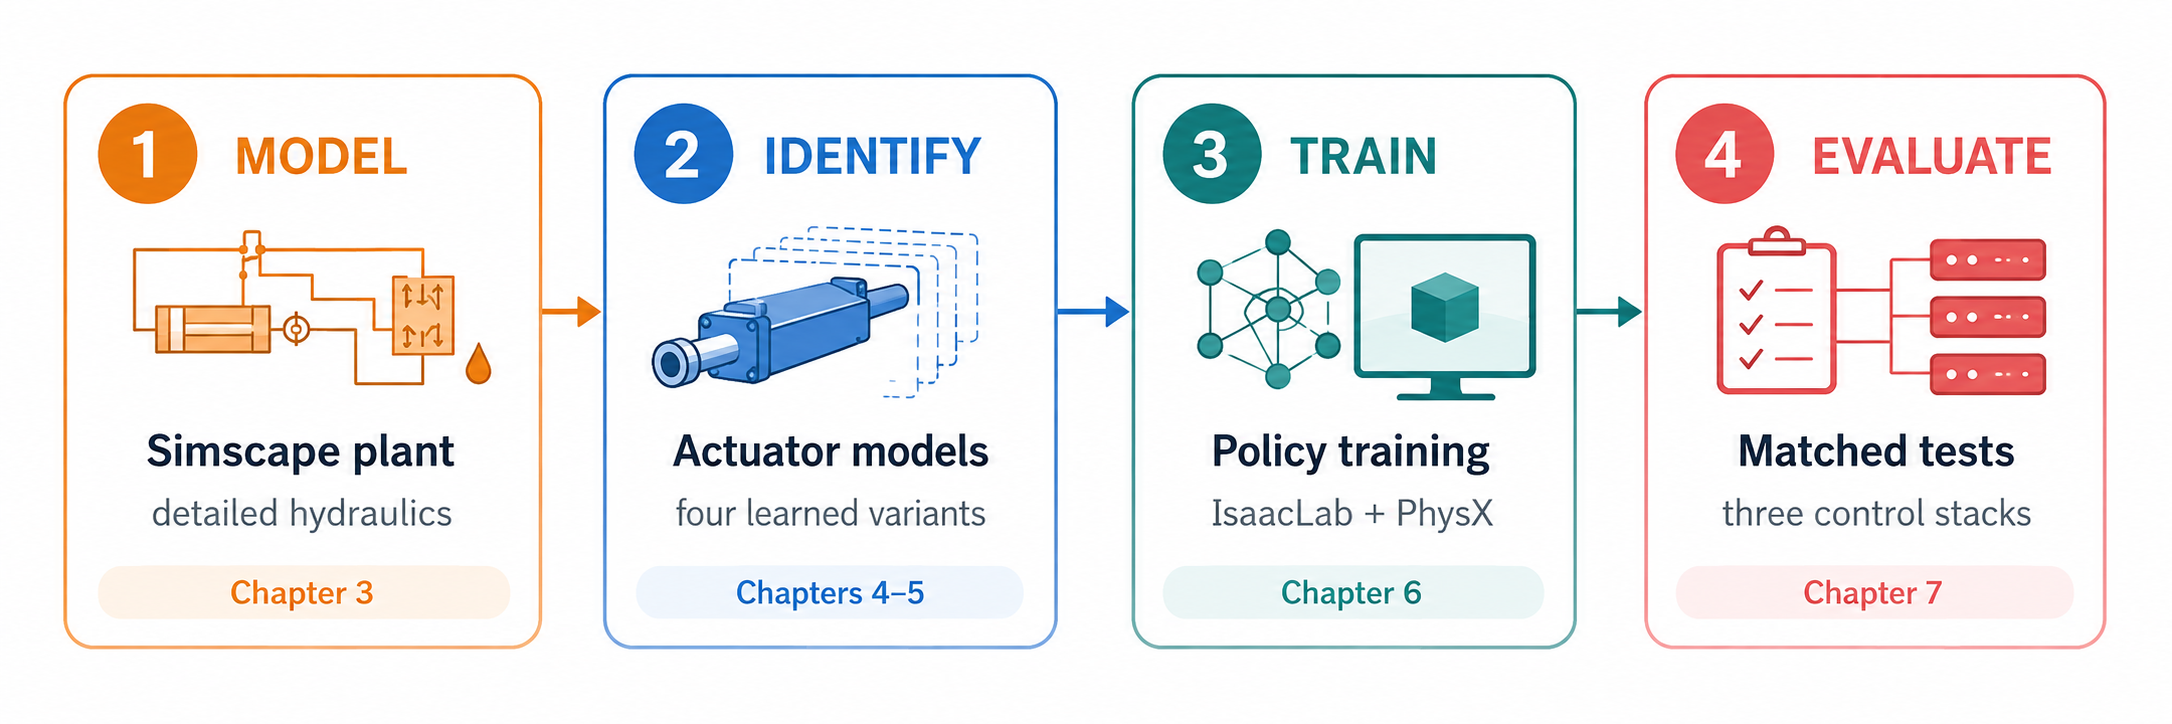
\includegraphics[width=\textwidth]{images/ch2/fund_workflow.png}
  \caption{Workflow from the hydraulic plant model to matched evaluation. The
  separation between rigid-body physics and learned actuation follows the
  actuator-network approach in~\cite{hwangbo2019learning}. This figure was
  generated using AI.}
  \label{fig:fund:workflow}
\end{figure}

\section{Domain Randomisation and Latent Adaptation}
\label{sec:fund:domain-randomization}

\subsection{Robustness Through Randomised Training}

A model trained on one simulated plant inherits its parameters as assumptions.
Domain randomisation instead trains across a family, first for visual
appearance~\cite{tobin2017domain} and then for dynamics such as mass,
friction, gain and latency~\cite{peng2018sim}. The hydraulic family in
Chapter~\ref{chap:data} varies bulk modulus, valve gain, leakage, friction and
payload, producing robustness to physically plausible plant variation.

\newpage
\subsection{From Robustness to Adaptation}
\label{sec:fund:adaptation}

Figure~\ref{fig:fund:robust-adaptive} contrasts a policy trained for one robust
response across the plant family with an adaptive stack that conditions its
response on the current plant.

\begin{figure}[H]
  \centering
  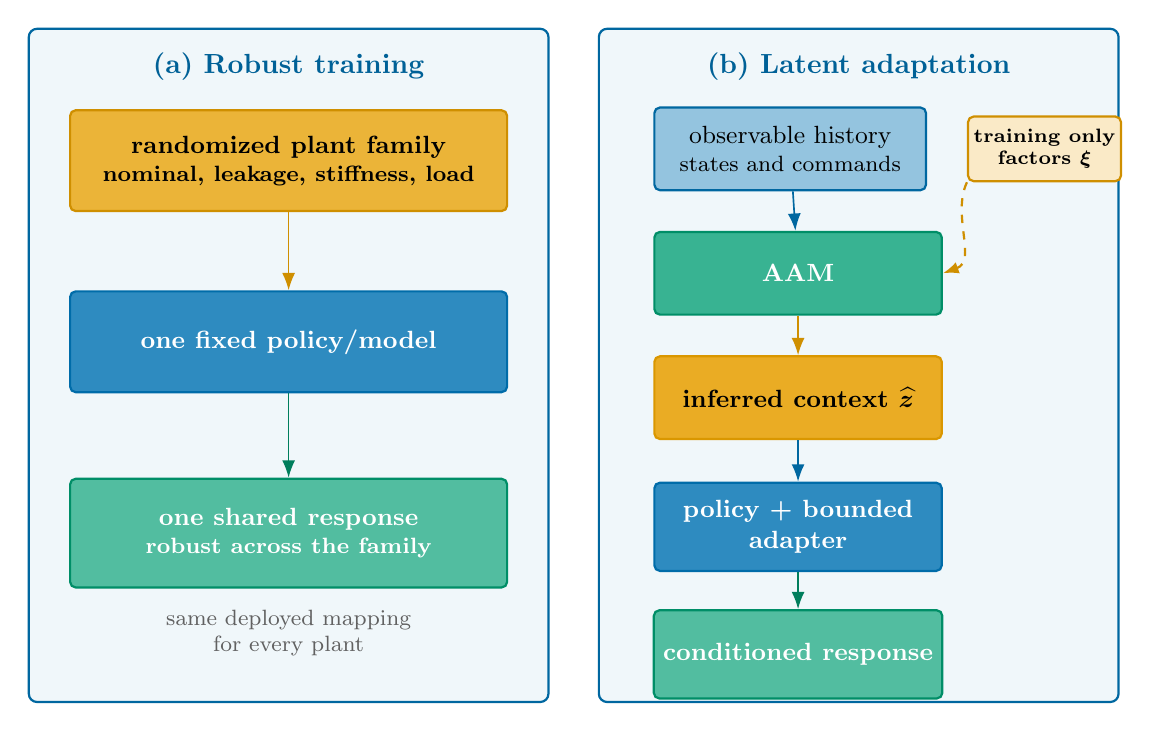
\begin{tikzpicture}[x=1cm,y=1cm,>=Latex,font=\small]
  % Reuse the node colors, line weights and rounded geometry of Figure 3.7.
  \node[draw=cbblue!90!black,line width=.8pt,rounded corners=3pt,
    fill=cbblue!6,minimum width=6.60cm,minimum height=8.55cm] (robustpanel) at (-3.62,-4.05) {};
  \node[font=\normalsize\bfseries,text=cbblue!85!black] at (-3.62,-.25)
    {(a) Robust training};

  \node[draw=cborange!90!black,line width=.8pt,rounded corners=2pt,
    fill=cborange!78,minimum width=5.55cm,minimum height=1.28cm,
    align=center,font=\small\bfseries] (familyR) at (-3.62,-1.45)
    {randomized plant family\\[-1pt]\footnotesize nominal, leakage, stiffness, load};
  \node[draw=cbblue!95!black,line width=.8pt,rounded corners=2pt,
    fill=cbblue!82,text=white,minimum width=5.55cm,minimum height=1.28cm,
    align=center,font=\small\bfseries] (fixed) at (-3.62,-3.75)
    {one fixed policy/model};
  \node[draw=cbgreen!90!black,line width=.8pt,rounded corners=2pt,
    fill=cbgreen!68,text=white,minimum width=5.55cm,minimum height=1.38cm,
    align=center,font=\small\bfseries] (shared) at (-3.62,-6.18)
    {one shared response\\[-1pt]\footnotesize robust across the family};
  \draw[sigarrow,cborange!90!black] (familyR) -- (fixed);
  \draw[sigarrow,cbgreen!80!black] (fixed) -- (shared);
  \node[font=\footnotesize,text=black!62,align=center] at (-3.62,-7.45)
    {same deployed mapping\\for every plant};

  \node[draw=cbblue!90!black,line width=.8pt,rounded corners=3pt,
    fill=cbblue!6,minimum width=6.60cm,minimum height=8.55cm] (adaptpanel) at (3.62,-4.05) {};
  \node[font=\normalsize\bfseries,text=cbblue!85!black] at (3.62,-.25)
    {(b) Latent adaptation};

  \node[draw=cbblue!90!black,line width=.8pt,rounded corners=2pt,
    fill=cbblue!42,minimum width=3.45cm,minimum height=1.05cm,
    align=center,font=\small] (history) at (2.75,-1.30)
    {observable history\\[-1pt]\footnotesize states and commands};
  \node[draw=cbgreen!90!black,line width=.8pt,rounded corners=2pt,
    fill=cbgreen!78,text=white,minimum width=3.65cm,minimum height=1.05cm,
    align=center,font=\small\bfseries] (aam) at (2.85,-2.88)
    {AAM};
  \node[draw=cborange!95!black,line width=.8pt,rounded corners=2pt,
    fill=cborange!86,minimum width=3.65cm,minimum height=1.05cm,
    align=center,font=\small\bfseries] (latent) at (2.85,-4.46)
    {inferred context $\widehat{\bm{z}}$};
  \node[draw=cbblue!95!black,line width=.8pt,rounded corners=2pt,
    fill=cbblue!82,text=white,minimum width=3.65cm,minimum height=1.12cm,
    align=center,font=\small\bfseries] (mapping) at (2.85,-6.10)
    {policy + bounded\\adapter};
  \node[draw=cbgreen!90!black,line width=.8pt,rounded corners=2pt,
    fill=cbgreen!68,text=white,minimum width=3.65cm,minimum height=1.12cm,
    align=center,font=\small\bfseries] (response) at (2.85,-7.72)
    {conditioned response};

  \draw[sigarrow,cbblue!90!black] (history) -- (aam);
  \draw[sigarrow,cborange!90!black] (aam) -- (latent);
  \draw[sigarrow,cbblue!90!black] (latent) -- (mapping);
  \draw[sigarrow,cbgreen!80!black] (mapping) -- (response);

  \node[draw=cborange!90!black,line width=.8pt,rounded corners=2pt,
    fill=cborange!22,minimum width=1.45cm,minimum height=.82cm,
    align=center,font=\scriptsize\bfseries,inner sep=2pt] (teacher) at (5.98,-1.30)
    {training only\\factors $\bm{\xi}$};
  \draw[-{Latex[length=2.0mm]},line width=.8pt,dashed,cborange!90!black]
    (teacher.south west) to[out=-115,in=20] (aam.east);
\end{tikzpicture}

  \caption{Canonical latent-adaptation architecture contrasted with robust
  training. The architecture motivates the offline identifiability study; the
  final AF implementation instead learns its context representation end to end
  from the control objective.}
  \label{fig:fund:robust-adaptive}
\end{figure}

Teacher--student methods encode known simulation factors into a privileged
latent and train an estimator to recover it from observable history. The
construction generalises the wider privileged-learning idea, in which a teacher
with access to unavailable state supervises a student restricted to deployable
observations~\cite{chen2019cheating}. Lee et al.~\cite{lee2020learning} used it
for hidden terrain properties; Kumar et al.~\cite{kumar2021rma} developed rapid
motor adaptation; Miki et al.~\cite{miki2022perceptive} extended the same
teacher--student route to fusing proprioception with exteroception under
unreliable perception. Distillation from a privileged teacher is the mechanism
this thesis uses in Chapter~\ref{chap:control}, with a classical controller in
the teacher's place rather than a privileged
policy~\cite{ross2011reduction}. All of them assume that the factor directions
the estimator retains are the directions the controller needs. Liu et al.~\cite{liu2025frma} report the failure when it
does not hold, where a low-dimensional adapter drops factors that act through
separate channels, and add training phases to recover them. Chapter~\ref{chap:models} finds the same
mismatch here in a sharper form, and the finding is quoted forward because it
is why the deployed stack departs from this line: what an unconstrained
estimate carries here is mainly seal condition, which acts through pressure, and
pressure is the one channel the controller does not integrate
(Section~\ref{sec:models:aam-content}). The deployed controller therefore
conditions on a single physical quantity it can act on, the payload, rather than
on a learned code.

Unlike classical online parameter estimation~\cite{astrom1995adaptive}, the
learned latent need not have a direct physical interpretation. It can be given
one. Hu et al.~\cite{hu2026bayesian} estimate named physical quantities on an
excavator arm with Bayesian reinforcement learning, which buys interpretation
at the price of the explicit plant model that
Section~\ref{sec:fund:conventional-control} identified as the maintenance
burden. The latent used here is anonymous and is therefore audited for content
rather than read as parameters. A latent can also condition a dynamics model
instead of a policy, as in the contextual neural ODE of Yu et
al.~\cite{yu2026context}. That is the nearest relative of the route taken here,
with one difference that decides the outcome: in \ppoAAMFD{} the conditioning
enters the command path rather than the predictor, because a better prediction
helps only if something downstream acts on it.

The offline AAM developed in Chapter~\ref{chap:models} tests whether one second
of observable history contains recoverable plant information. It is not the
encoder deployed in AF, which trains its own history encoder end to end with
the residual under the task objective rather than against an offline target
(Section~\ref{sec:ctrl:af-encoder} details the training scheme). The two routes
therefore answer different questions: the former tests identifiability; the
latter tests control-relevant adaptation. The experiments also keep robust
randomised training distinct from both routes.

Randomised training produces a single controller for a family of plants.
Identification of that family is what makes a member-specific correction
possible. In canonical latent adaptation, adaptation is the online use of that
identification: the controller infers which plant is present from observable
history and conditions the command on that estimate. The two responses are
therefore sequential, not alternatives.

\section{Reinforcement Learning and Structured Priors}
\label{sec:fund:rl-residual}

\subsection{Policy Optimisation}

Reinforcement learning optimises a policy from observations to actions for
expected cumulative reward~\cite{sutton2018reinforcement}. This thesis uses
PPO~\cite{schulman2017proximal} with generalised advantage estimation
~\cite{schulman2016gae}; Section~\ref{sec:ctrl:optimization} gives the exact
objective. GPU-parallel simulation supplies the required throughput
~\cite{makoviychuk2021isaac,rudin2022learning}, which is why compact actuator
surrogates replace the full hydraulic plant during training.

\subsection{Structured Priors for Policy Learning}
\label{sec:fund:prior}

Learning from scratch would discard reliable kinematics. Residual RL instead
adds a bounded learned correction to a controller at runtime
~\cite{johannink2019residual,silver2018residual}. Policy distillation moves the
prior to training: a privileged DLS teacher supplies demonstrations, then the
student acts alone~\cite{ross2011reduction}. This thesis takes the second
route. The teacher is distilled and PPO updates are anchored to the frozen
student (Section~\ref{sec:ctrl:anchored}), and the deployed actor remains the
sole controller: no analytic controller runs underneath it at deployment, so
the runtime correction of residual RL is not the construction used here.

One clarification belongs here, because the vocabulary collides. The adaptive
stack of Chapter~\ref{chap:control} does modify its own frozen actor, but not by
adding a residual in the sense of this subsection. There is no classical
controller beneath it to correct, and its purpose is not to supply a prior that
accelerates learning. It is an online adaptation mechanism internal to the
reinforcement-learning policy, whose only function is to carry the dependence on
inferred plant context that a frozen actor cannot express. It therefore belongs
to the adaptation line of
Section~\ref{sec:fund:adaptation} and is compared against that literature, not
against residual policy learning.

The idea parallels real-world fine-tuning that retains a simulation-trained
value function~\cite{yin2025rapidly}, but here the retained object is the
reference policy. Anchoring was introduced because unconstrained PPO improved
reward while degrading the physical tracking criterion
(Section~\ref{sec:ctrl:training}).

\subsection{Reinforcement Learning on Hydraulic Machines}

Deep RL has reached full-size hydraulic machines. What distinguishes those
stacks from the one built here is not scale but the level at which the policy
commands the machine, because that level decides how much of the hydraulic
chain of Section~\ref{sec:fund:actuation-chain} the policy has to represent at
all.

Egli and Hutter~\cite{egli2020towards} trained an excavator-arm policy in
simulation and transferred it to a full-size walking excavator, then generalised
the construction across excavation tasks~\cite{egli2022general}. The policy
acts on joint-level velocity references, and a low-level tracking layer on the
machine converts them into valve currents. Spinelli et
al.~\cite{spinelli2024rl} keep that division on a commercial material handler
and add an underactuated tool, so the policy has to exploit passive tool
dynamics rather than command them, while the actuated joints are still driven
through the same kind of tracking layer. In both cases the orifice
nonlinearity, the dead zone, the directional asymmetry and the load dependence
live below the learned policy, in a layer that was identified and calibrated for
that machine before the policy existed.

That division is sound where the tracking layer already exists. It is not
available here for two reasons. The FME~500 is a series road-maintenance
implement with no calibrated joint-velocity layer to inherit, and building one
is precisely the per-machine identification that
Section~\ref{sec:fund:conventional-control} identified as the maintenance cost
of the model-based families. More importantly, a velocity interface hides the
quantity this thesis sets out to measure. If the layer beneath the policy
already owns the command-to-motion mapping, the question of whether a learned
actuator retains command authority under saturation and dead zone cannot be
posed at all; it has been answered by construction, once, by hand. The stacks
here therefore command the actuator directly, either as a cylinder increment
realised by a learned model or, in \ppoAAMFD, as the valve command itself.

Maitan et al.~\cite{maitan2026contraction} take the opposite position and train
on the physical cylinder, bounding exploration with a contraction-metric
filter. That work does command the actuator at the low level, and training on
hardware removes the transfer question outright. The result is force control on
a single actuator on a test bench, and it does not obviously scale to a
multi-link boom on a moving carrier, where the exploration the policy needs is
the exploration the filter has to prevent.

These studies settle scale and feasibility. In each of them the actuator
representation is a fixed design choice inside the stack rather than a
variable, so none separates the transfer result from the representation that
produced it. That separation is criterion V below.

None of these stacks varies the plant within a deployment. They are trained for
robustness across one machine and its payload or soil conditions, and a plant
that changes during a run is outside the construction. What remains open is the
combination: a randomised plant family, online actuator adaptation, a
privileged kinematic teacher, and a matched comparison of actuator
representations under one protocol.

A policy can also compensate for a poor actuator model. Chapter
~\ref{chap:evaluation} therefore reports rollout error, command magnitude and
smoothness, and cylinder-level residuals alongside task tracking. Equal task
error alone is not evidence of equal model quality.

\section{Research Gap and Thesis Positioning}
\label{sec:fund:gap}

The literature leaves a specific combination unresolved. Hydraulic control
provides structure but requires maintained plant models; learned dynamics
replace derivation with data but depend on identifiable excitation; actuator
surrogates and latent adaptation are established mainly for electric legged
robots; and hydraulic RL studies do not isolate actuator representation under
a matched protocol. Table~\ref{tab:fund:positioning} summarises this position.

The five criteria are: (I) learned hydraulic actuation, (II) data audited for
causal input identifiability, (III) online adaptation to plant variation at
deployment, (IV) a classical-control prior transferred through policy
distillation, and (V) a matched actuator comparison.

What the table does and does not assert is worth fixing before it is read. The
rows are lines of work, not individual papers, and the criteria are the ones
this thesis needs rather than a neutral taxonomy of the field. Every criterion
is individually established somewhere, several of them for decades, and
single works cover more of a row than a coarse mark can show. The latent
adaptation row in particular samples a large and active literature; it is read
here for the assumption those constructions share, that the factor directions
an estimator retains are the directions the controller needs, and not for
coverage. The claim is the combination on one machine under one protocol, and
Column III shows how narrow even that claim becomes once it is measured rather
than designed for.

\begin{table}[H]
  \centering
  \caption{Positioning against the reviewed lines of work. Parenthesized marks
  denote partial or implicit coverage. Column III is parenthesized for this
  thesis because the deployed route conditions on a single estimated physical
  quantity rather than on the learned latent of
  \cite{lee2020learning,kumar2021rma}, and because its benefit is confined to
  the loaded regime (Section~\ref{sec:eval:adaptation}).}
  \label{tab:fund:positioning}
  \small
  \setlength{\tabcolsep}{3pt}
  \begin{tabular}{@{}p{.69\textwidth}ccccc@{}}
    \toprule
    Line of work & I & II & III & IV & V \\
    \midrule
    \raggedright Model-based hydraulic control\\[-1pt]
      {\scriptsize\cite{mattila2017survey,jelali2003hydraulic}}
      & --- & ($\checkmark$) & ($\checkmark$) & $\checkmark$ & --- \\
    \raggedright Actuator networks for legged robots\\[-1pt]
      {\scriptsize\cite{hwangbo2019learning,rudin2022learning,yamamori2026actuator}}
      & --- & $\checkmark$ & --- & --- & --- \\
    \raggedright RL for hydraulic machines\\[-1pt]
      {\scriptsize\cite{egli2020towards,egli2022general,spinelli2024rl,maitan2026contraction}}
      & $\checkmark$ & ($\checkmark$) & --- & --- & --- \\
    \raggedright Latent online adaptation\\[-1pt]
      {\scriptsize\cite{lee2020learning,kumar2021rma,yu2026context,liu2025frma,hu2026bayesian}}
      & --- & --- & $\checkmark$ & --- & --- \\
    \raggedright Residual RL and policy distillation\\[-1pt]
      {\scriptsize\cite{johannink2019residual,silver2018residual,ross2011reduction,yin2025rapidly}}
      & --- & --- & --- & $\checkmark$ & --- \\
    \midrule
    This thesis (\ppoROM{} / \ppoIDFD{} / \ppoAAMFD)
      & $\checkmark$ & $\checkmark$ & ($\checkmark$) & $\checkmark$ & $\checkmark$ \\
    \bottomrule
  \end{tabular}
\end{table}

Column III carries a parenthesis, and the reason is specific. What
\ppoAAMFD{} deploys is a policy conditioned on one estimated physical quantity,
the payload, recovered online from the task observation it already carries,
rather than the anonymous latent of the canonical architecture.
Section~\ref{sec:eval:adaptation} measures what that conditioning recovers, in
which payload regime it helps, and how much of the gain survives when the
payload is permuted across environments.

The contribution remains the complete experimental chain: identifiable cylinder
data, structurally constrained models fast enough for parallel training, online
adaptation and a common evaluation protocol. Adaptation is reported as a
conditional mechanism, with positive and negative training seeds kept in the
same analysis. The three tested stacks are:

\begin{description}
  \item[\ppoROM.] A command-conditioned ROM realises the policy's desired
    cylinder motion. It is the reference and the only actuator calibrated to
    the deployment plant (Section~\ref{sec:ctrl:constraints}).
  \item[\ppoIDFD.] The same policy interface drives the frozen inverse model
    followed by the strict forward model, forming the robust learned
    baseline.
  \item[\ppoAAMFD.] The policy emits the valve command directly and the
    inverse model leaves the path. A causal history encoder conditions a
    bounded residual on that command, which the same forward model realises
    ahead of PhysX.
\end{description}

All stacks share the task, terrain, trajectories, deployment factors and
evaluation gates. \ppoROM{} and \ppoIDFD{} additionally share the action
contract and form the matched pair; \ppoAAMFD{} does not, because its policy
chooses a valve command rather than a cylinder increment, and it is therefore
compared with its own frozen base rather than ranked against the others. The
ROM is calibrated to the deployment plant, so causal architectural claims rely
on the matched pair and on within-stack paired ablations rather than on a
three-way contrast (Section~\ref{sec:ctrl:matching}). Chapter~\ref{chap:system}
now grounds this comparison in the concrete machine.

The remaining gap concerns the interaction between these established
techniques: whether hydraulic actuators identified for control retain command
authority after transfer, and under which plant conditions a
history-conditioned correction on the identified valve path adds value beyond
randomisation and matched residual capacity.

\RRLABchapterblank
%%%%%%%%%%%%%%%%%%%%%%%%%%%%%%%%%%%%%%%%%%%%%%%%%%%%%%%%%%%%
%% Chapter 3 — System Fundamentals and Problem Formulation
%% (10–15 pages)
%% Purpose: describe the physical and simulated system once,
%% define all coordinate spaces and interfaces, and formulate
%% the control objective mathematically.
%%%%%%%%%%%%%%%%%%%%%%%%%%%%%%%%%%%%%%%%%%%%%%%%%%%%%%%%%%%%
\chapter{System Fundamentals and Problem Formulation}
\label{chap:system}

Chapter~\ref{chap:fundamentals} established the control and modeling concepts
used in this thesis. This chapter converts that background into a fixed system
definition for the remaining work. It specifies the physical mechanism,
coordinate mappings, available measurements, actuator models, task geometry,
and evaluation interfaces before the controllers are compared. Keeping these
definitions together prevents later chapters from changing the plant,
observation set, or success criteria when interpreting results.

The physical machine and its two simulation representations are distinguished
explicitly. Simscape is the high-fidelity hydraulic source used for actuator
identification. IsaacLab/PhysX is the parallel environment used for policy
training, adaptation-data collection, and closed-loop evaluation. Both use the
cylinder ordering, kinematics, action contract, and cutter-tip task variables
defined here, but they are not assumed to be identical plants.

Sections~\ref{sec:sys:platform}--\ref{sec:sys:actuation} define the mechanism,
coordinate spaces, and signals. Sections~\ref{sec:sys:simscape} and
\ref{sec:sys:isaaclab} describe the two simulation models. The remaining
sections define the verge-following task, the R, IF, and AIF control stacks,
the control objective, and the acceptance gates used in the experiments.

\section{Manipulator Platform}
\label{sec:sys:platform}

The MULAG FME~500 is modeled as a serial-link mechanism with five
revolute joints. Four hydraulic
cylinders actuate the slew, two boom, and head-pivot joints. The
\emph{Messerkopf} rotation has no independent actuator and is locked at
the mowing configuration; it is therefore not a controlled degree of
freedom. The cylinder order used throughout the thesis is slew
(\emph{Drehzapfen}), boom~I (\emph{Ausleger~I}), boom~II
(\emph{Ausleger~II}), and head pivot (\emph{Messerkopf-Schwenk}).

Table~\ref{tab:sys:cylinders} gives the cylinder stroke ranges used in
the training data and the fixed limit of the \emph{Messerkopf} joint.
Task-space errors are measured at the cutter tip, which lies
$\unit[0.79]{m}$ below the \emph{Messerkopf} body origin.

\begin{table}[htbp]
  \centering
  \caption{Cylinder stroke ranges in the training data
  (Chapter~\ref{chap:data}) and the fixed \emph{Messerkopf} joint limit
  used for the mowing task.}
  \label{tab:sys:cylinders}
  \begin{tabular}{clcc}
    \toprule
    $i$ & Joint & Function & Limit \\
    \midrule
    1 & \emph{Drehzapfen}         & slew       & $0.018$--$0.493\,\mathrm{m}$ \\
    2 & \emph{Ausleger I}         & boom I     & $0.275$--$0.791\,\mathrm{m}$ \\
    3 & \emph{Ausleger II}        & boom II    & $0.309$--$0.857\,\mathrm{m}$ \\
    4 & \emph{Messerkopf-Schwenk} & head pivot & $0.269$--$0.689\,\mathrm{m}$ \\
    \midrule
    5 & \emph{Messerkopf}         & head rotation (locked) & $q_{5,\min}=q_{5,\max}=q_{5,\mathrm{lock}}$ \\
    \bottomrule
  \end{tabular}
\end{table}

Figure~\ref{fig:sys:topology} identifies the links, joints, and four actuator
channels used throughout the model.

\begin{figure}[htbp]
  \centering
  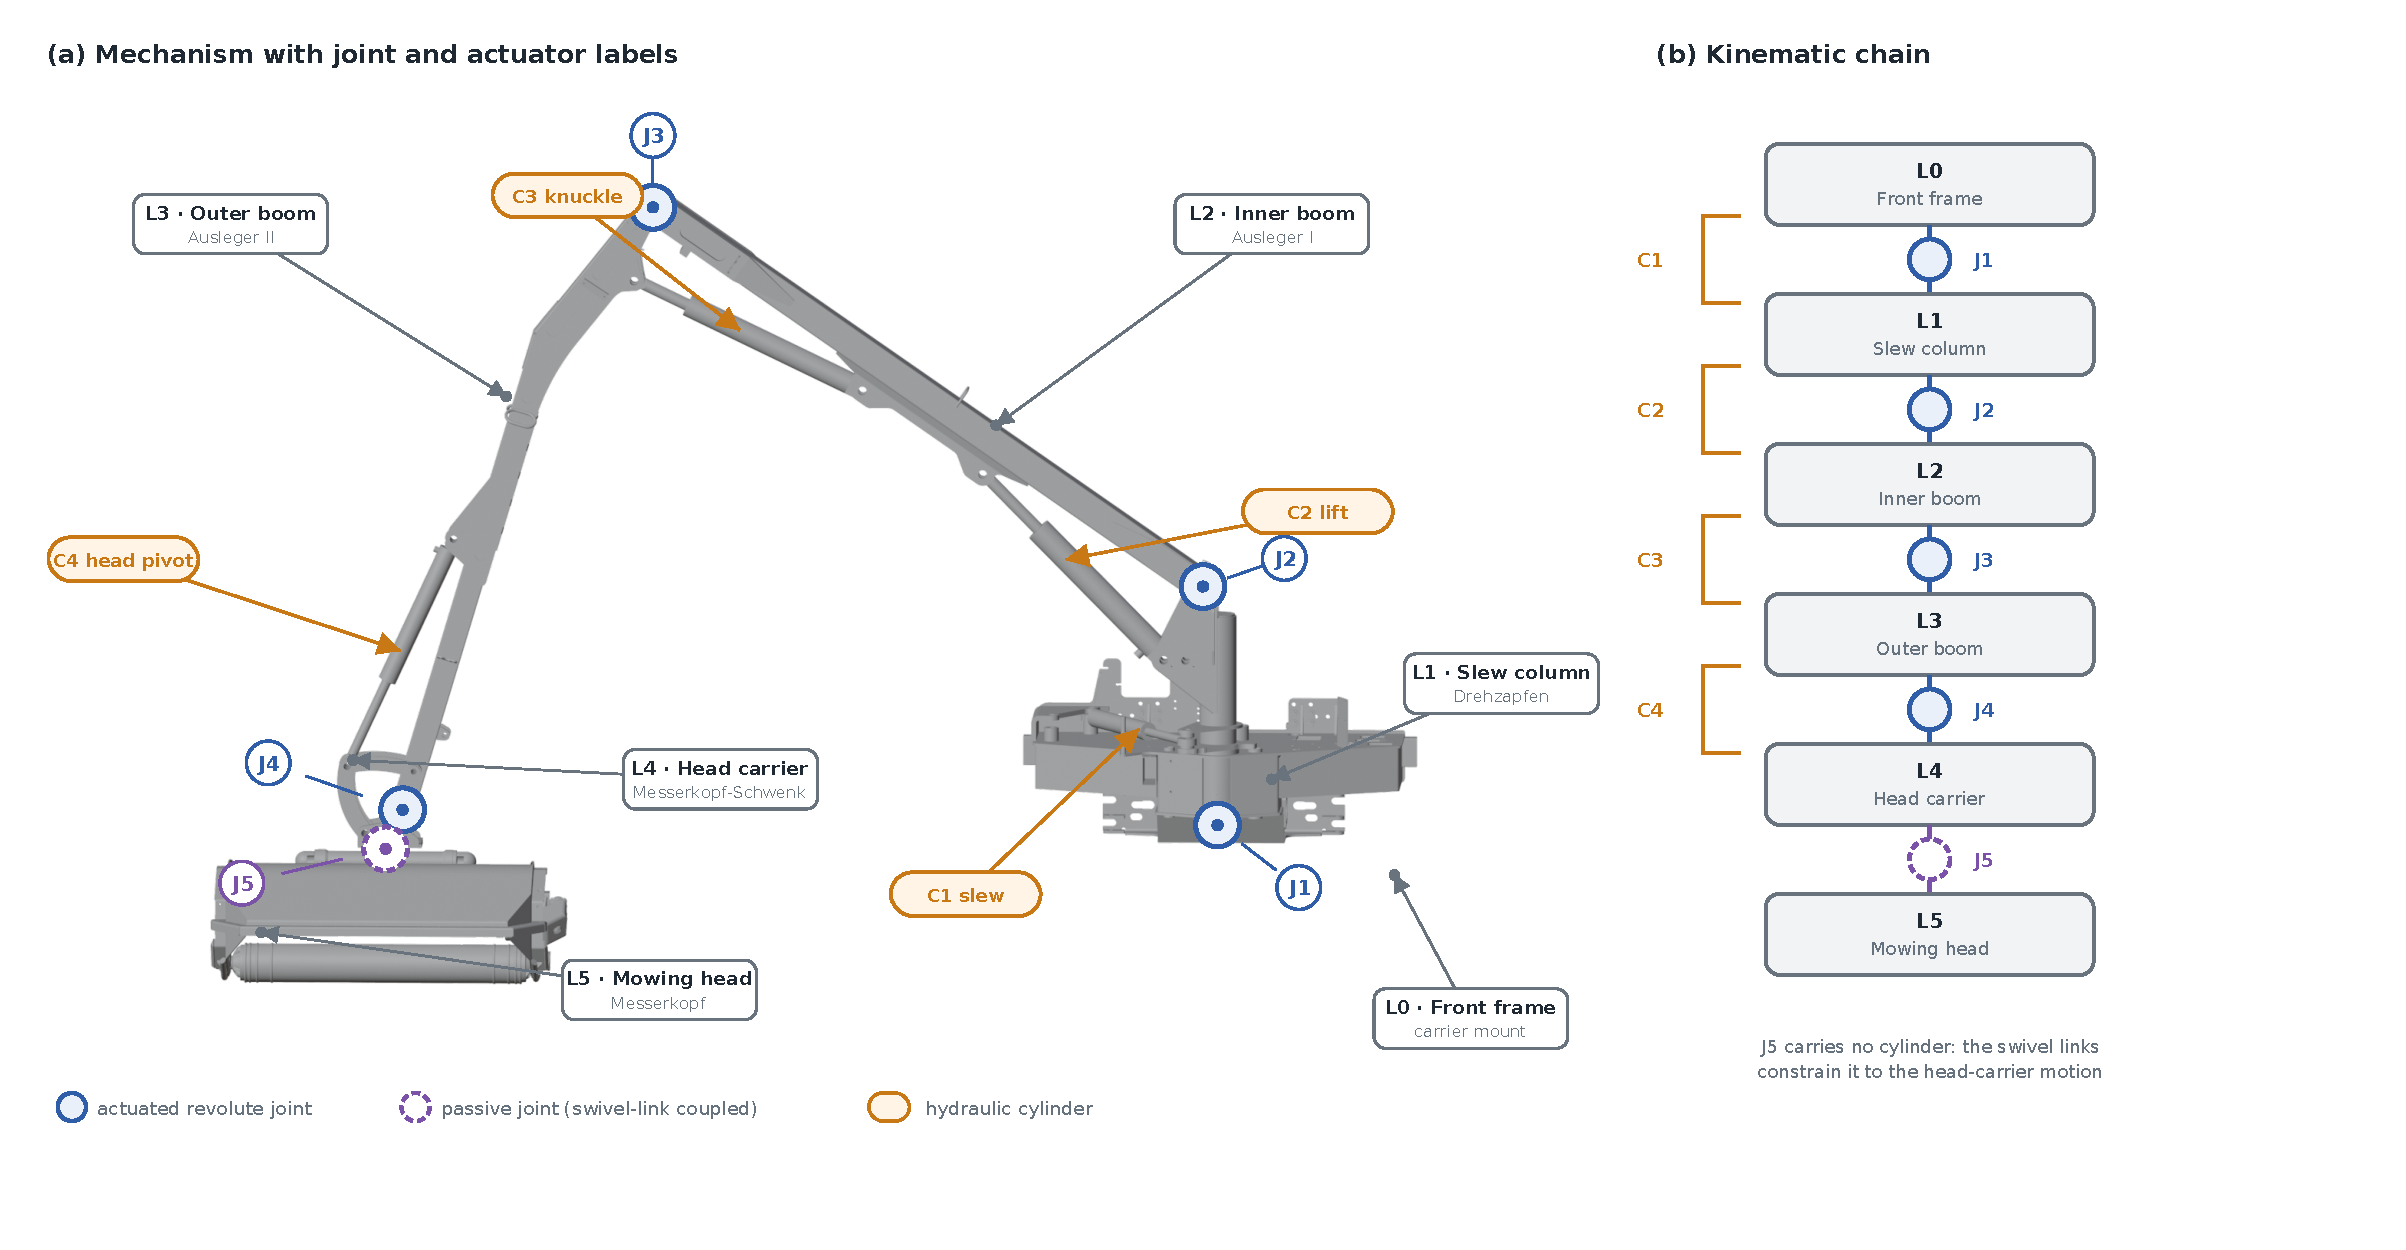
\includegraphics[width=\textwidth,trim=0 0 375 0,clip]{images/fme500_topology_annotated}
  \caption{Annotated CAD view of the MULAG FME~500. Links L0--L5,
  joints J1--J5, and the four hydraulic cylinders C1--C4 are identified;
  J5 denotes the \emph{Messerkopf} rotation, which is locked in the
  mowing configuration used in this thesis.}
  \label{fig:sys:topology}
\end{figure}

Figure~\ref{fig:sys:link-catalog} separates the rigid bodies that form the
assembled mechanism. The catalog makes the L0--L5 body assignment explicit
and shows the representative barrel--rod geometry used for cylinders C1--C4.

\begin{figure}[htbp]
  \centering
  \newcommand{\partcell}[4]{%
    \begin{minipage}[t]{.225\textwidth}
      \centering
      \textbf{\textcolor{#4}{#1}}\par
      \includegraphics[width=.96\linewidth]{images/links/#2}\par
      \vspace{-1mm}\small #3
    \end{minipage}}
  \partcell{L0}{link_frontrahmen}{Front frame}{cbblue}\hfill
  \partcell{L1}{link_drehzapfen}{Slew column}{cbblue}\hfill
  \partcell{L2}{link_ausleger_i}{Inner boom}{cbblue}\hfill
  \partcell{L3}{link_ausleger_ii}{Outer boom}{cbblue}

  \vspace{3mm}
  \makebox[\textwidth][c]{%
    \partcell{L4}{link_messerkopf_schwenk}{Head carrier}{cbblue}\hspace{.025\textwidth}%
    \partcell{L5}{link_messerkopf}{Mowing head}{cbblue}\hspace{.025\textwidth}%
    \partcell{C1--C4}{link_cylinder}{Double-acting cylinder}{cborange}}
  \caption{Individual CAD-derived bodies of the MULAG FME~500 shown at a
  common orthographic scale. L0--L5 are the front frame, slew column, inner
  boom, outer boom, head carrier, and mowing head. The C1--C4 panel shows the
  representative double-acting cylinder barrel--rod pair.}
  \label{fig:sys:link-catalog}
\end{figure}

Manufacturer CAD supplies the link geometry, joint locations, masses, centers
of mass, and inertia tensors through Phobos~\cite{vonszadkowski2020phobos}.
The same CAD-derived bodies and joint frames form the mechanical basis of the
Simscape and IsaacLab models, keeping dimensions, axes, masses, and cylinder
lever arms consistent while the hydraulic implementations remain
model-specific.

\section{Kinematic Structure and Coordinate Mappings}
\label{sec:sys:kinematics}

\subsection{Joint Space and Cylinder Space}

The configuration is $\bm{q} \in \mathbb{R}^5$; the actuated coordinates are
the four cylinder extensions $\bm{x} \in \mathbb{R}^4$. Cylinder $i$ joins CAD
attachment points $\bm{p}_A$ and $\bm{p}_B$ on adjacent links. Its length and
extension are
%
\begin{equation}
  \label{eq:sys:cyl-length}
  \ell_i(\bm{q}) = \bigl\| \bm{p}_B(\bm{q}) - \bm{p}_A(\bm{q}) \bigr\|,
  \qquad
  x_i = \ell_i(\bm{q}) - \ell_{0,i},
\end{equation}
%
with $\ell_{0,i}$ the retracted reference length. Differentiating
\eqref{eq:sys:cyl-length} gives the scalar mapping between joint motion
and extension rate,
%
\begin{equation}
  \label{eq:sys:cyl-jac}
  \dot{x}_i = J_{\mathrm{cyl},i}(\bm{q})\, \dot{\bm{q}},
  \qquad
  J_{\mathrm{cyl},i} = \bm{e}_i^{\!\top}
  \bigl( \bm{J}_B - \bm{J}_A \bigr),
\end{equation}
%
where $\bm{e}_i$ is the cylinder-axis unit vector and $\bm{J}_A$ and
$\bm{J}_B$ are attachment-point Jacobians. Virtual work gives
$\bm{\tau}_{\mathrm{act}}=\bm{J}_{\mathrm{cyl}}^{\top}\bm{F}_h$.
The mapping varies with configuration and stroke.

\subsection{Task Space and the Calibrated Cutter Jacobian}
\label{sec:sys:task-jacobian}

The cutter tip is expressed in the truck chassis frame
(\texttt{base\_link}); using the moving slew-base frame would corrupt the
tracking error. The controlled point includes the $\unit[-0.79]{m}$ tool-tip
offset. Vehicle motion supplies the along-track direction.

The calibrated Jacobian $\bm{J}_c\in\mathbb{R}^{3\times4}$ maps cylinder
extension rates to cutter-tip velocity. It was measured at the head-down
mowing pose by stepping each cylinder target and recording the settled cutter
displacement. Its singular values are $8.24$, $5.69$, and $2.79$, giving
rank~3. The damped least-squares controller in Chapter~\ref{chap:control}
uses this same Jacobian.

\section{Actuation and Measured State}
\label{sec:sys:actuation}

Table~\ref{tab:sys:signals} lists the signals and their availability.

\begin{table}[htbp]
  \centering
  \caption{Signal inventory of the modeled system. ``S'' marks signals
  present in the Simscape data exports, ``I'' signals available live in
  the IsaacLab environment, ``M'' quantities that exist there only
  through the learned models of Chapter~\ref{chap:models}, and ``P''
  \emph{privileged} quantities that exist in simulation but must never
  enter a deployable policy or estimator input.}
  \label{tab:sys:signals}
  \small
  \begin{tabular}{@{}llcl@{}}
    \toprule
    Signal & Dimension & Availability & Meaning \\
    \midrule
    $\bm{u}$ & $[-1,1]^4$ & S, M & normalized proportional-valve commands \\
    $\bm{x},\, \dot{\bm{x}}$ & $\mathbb{R}^4$ & S, I & cylinder extensions and velocities \\
    $\Delta\bm{p}$ & $\mathbb{R}^4$ & S, M & chamber pressure differences \\
    $\bm{F}$ & $\mathbb{R}^4$ & S & logged rod forces \\
    $\bm{q},\, \dot{\bm{q}}$ & $\mathbb{R}^5$ & S, I & joint positions and velocities \\
    $\bm{p}_c$ & $\mathbb{R}^3$ & S, I & cutter-tip position, truck frame \\
    $\bm{h}$ & $\mathbb{R}^{9}$ & I & forward terrain-height profile ahead of the cutter \\
    $\bm{c} = [\Delta\bm{x}^*, \Delta\dot{\bm{x}}^*]$ & $\mathbb{R}^8$ & I & desired cylinder command \\
    $\factorvec$ & $\mathbb{R}^6$ & P & physical randomization factors of the active plant \\
    $\bm{z} = \mu(\factorvec)$ & $\mathbb{R}^{d_z}$ & P & privileged dynamics latent, $d_z = 2$ \\
    $\latenthat$ & $\mathbb{R}^{d_z}$ & M & AAM estimate of $\bm{z}$ from observable history \\
    \bottomrule
  \end{tabular}
\end{table}

In IsaacLab, valve commands and differential pressures are learned-actuator
states, not direct measurements. R produces them internally; IF and AIF obtain
them from the inverse/forward pair. $\factorvec$ and
$\bm{z}=\mu(\factorvec)$ are privileged; only $\latenthat$ may enter AIF.

\subsection{Sensing and Observability}
\label{sec:sys:sensing}

The deployable observation contains articulation state, terrain rays, contact
signals, the desired cylinder command, and actuator-model pressure state. Plant
parameters are not observed; AIF infers their effect from causal history.

\begin{figure}[htbp]
  \centering
  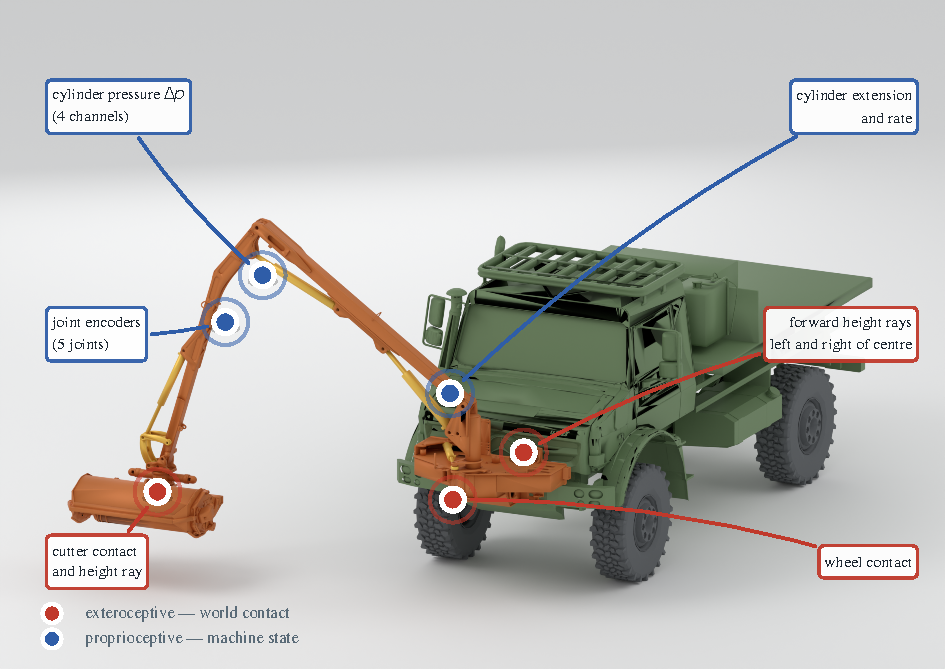
\includegraphics[width=.92\textwidth]{images/ch3_sensor_map}
  \caption{Sensor and observability map for the deployed
  controller. Blue callouts identify proprioceptive inputs: joint encoders,
  cylinder pressure differences, and cylinder extension and rate. Red
  callouts identify exteroceptive inputs: forward terrain-height rays and
  cutter and wheel contact.}
  \label{fig:sys:sensing}
\end{figure}

Figure~\ref{fig:sys:sensing} separates deployable measurements from
privileged plant information. Articulation state is read from the physics
engine without encoder noise or
quantisation.

\section{High-Fidelity Simscape Model}
\label{sec:sys:simscape}

The actuator models use a multi-domain Simscape model of the FME~500 developed
in the preceding master project. Table~\ref{tab:sys:provenance} distinguishes
the data source of each frozen component.

\begin{table}[htbp]
  \centering
  \caption{Provenance of each frozen actuator component. The command ROM
  is the only one that has been calibrated against the deployment plant;
  the inverse/forward pair is Simscape-identified throughout. This
  asymmetry is a property of the comparison and is carried into the
  discussion of Chapter~\ref{chap:evaluation}, not glossed over.}
  \label{tab:sys:provenance}
  \small
  \begin{tabular}{lp{4.4cm}p{5.0cm}}
    \toprule
    Component & Identified on & Calibrated on \\
    \midrule
    Command ROM & Simscape closed-loop export (grey-box, full model)
      & IsaacLab/PhysX closed-loop rollouts, via a bounded command-gated
        correction head only \\
    Control ID & Simscape closed-loop export & --- \\
    Strict FD & Simscape closed-loop export, retrained on the strict
        open-loop excitation export & --- \\
    $SD_0$, $\mu(\factorvec)$, $SD_z$, AAM
      & IsaacLab/PhysX adaptation collection (from scratch) & --- \\
    \bottomrule
  \end{tabular}
\end{table}

Simscape supplies the frozen ID and strict FD checkpoints. The ROM receives an
additional bounded IsaacLab calibration
(Section~\ref{sec:models:rom-calibration}). The adaptation models are trained
from IsaacLab data collected through the ROM and PhysX.

\subsection{The Command ROM as Deployment Actuator}
\label{sec:sys:rom-is-plant}

The command ROM plus PhysX is the deployment plant. Simscape is too slow for
policy training and bare PhysX has no hydraulics. The ROM is therefore both the
plant model and the actuator of R:

\begin{itemize}
  \item R uses the deployment plant itself and is the reference condition.
  \item IF replaces it with an independently identified inverse/forward pair.
  \item AIF adds online adaptation to IF.
\end{itemize}

The R--IF gap measures the transfer cost of the independently identified pair;
it is not a general ranking of the two model classes.

\subsection{Mechanical Subsystem}

The mechanism uses the CAD-derived links, joints, and cylinder attachment
frames of Section~\ref{sec:sys:platform}. It is simulated in Simscape
Multibody \cite{mathworks2024simscapemultibody}. The joint-space dynamics take
the standard manipulator form
%
\begin{equation}
  \label{eq:sys:eom}
  \bm{M}(\bm{q})\ddot{\bm{q}}
  + \bm{C}(\bm{q},\dot{\bm{q}})\dot{\bm{q}}
  + \bm{g}(\bm{q})
  + \bm{\tau}_{\mathrm{fric}}(\dot{\bm{q}})
  = \bm{\tau}_{\mathrm{act}} - \bm{J}^{\top}(\bm{q})\,\bm{F}_{\mathrm{ext}},
\end{equation}
%
with inertia $\bm{M}$ from the imported CAD. Friction combines viscous,
Coulomb, and Stribeck terms. The cutting load scales with feed velocity and
vegetation density. Each cylinder uses a
spherical--prismatic--cylindrical loop and hard stops enforce the limits in
Table~\ref{tab:sys:cylinders}.

\subsection{Hydraulic Subsystem}

Figure~\ref{fig:sys:schematic} shows four 4/3 valve-driven asymmetric cylinders
fed by a variable-speed, fixed-displacement pump
($Q_p=D_p\omega$), accumulator, and pressure-relief valve.

\begin{figure}[htbp]
  \centering
  \resizebox{\textwidth}{!}{%
  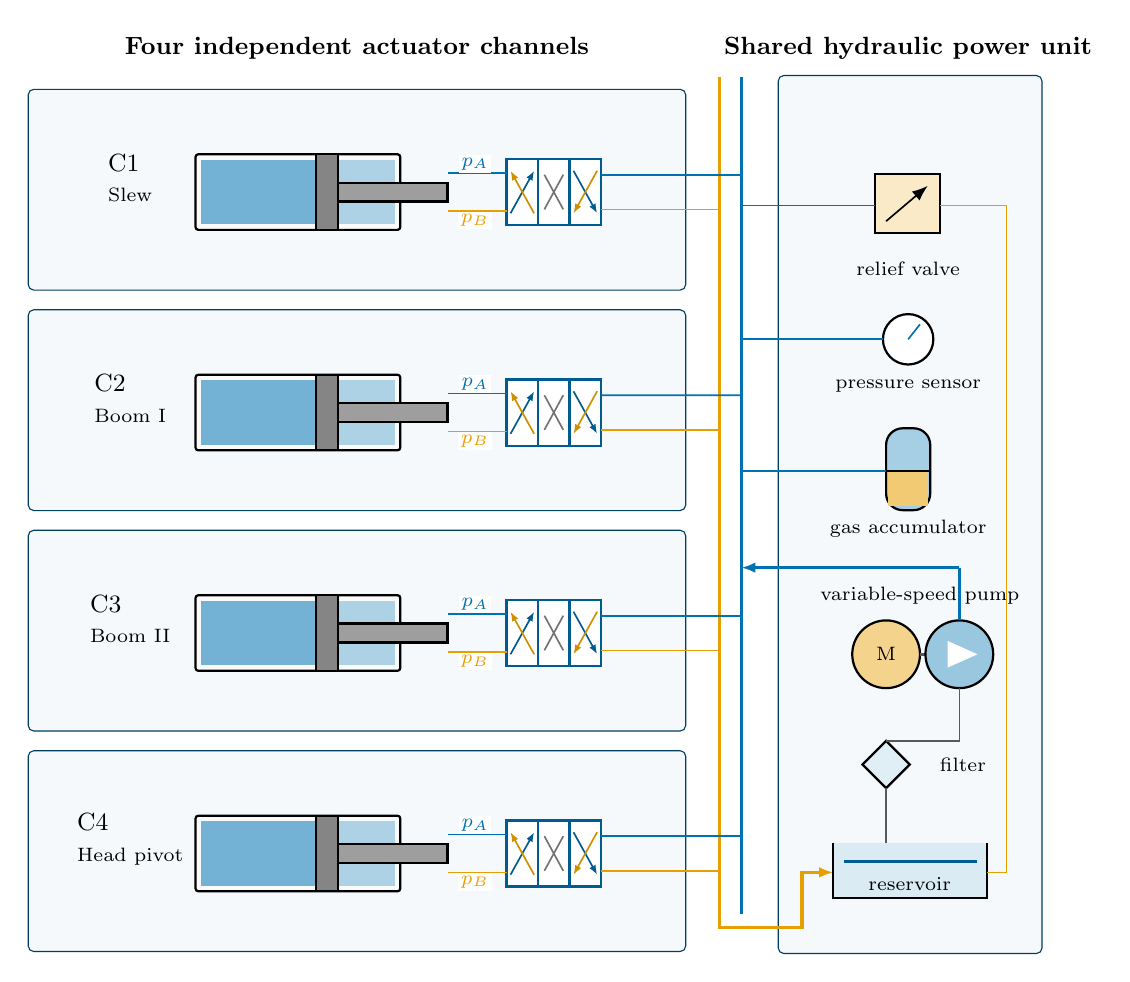
\begin{tikzpicture}[x=1cm,y=1cm,>=Latex,font=\footnotesize]
    \tikzset{hydchannel/.style={draw=cbblue!55!black,rounded corners=2pt,fill=cbblue!4,
      minimum width=8.35cm,minimum height=2.55cm}}
    % Reusable ISO-inspired cylinder and 4/3 directional-valve symbols.
    \newcommand{\hydcylinder}[1]{%
      \draw[thick,rounded corners=1pt,fill=black!2] (2.05,#1-.48) rectangle (4.65,#1+.48);
      \fill[cbblue!55] (2.12,#1-.41) rectangle (3.58,#1+.41);
      \fill[cbblue!32] (3.86,#1-.41) rectangle (4.58,#1+.41);
      \draw[thick,fill=black!48] (3.58,#1-.48) rectangle (3.86,#1+.48);
      \draw[thick,fill=black!38] (3.86,#1-.12) rectangle (5.25,#1+.12);
    }
    \newcommand{\dcvalve}[2]{%
      \draw[draw=cbblue!80!black,fill=white,thick] (6.00,#2-.42) rectangle (7.20,#2+.42);
      \draw[cbblue!80!black,thick] (6.40,#2-.42) -- (6.40,#2+.42);
      \draw[cbblue!80!black,thick] (6.80,#2-.42) -- (6.80,#2+.42);
      \draw[cbblue!80!black,semithick,-{Latex[length=1.2mm]}] (6.05,#2-.27) -- (6.35,#2+.27);
      \draw[cborange!90!black,semithick,-{Latex[length=1.2mm]}] (6.35,#2-.27) -- (6.05,#2+.27);
      \draw[black!55,semithick] (6.48,#2-.22) -- (6.72,#2+.22);
      \draw[black!55,semithick] (6.48,#2+.22) -- (6.72,#2-.22);
      \draw[cbblue!80!black,semithick,-{Latex[length=1.2mm]}] (6.85,#2+.27) -- (7.15,#2-.27);
      \draw[cborange!90!black,semithick,-{Latex[length=1.2mm]}] (7.15,#2+.27) -- (6.85,#2-.27);
      \draw[cbblue,semithick] (5.25,#2+.24) -- (6.00,#2+.24);
      \draw[cborange,semithick] (5.25,#2-.24) -- (6.00,#2-.24);
      \coordinate (v#1s) at (7.20,#2+.22);
      \coordinate (v#1t) at (7.20,#2-.22);
    }
    \node[font=\small\bfseries] at (4.1,.45) {Four independent actuator channels};
    \node[font=\small\bfseries] at (11.1,.45) {Shared hydraulic power unit};

    \node[hydchannel] at (4.1,-1.35) {};
    \node[hydchannel] at (4.1,-4.15) {};
    \node[hydchannel] at (4.1,-6.95) {};
    \node[hydchannel] at (4.1,-9.75) {};
    \draw[draw=cbblue!55!black,rounded corners=2pt,fill=cbblue!4] (9.45,.1) rectangle (12.8,-11.05);

    % Common supply and return rails
    \draw[cborange,very thick] (8.7,.08) -- (8.7,-10.55);
    \draw[cbblue,very thick] (8.98,.08) -- (8.98,-10.55);

    % C1
    \node[align=left,font=\small] at (1.22,-1.2) {C1\\\scriptsize Slew};
    \hydcylinder{-1.38}
    \dcvalve{1}{-1.38}
    \draw[cbblue,semithick] (v1s) -- (8.98,-1.16);
    \draw[cborange,semithick] (v1t) -- (8.7,-1.60);
    \node[font=\scriptsize,cbblue,fill=white,inner sep=1pt] at (5.60,-1.02) {$p_A$};
    \node[font=\scriptsize,cborange,fill=white,inner sep=1pt] at (5.60,-1.74) {$p_B$};

    % C2
    \node[align=left,font=\small] at (1.22,-4.0) {C2\\\scriptsize Boom I};
    \hydcylinder{-4.18}
    \dcvalve{2}{-4.18}
    \draw[cbblue,semithick] (v2s) -- (8.98,-3.96);
    \draw[cborange,semithick] (v2t) -- (8.7,-4.40);
    \node[font=\scriptsize,cbblue,fill=white,inner sep=1pt] at (5.60,-3.82) {$p_A$};
    \node[font=\scriptsize,cborange,fill=white,inner sep=1pt] at (5.60,-4.54) {$p_B$};

    % C3
    \node[align=left,font=\small] at (1.22,-6.8) {C3\\\scriptsize Boom II};
    \hydcylinder{-6.98}
    \dcvalve{3}{-6.98}
    \draw[cbblue,semithick] (v3s) -- (8.98,-6.76);
    \draw[cborange,semithick] (v3t) -- (8.7,-7.20);
    \node[font=\scriptsize,cbblue,fill=white,inner sep=1pt] at (5.60,-6.62) {$p_A$};
    \node[font=\scriptsize,cborange,fill=white,inner sep=1pt] at (5.60,-7.34) {$p_B$};

    % C4
    \node[align=left,font=\small] at (1.22,-9.6) {C4\\\scriptsize Head pivot};
    \hydcylinder{-9.78}
    \dcvalve{4}{-9.78}
    \draw[cbblue,semithick] (v4s) -- (8.98,-9.56);
    \draw[cborange,semithick] (v4t) -- (8.7,-10.00);
    \node[font=\scriptsize,cbblue,fill=white,inner sep=1pt] at (5.60,-9.42) {$p_A$};
    \node[font=\scriptsize,cborange,fill=white,inner sep=1pt] at (5.60,-10.14) {$p_B$};

    % Power unit
    \draw[thick,fill=cbblue!14] (10.15,-9.65) -- (10.15,-10.35) -- (12.1,-10.35) -- (12.1,-9.65);
    \draw[cbblue!80!black,very thick] (10.28,-9.88) -- (11.97,-9.88);
    \node[font=\scriptsize] at (11.12,-10.17) {reservoir};
    \draw[thick,fill=cbblue!12] (10.52,-8.65) -- (10.82,-8.35) -- (11.12,-8.65) -- (10.82,-8.95) -- cycle;
    \node[font=\scriptsize,anchor=west] at (11.38,-8.65) {filter};
    \draw[fill=cborange!45,thick] (10.82,-7.25) circle (.43);
    \node[font=\scriptsize] at (10.82,-7.25) {M};
    \draw[black!65,line width=1.2pt] (11.25,-7.25) -- (11.32,-7.25);
    \draw[fill=cbblue!40,thick] (11.75,-7.25) circle (.43);
    \fill[white] (11.60,-7.42) -- (11.60,-7.08) -- (11.98,-7.25) -- cycle;
    \node[font=\scriptsize] at (11.25,-6.5) {variable-speed pump};
    \draw[thick,rounded corners=6pt,fill=cbblue!35] (10.82,-5.42) rectangle (11.38,-4.38);
    \fill[cborange!55] (10.85,-5.37) rectangle (11.35,-4.92);
    \draw[thick] (10.82,-4.92) -- (11.38,-4.92);
    \node[font=\scriptsize] at (11.1,-5.65) {gas accumulator};
    \draw[thick,fill=white] (11.1,-3.25) circle (.32);
    \draw[cbblue,semithick] (11.1,-3.25) -- (11.25,-3.06);
    \node[font=\scriptsize] at (11.1,-3.85) {pressure sensor};
    \draw[thick,fill=cborange!22] (10.68,-1.9) rectangle (11.5,-1.15);
    \draw[->,semithick] (10.82,-1.75) -- (11.35,-1.3);
    \node[font=\scriptsize] at (11.1,-2.35) {relief valve};
    % The suction path is kept below the pump; the pressure path leaves from
    % the pump top. This avoids crossing the motor, pump, filter, and reservoir.
    \draw[black!65,semithick] (10.82,-9.65) -- (10.82,-8.95);
    \draw[black!65,semithick] (10.82,-8.35) -| (11.75,-7.68);
    \draw[cbblue,very thick] (11.75,-6.82) -- (11.75,-6.15);
    \draw[cbblue,very thick,-{Latex[length=1.8mm]}] (11.75,-6.15) -- (8.98,-6.15);
    \draw[cbblue,semithick] (8.98,-4.92) -- (10.82,-4.92);
    \draw[cbblue,semithick] (8.98,-3.25) -- (10.78,-3.25);
    \draw[cbblue,semithick] (8.98,-1.55) -- (10.68,-1.55);
    \draw[cborange,semithick] (11.50,-1.55) -- (12.35,-1.55) -- (12.35,-10.02) -- (12.1,-10.02);
    \draw[cborange,very thick,-{Latex[length=1.8mm]}]
      (8.7,-10.35) -- (8.7,-10.72) -- (9.75,-10.72) -- (9.75,-10.02) -- (10.15,-10.02);
  \end{tikzpicture}%
  }
  \caption{Hydraulic system schematic. Four proportional-valve cylinder
  channels share a variable-speed pump, reservoir, accumulator, sensor, and
  pressure-relief valve. Blue and orange rails denote supply and return.}
  \label{fig:sys:schematic}
\end{figure}

Figure~\ref{fig:sys:actuator-channel} identifies the cylinder chambers,
piston, seal, and rod used in the actuator model.

\begin{figure}[htbp]
  \centering
  \begin{tikzpicture}
    \node[inner sep=0] (cylinder) {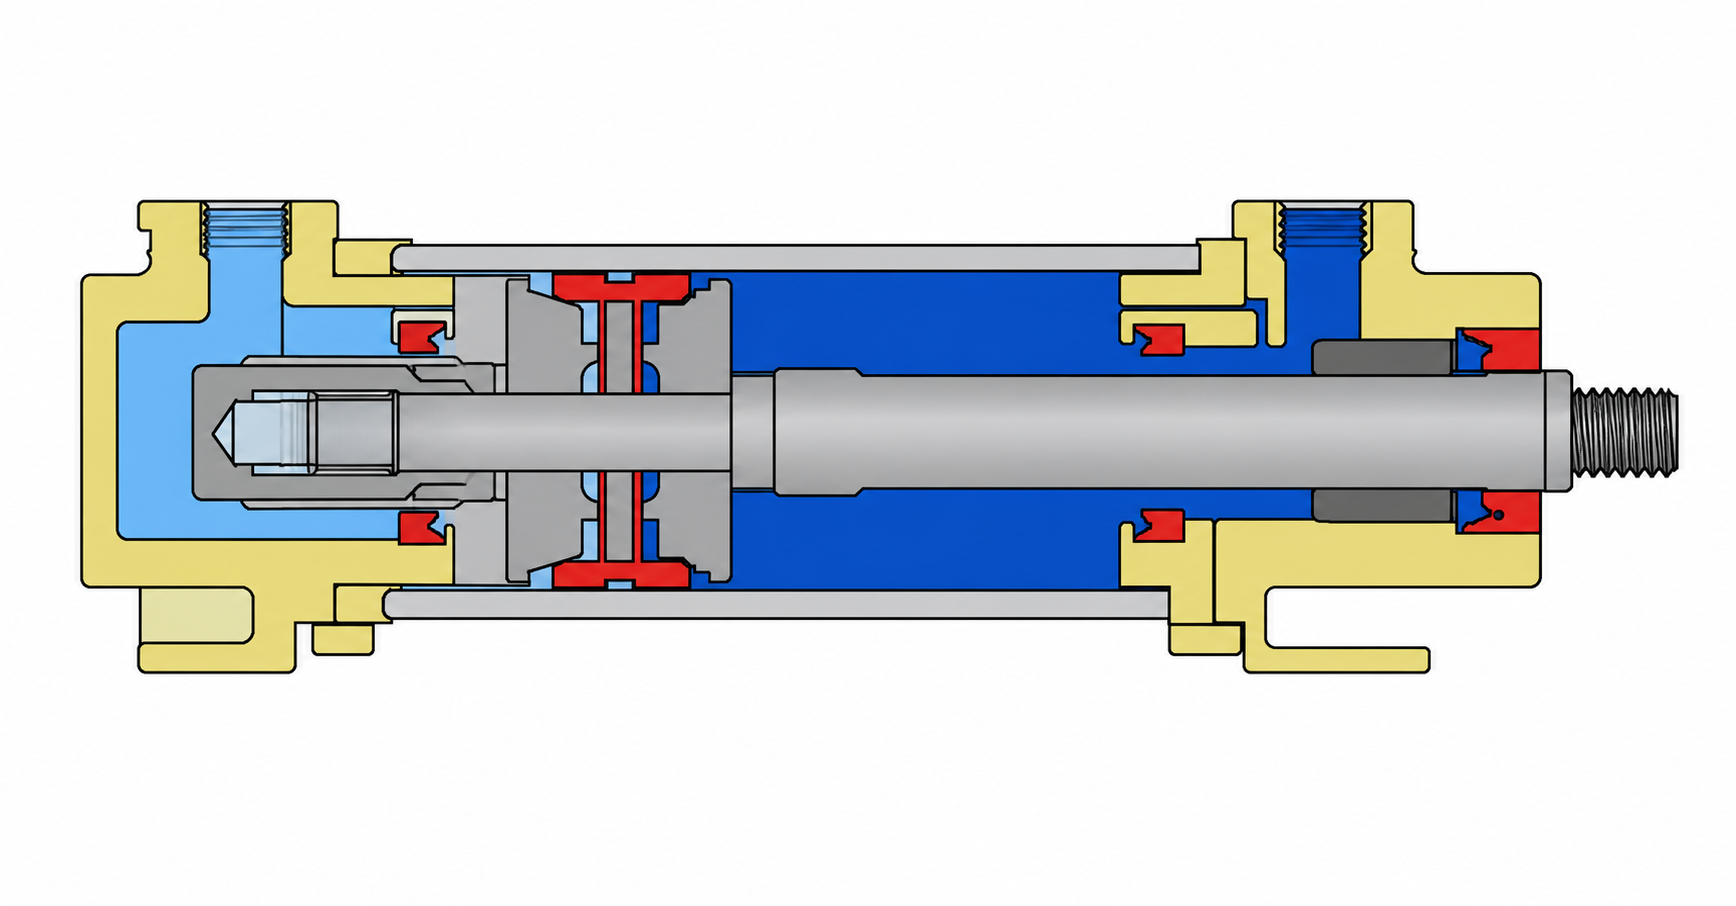
\includegraphics[width=.98\textwidth]{images/ch3_double_acting_cylinder_cutaway}};
    % Color-coded callouts follow the electrical--hydraulic--mechanical
    % annotation language used in Figure~\ref{fig:fund:chain}.
    \node[draw=cbblue,fill=white,rounded corners=1pt,inner sep=3pt,font=\normalsize,anchor=north west] (caplabel)
      at ([xshift=2mm,yshift=-2mm]cylinder.north west) {Cap-side chamber ($p_A,Q_A$)};
    \node[draw=cbgreen,fill=white,rounded corners=1pt,inner sep=3pt,font=\normalsize,anchor=north] (pistonlabel)
      at ([xshift=-18mm,yshift=-2mm]cylinder.north) {Piston};
    \node[draw=cbgreen,fill=white,rounded corners=1pt,inner sep=3pt,font=\normalsize,anchor=north] (seallabel)
      at ([xshift=12mm,yshift=-2mm]cylinder.north) {Piston seal};
    \node[draw=cbblue,fill=white,rounded corners=1pt,inner sep=3pt,font=\normalsize,anchor=north east] (rodlabel)
      at ([xshift=-2mm,yshift=-2mm]cylinder.north east) {Rod-side chamber ($p_B,Q_B$)};
    \node[draw=cbgreen,fill=white,rounded corners=1pt,inner sep=3pt,font=\normalsize,anchor=south east] (strokelabel)
      at ([xshift=-2mm,yshift=2mm]cylinder.south east) {Piston rod; stroke $x$};
    \draw[cbblue,semithick,-{Latex[length=1.8mm]}] (caplabel.south east) --
      ([xshift=15mm,yshift=-36mm]cylinder.north west);
    \draw[cbgreen,semithick,-{Latex[length=1.8mm]}] (pistonlabel.south) --
      ([xshift=-17mm,yshift=-42mm]cylinder.north);
    \draw[cbgreen,semithick,-{Latex[length=1.8mm]}] (seallabel.south) --
      ([xshift=-14mm,yshift=-26mm]cylinder.north);
    \draw[cbblue,semithick,-{Latex[length=1.8mm]}] (rodlabel.south west) --
      ([xshift=-60mm,yshift=-29mm]cylinder.north east);
    \draw[cbgreen,semithick,-{Latex[length=1.8mm]}] (strokelabel.north west) --
      ([xshift=-38mm,yshift=39mm]cylinder.south east);
  \end{tikzpicture}
  \caption{Annotated cutaway of an asymmetric double-acting hydraulic
  cylinder. The cap-side and rod-side chamber pressures generate the piston
  force and rod stroke.}
  \label{fig:sys:actuator-channel}
\end{figure}

The 4/3 valve in Figure~\ref{fig:sys:schematic} meters flow to the cylinder
chambers. The
chamber pressures follow
%
\begin{equation}
  \label{eq:sys:continuity}
  \dot{p}_1 = \frac{E_{\mathrm{eff}}}{V_1(x)}
    \bigl( Q_1 - A_1 \dot{x} - C_{\mathrm{leak}}(p_1 - p_2) \bigr),
  \qquad
  \dot{p}_2 = \frac{E_{\mathrm{eff}}}{V_2(x)}
    \bigl( -Q_2 + A_2 \dot{x} + C_{\mathrm{leak}}(p_1 - p_2) \bigr),
\end{equation}
%
where $V_{1,2}(x)$ include dead volumes, $A_1\neq A_2$, and
$C_{\mathrm{leak}}$ is internal leakage. Entrained air is represented by
%
\begin{equation}
  \label{eq:sys:bulk}
  E_{\mathrm{eff}}(p) =
  \left( \frac{1}{E_f} + \frac{\alpha}{p} \right)^{-1},
\end{equation}
%
Valve flow follows the orifice law of
Section~\ref{sec:fund:actuation-chain}; spool dynamics are
$\dot{x}_v=(u-x_v)/\tau_v$. The piston force is
$F_h=p_1A_1-p_2A_2-F_{\mathrm{fric}}(\dot{x})$. The coupled model is stiff and
uses a variable-step implicit solver, which prevents RL-time simulation.

\subsection{Validated Scope of the Model}
\label{sec:sys:simscape-validation}

Validation uses a fixed integral-backstepping controller at $\unit[0.01]{s}$
while sweeping $\beta\in\{0.5,1.0,1.5,2.0\}\,\mathrm{GPa}$. Slew-axis delay
falls from about $\unit[0.85]{s}$ to $\unit[0.65]{s}$, the system delay index
from $\unit[0.45]{s}$ to $\unit[0.35]{s}$, and task-space tracking error by
about 11\,\%. The improvement saturates beyond $\unit[1.5]{GPa}$.

The model represents one machine, omits thermal dynamics, and treats the logged
rod-force channel as unreliable after the piston-area consistency audit
(Section~\ref{sec:models:rom}). Chapter~\ref{chap:data} introduces variation
through parameter randomization.

\section{IsaacLab Environment}
\label{sec:sys:isaaclab}

Policy training, adaptation-data collection, and evaluation run in
IsaacLab~\cite{mittal2023orbit} on PhysX. The USD articulation contains the
Unimog carrier, five arm links, and four prismatic cylinder joints. Learned
actuator models supply the hydraulic behavior between the controller and PhysX
cylinder targets.

\subsection{Simulation and Control Rates}
\label{sec:sys:timing}

Table~\ref{tab:sys:rates} lists the four simulation clocks. PhysX runs at
$\unit[120]{Hz}$ and the policy at $\unit[60]{Hz}$. The learned actuator models
and AAM update every three policy steps ($\unit[0.05]{s}$); their prediction is
held across the intervening PhysX updates. Data collection uses this same
$\unit[50]{ms}$ grid.

\begin{table}[htbp]
  \centering
  \caption{The four rates of the simulated system. They are reported
  separately throughout the thesis; ``the control frequency'' is not a
  well-defined quantity here.}
  \label{tab:sys:rates}
  \small
  \begin{tabular}{lll}
    \toprule
    Layer & Step & Rate \\
    \midrule
    PhysX physics                & $\unit[1/120]{s}$   & $\unit[120]{Hz}$ \\
    Policy / control (decimation 2) & $\unit[1/60]{s}$ & $\unit[60]{Hz}$ \\
    Learned actuator model (3 control steps) & $\unit[0.05]{s}$ & $\unit[20]{Hz}$ \\
    AAM latent update            & $\unit[0.05]{s}$    & $\unit[20]{Hz}$ \\
    \bottomrule
  \end{tabular}
\end{table}

\subsection{Environment Configuration Details}

The arm root is spawned at $z=\unit[1.26]{m}$; ground-height spawning buries
the vehicle. Cylinder targets are integrated in reference space so gravity does
not erase commanded increments. Vehicle motion is scripted because the authored
tyres and suspension do not provide reliable PhysX traction; a planar fixture
holds lateral position and heading.

\section{The Verge-Following Task}
\label{sec:sys:task}

\subsection{Task Definition}

The task is moving verge following. The truck drives a $\unit[26]{m}$ strip at
a speed sampled from $2$ to $\unit[7]{km/h}$; development uses
$\unit[4]{km/h}$. Episodes allow $2808$ steps ($\unit[46.8]{s}$), while scoring
stops when the strip is completed. The arm must keep the cutter at the target
height, on the verge centre line, in contact with the ground, and within its
travel limits. Terrain height is randomized per environment
(Figure~\ref{fig:sys:verge-task-render}).

\begin{figure}[htbp]
  \centering
  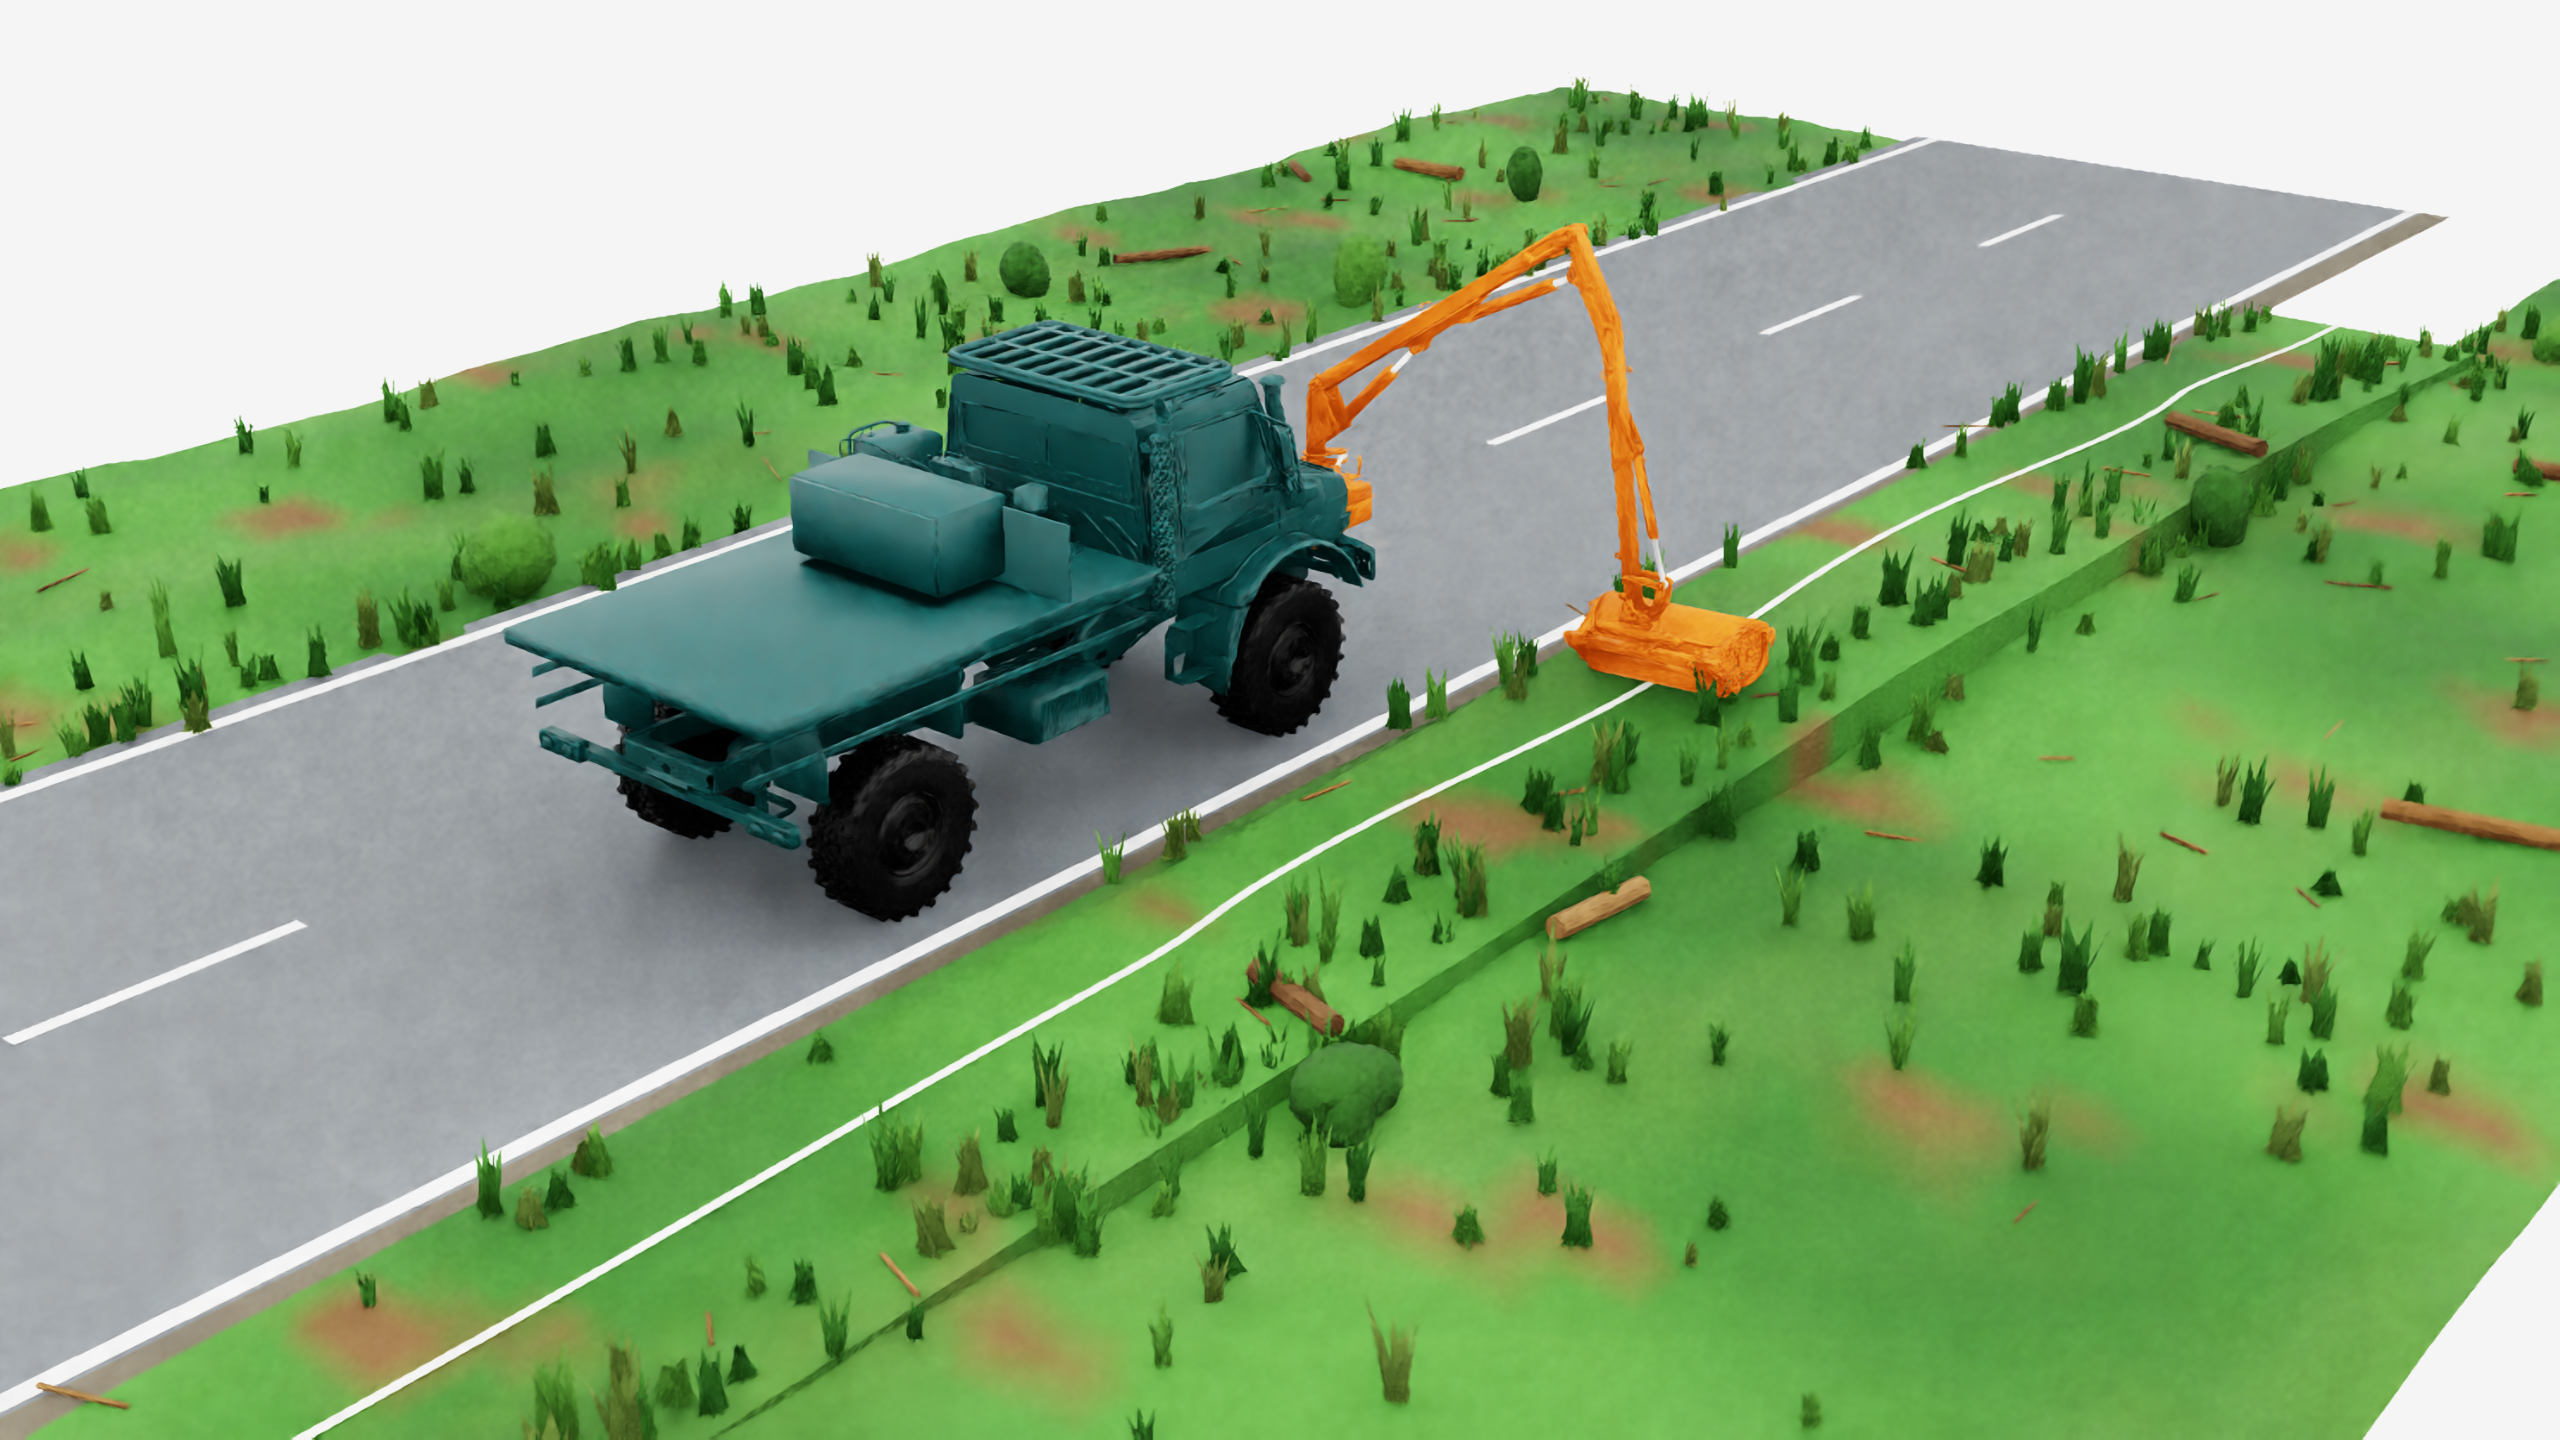
\includegraphics[width=\textwidth]{images/ch3_verge_task_render.png}
  \caption{IsaacLab realization of the moving verge-following task. The
  scripted truck travels on the level road while the four-cylinder arm places
  the cutter above the procedurally generated verge and follows the white
  reference path. Randomized grass, bushes, soil patches, twigs, and logs form
  a non-colliding visual layer; the underlying verge mesh supplies the terrain
  disturbance and height-sensing geometry used by the controller.}
  \label{fig:sys:verge-task-render}
\end{figure}

Eleven reference-path families span straight, periodic, spline, sweep, and
lane-change motion. Results use the worst path family and terrain mesh rather
than a pooled score. A regression test verifies that all eleven families are
distinct.

\subsection{Task Feasibility and Plant Capability}
\label{sec:sys:capability}

The action contract limits cylinders~1--3 to $\unit[4]{mm}$ per policy step,
which bounds lateral cutter speed at
%
\begin{equation}
  \label{eq:sys:rate-ceiling}
  v_{\mathrm{lat}}^{\max}
  = \frac{\unit[4]{mm}}{\unit[1/60]{s}} = \unit[0.240]{m/s}.
\end{equation}
%
This uses the $\unit[1/60]{s}$ policy interval. Early path settings exceeded
this limit; the worst case (\texttt{boom\_sweep}) required $3.7\times$ the
available rate. Path and terrain parameters are now derived from
\eqref{eq:sys:rate-ceiling}, and a preflight check rejects infeasible tasks.

\section{Control Architecture}
\label{sec:sys:architecture}

\begin{figure}[t]
  \centering
  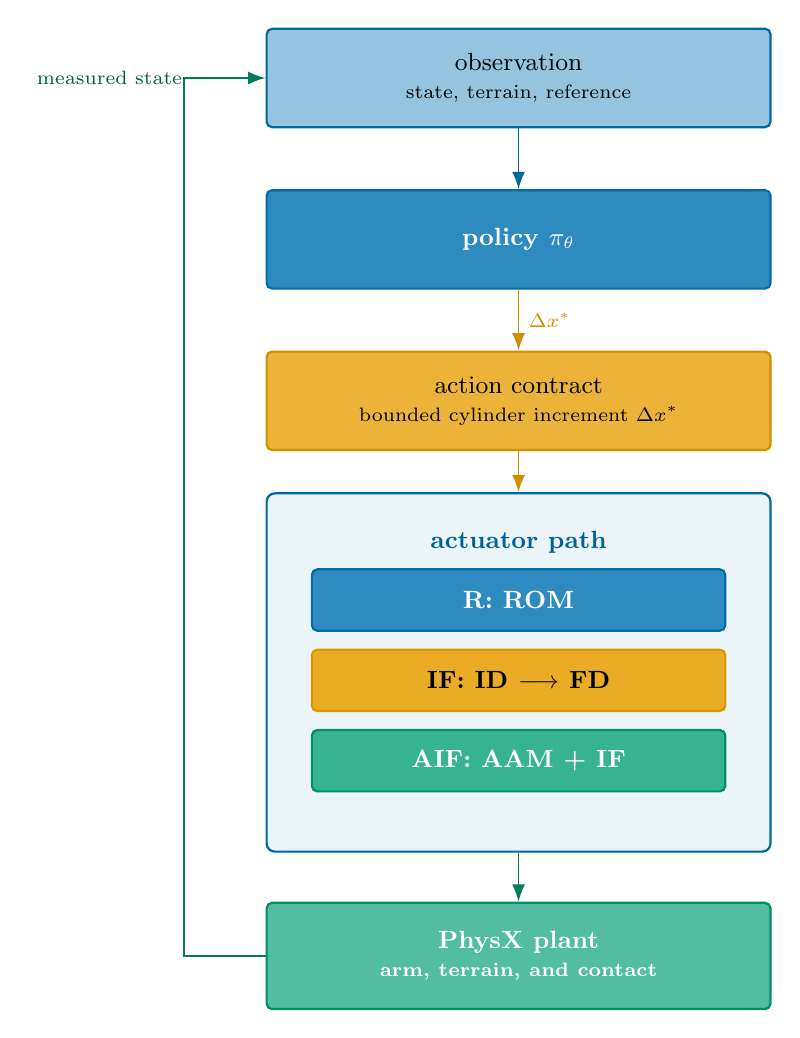
\begin{tikzpicture}[x=1cm,y=1cm,>=Latex,font=\small]
    \node[draw=cbblue!90!black,line width=.8pt,rounded corners=2pt,fill=cbblue!42,
      minimum width=6.4cm,minimum height=1.25cm,align=center,font=\small] (obs) at (0,0)
      {observation\\[-1pt]\scriptsize state, terrain, reference};
    \node[draw=cbblue!95!black,line width=.8pt,rounded corners=2pt,fill=cbblue!82,text=white,
      minimum width=6.4cm,minimum height=1.25cm,align=center,font=\small\bfseries] (policy) at (0,-2.05)
      {policy $\pi_\theta$};
    \node[draw=cborange!90!black,line width=.8pt,rounded corners=2pt,fill=cborange!78,
      minimum width=6.4cm,minimum height=1.25cm,align=center,font=\small] (contract) at (0,-4.1)
      {action contract\\[-1pt]\scriptsize bounded cylinder increment $\Delta x^*$};

    \node[draw=cbblue!90!black,line width=.8pt,rounded corners=3pt,fill=cbblue!8,minimum width=6.4cm,
      minimum height=4.55cm] (path) at (0,-7.55) {};
    \node[font=\small\bfseries,text=cbblue!85!black] at (0,-5.9) {actuator path};
    \node[draw=cbblue!95!black,line width=.8pt,rounded corners=2pt,fill=cbblue!82,text=white,
      minimum width=5.25cm,minimum height=.78cm,font=\small\bfseries] at (0,-6.63) {R: ROM};
    \node[draw=cborange!95!black,line width=.8pt,rounded corners=2pt,fill=cborange!86,
      minimum width=5.25cm,minimum height=.78cm,font=\small\bfseries] at (0,-7.65)
      {IF: ID $\longrightarrow$ FD};
    \node[draw=cbgreen!90!black,line width=.8pt,rounded corners=2pt,fill=cbgreen!78,text=white,
      minimum width=5.25cm,minimum height=.78cm,font=\small\bfseries] at (0,-8.67)
      {AIF: AAM + IF};

    \node[draw=cbgreen!90!black,line width=.8pt,rounded corners=2pt,fill=cbgreen!68,text=white,
      minimum width=6.4cm,minimum height=1.35cm,align=center,font=\small\bfseries] (plant) at (0,-11.15)
      {PhysX plant\\[-1pt]\scriptsize arm, terrain, and contact};

    \draw[sigarrow,cbblue!90!black] (obs) -- (policy);
    \draw[sigarrow,cborange!90!black] (policy) -- (contract)
      node[midway,right,font=\scriptsize] {$\Delta x^*$};
    \draw[sigarrow,cborange!90!black] (contract) -- (path.north);
    \draw[sigarrow,cbgreen!80!black] (path.south) -- (plant);
    \draw[sigarrow,cbgreen!80!black] (plant.west) -| (-4.25,-11.15) |- (obs.west)
      node[pos=.55,left,font=\scriptsize,text=cbgreen!60!black] {measured state};
  \end{tikzpicture}
  \caption{Deployed control stack. The policy produces a bounded cylinder
  increment; R, IF, or AIF realizes it in the shared PhysX plant. Measured
  state closes the loop.}
  \label{fig:sys:architecture}
\end{figure}

The vehicle advances at the scripted speed and the reference generator supplies
the verge centre line and cut height. The policy maps normalized observations to
four desired cylinder increments; it has no runtime baseline controller. The
action contract bounds those increments. R uses the command ROM, IF the frozen
inverse/forward pair, and AIF adds the bounded adapter conditioned on
$\latenthat$. All paths set the same PhysX cylinder target. The DLS controller
is used only for teaching and identification.

\section{Problem Formulation}
\label{sec:sys:problem}

The reference is the verge centre line $y_{\mathrm{ref}}(t)$ and cut height
$h_{\mathrm{ref}}$, expressed in the truck frame. With cutter-tip position
$\bm{p}_c(t)$ and terrain height $g(\cdot)$, the scored errors are
%
\begin{equation}
  \label{eq:sys:error}
  e_{\mathrm{lat}}(t) = p_{c,y}(t) - y_{\mathrm{ref}}(t),
  \qquad
  e_{\mathrm{cut}}(t)
    = \bigl(p_{c,z}(t) - g(\bm{p}_c(t))\bigr) - h_{\mathrm{ref}} .
\end{equation}
%
The objective is to minimize the mean and tail of both errors across path
families and terrain while maintaining contact, head alignment, and smooth
motion. Learned models are evaluated on one-step and recursive cylinder
predictions. The stacks are tested across the randomized plant family; AIF is
compared with IF on held-out factors.

Constraints are cylinder limits and headroom
(Table~\ref{tab:sys:cylinders}), the action contract, checkpoint output limits,
and the head-down condition.

\section{System-Level Evaluation Criteria}
\label{sec:sys:evaluation-criteria}

Controllers and models are evaluated separately. Controller scores can hide
actuator-model errors through policy compensation.

The system-level criteria cover three aspects of operation. Cut-height and
lateral errors measure task accuracy. Contact, head alignment, impact rate,
and cutter acceleration describe tool--terrain interaction and motion quality.
Cylinder headroom and safety terminations check whether the task is completed
without driving the mechanism into its limits. The metrics are evaluated over
the scored part of each episode and are kept in physical units where possible.
This makes a failed gate traceable to a specific limitation rather than to a
single combined reward value.

\subsection{Eight-Gate Acceptance Contract}
\label{sec:sys:gates}

Table~\ref{tab:sys:gates} defines the system-level acceptance contract.

All controller stacks are evaluated with the same path, terrain, and
randomization conditions. A stack passes only when it satisfies every gate;
strong mean tracking cannot compensate for loss of contact, inadequate
cylinder headroom, excessive impacts, or safety terminations. Worst-case
aggregation prevents easy terrain or path cases from masking a local failure.
Mean absolute errors quantify sustained tracking performance, while the lower
and upper percentiles capture short alignment, clearance, or acceleration
events that a mean can hide. Contact and termination measures are reported as
fractions so that episodes of different completed length remain comparable.

\begin{table}[htbp]
  \centering
  \caption{Eight system-level acceptance gates. Each gate uses at least three
  terrain meshes and the worst mesh; tracking-critical gates also use the worst
  path family. $^{\dagger}$Hard impacts is a wear constraint.}
  \label{tab:sys:gates}
  \small
  \begin{tabular}{llll}
    \toprule
    Gate & Metric & Threshold & Aggregation \\
    \midrule
    Cut height        & mean $|e_{\mathrm{cut}}|$
                      & $\leq \unit[0.040]{m}$ & worst mesh \\
    Lateral tracking  & mean $|e_{\mathrm{lat}}|$
                      & $\leq \unit[0.300]{m}$ & worst mesh, worst family \\
    Ground contact    & contact fraction
                      & $\geq 0.700$ & worst mesh, worst family \\
    Head alignment    & p01 head-down alignment
                      & $\geq 0.900$ & worst mesh \\
    Hard impacts$^{\dagger}$ & hard-impact step fraction
                      & $\leq 0.350$ & worst mesh \\
    Tool acceleration & p95 cutter acceleration
                      & $\leq \unit[120]{m/s^2}$ & worst mesh \\
    Cylinder headroom & p01 travel margin
                      & $\geq \unit[0.005]{m}$ & worst mesh \\
    Safety terminations & termination rate
                      & $\leq 0.080$ & worst mesh \\
    \bottomrule
  \end{tabular}
\end{table}

\subsection{Cylinder and Model Checks}

Cylinder checks use fresh $\pm\unit[10]{mm}$ commands, coordinated
$\unit[80]{mm}$ motions, return error, and saturation. Model checks use
one-step and rollout accuracy, input ablation, and Jacobian conditioning
(Chapter~\ref{chap:models}). Chapter~\ref{chap:evaluation} reports these with
the acceptance contract. The small command checks local response and deadband;
the coordinated motion checks coupling between actuator channels. Return error
tests reversibility, and saturation checks whether the learned model respects
the command and stroke limits. These diagnostics are interpreted alongside the
system gates, not as substitutes for closed-loop task performance.

The system is now specified. The next chapter turns to the data the learned
models are built from.

\RRLABchapterblank
%%%%%%%%%%%%%%%%%%%%%%%%%%%%%%%%%%%%%%%%%%%%%%%%%%%%%%%%%%%%
%% Chapter 4 - Data Generation and Preparation (10-16 pages)
%% Purpose: explain how the Simscape datasets were designed to
%% contain realistic operation, causal actuator excitation, and
%% variation required for robust and adaptive learning.
%%%%%%%%%%%%%%%%%%%%%%%%%%%%%%%%%%%%%%%%%%%%%%%%%%%%%%%%%%%%
\chapter{Data Generation and Preparation}
\label{chap:data}

Chapter~\ref{chap:system} defined two plant representations: detailed
hydraulics in Simscape and fast rigid-body dynamics in IsaacLab. This chapter
documents the datasets that connect them, including collection, auditing,
feature construction and splitting. Table~\ref{tab:sys:provenance} records
their provenance.

\emph{Simscape campaigns.} Closed-loop runs provide realistic operating data
for the inverse and reduced-order models. Separate open-loop valve excitation
provides the causal command information needed by the strict forward model
(Section~\ref{sec:data:open-loop}).

\emph{ROM calibration.} After Simscape training, the command ROM was
fine-tuned on five closed-loop IsaacLab reference shapes. Only its bounded
correction head remained trainable, with Simscape replay retained
(Section~\ref{sec:data:rom-calibration}). The ID--FD pair was not calibrated
in IsaacLab.

\emph{IsaacLab deployment data.} The system-dynamics surrogate, the privileged
encoder and the adaptation module use two $118$-run collections recorded in the
deployed command
ROM--PhysX plant, including dedicated PRBS windows
(Section~\ref{sec:data:isaaclab}). No earlier adaptation or system-dynamics
model was reused. Figure~\ref{fig:data:pipeline} summarises the common
preparation workflow.

\begin{figure}[p]
  \centering
  \begin{tikzpicture}[x=1cm,y=1cm,>=Latex,font=\small,
    source/.style={draw=black!55,line width=.8pt,rounded corners=2pt,
      fill=white,minimum width=3.05cm,minimum height=1.25cm,
      align=center,inner sep=3pt},
    process/.style={draw=black!55,line width=.8pt,rounded corners=2pt,
      fill=white,minimum width=5.4cm,minimum height=1.08cm,
      align=center,font=\small},
    output/.style={draw=black!65,line width=.8pt,rounded corners=2pt,
      fill=white,minimum width=3.05cm,minimum height=1.35cm,
      align=center,font=\small},
    stage/.style={circle,draw=black!70,fill=white,text=black,
      line width=.8pt,minimum size=7mm,inner sep=0pt,font=\small\bfseries},
    flow/.style={-{Latex[length=2.2mm]},line width=.8pt,draw=black!75},
    bus/.style={line width=.8pt,draw=black!65}]

    \node[font=\large\bfseries,text=black!80] at (0,.65) {DATA COLLECTION};
    \draw[black!40] (-6.95,.25) -- (6.95,.25);
    \node[font=\small\bfseries,text=black!80] at (-3.50,-.12) {SIMSCAPE};
    \node[font=\small\bfseries,text=black!80] at (3.50,-.12)
      {ISAACLAB / DEPLOYMENT};
    \node[draw=black!60,line width=.7pt,rounded corners=5pt,
      fill=white,minimum width=6.25cm,minimum height=.48cm,
      font=\scriptsize,text=black!75] at (-3.50,-.67)
      {\textbf{Randomised campaign}\quad $1\,000$ runs $\cdot$ $12$ parameters};

    \node[source] (closed) at (-5.25,-1.85)
      {\textbf{Closed-loop}\\[-1pt]\footnotesize $1\,040$ runs};
    \node[source] (open) at (-1.75,-1.85)
      {\textbf{Open-loop}\\[-1pt]\footnotesize $4$ runs};
    \node[source] (romsrc) at (1.75,-1.85)
      {\textbf{ROM calibration}\\[-1pt]\footnotesize $5$ references};
    \node[source] (adapt) at (5.25,-1.85)
      {\textbf{Adaptation data}\\[-1pt]\footnotesize $118$ runs};
    \coordinate (collectbus) at (0,-2.85);
    \foreach \s in {closed,open,romsrc,adapt}{
      \draw[line width=.8pt,black!70] (\s.south) -- (\s.south |- collectbus);}
    \draw[line width=.8pt,black!70] (-5.25,-2.85) -- (5.25,-2.85);

    \node[process] (extract) at (0,-3.90)
      {\textbf{EXTRACT \& ALIGN}\\[-1pt]\footnotesize states $\bullet$ actions $\bullet$ targets};
    \node[stage] at (-3.25,-3.90) {1};
    \draw[flow] (collectbus) -- (extract.north);

    \node[diamond,aspect=2.15,draw=black!75,line width=.9pt,
      fill=black!12,align=center,inner sep=2pt,font=\footnotesize\bfseries]
      (audit) at (0,-5.90)
      {QUALITY AUDIT\\[-1pt]\scriptsize validity $\bullet$ excitation};
    \node[stage] at (-3.25,-5.90) {2};
    \draw[flow] (extract.south) -- (audit.north);

    \node[draw=rltred,line width=1.5pt,rounded corners=2pt,
      fill=rltred!10,minimum width=2.80cm,minimum height=1.10cm,
      align=center,font=\footnotesize\bfseries] (recollect) at (5.55,-5.90)
      {RECOLLECT\\[-1pt]OR REDESIGN};
    \draw[-{Latex[length=2.2mm]},line width=1.3pt,rltred]
      (audit.east) -- (recollect.west);
    \node[anchor=south,fill=white,inner sep=1pt,
      font=\scriptsize\bfseries,text=rltred]
      at ($(audit.east)!.50!(recollect.west)+(0,1.7mm)$) {FAIL};
    \draw[-{Latex[length=2.0mm]},line width=1.0pt,dashed,rltred]
      (recollect.east) |- (5.25,-2.85);

    \node[process,draw=rltgreen,fill=rltgreen!10,line width=1.5pt]
      (split) at (0,-8.20)
      {\textbf{SPLIT BY RUN}\\[-1pt]\footnotesize train $\bullet$ validation $\bullet$ test};
    \node[stage] at (-3.25,-8.20) {3};
    \draw[-{Latex[length=2.2mm]},line width=1.3pt,rltgreen]
      (audit.south) -- (split.north);
    \node[anchor=west,fill=white,inner sep=1pt,
      font=\scriptsize\bfseries,text=rltgreen]
      at ($(audit.south)!.38!(split.north)+(4.0mm,0)$) {PASS};

    \node[process] (normalise) at (0,-10.20)
      {\textbf{NORMALIZE}\\[-1pt]\footnotesize training statistics only};
    \node[stage] at (-3.25,-10.20) {4};
    \draw[flow] (split.south) -- (normalise.north);

    \coordinate (outbus) at (0,-12.50);
    \draw[bus] (normalise.south) -- (0,-11.27);
    \draw[bus] (0,-12.02) -- (outbus);
    \draw[line width=.8pt,black!65] (-5.25,-12.50) -- (5.25,-12.50);
    \node[font=\large\bfseries,text=black!80,fill=white,inner sep=2pt]
      at (0,-11.65) {MODEL DATASETS};
    \draw[black!40] (-6.95,-12.02) -- (-2.55,-12.02);
    \draw[black!40] (2.55,-12.02) -- (6.95,-12.02);

    \node[output] (inverse) at (-5.25,-13.55)
      {\textbf{Inverse model}\\[-1pt]\footnotesize closed-loop data};
    \node[output] (forward) at (-1.75,-13.55)
      {\textbf{Forward model}\\[-1pt]\footnotesize open-loop data};
    \node[output] (romout) at (1.75,-13.55)
      {\textbf{ROM}\\[-1pt]\footnotesize calibrated dynamics};
    \node[output] (aamout) at (5.25,-13.55)
      {\textbf{AAM}\\[-1pt]\footnotesize adaptation history};
    \foreach \o in {inverse,forward,romout,aamout}{
      \draw[-{Latex[length=2.2mm]},line width=.8pt,black!70]
        (\o.north |- outbus) -- (\o.north);}
  \end{tikzpicture}
  \caption{Data-preparation workflow. Two Simscape collections and two
  IsaacLab collections pass through common extraction, audit, run-level
  splitting and training-statistics normalisation stages. The randomised
  Simscape campaign is provenance metadata rather than a pipeline stage. A
  failed audit returns the experiment to collection; accepted material forms
  the inverse, forward, ROM and AAM datasets.}
  \label{fig:data:pipeline}
\end{figure}

\section{Dataset Objectives and Design Requirements}
\label{sec:data:objectives}



Four requirements governed collection and preparation.

\begin{description}
  \item[R1: realistic operating distribution.] The learned models are
    deployed inside a tracking controller, so they must be accurate in the
    states that controller visits, namely coordinated multi-axis motion,
    gravity-loaded poses and moderate speeds.
  \item[R2: causal identifiability of the valve.] A forward model is
    only useful to a policy if it responds to the command. This requires
    that the valve signal in the training data carry information that the
    state history does not already carry, which is a property of the
    \emph{experiment}, not of the network~\cite{ljung1999system,
    isermann2011identification}.
  \item[R3: variation across a plant family.] Robust training and online
    adaptation both need many plants rather than one. The variation must be
    physically meaningful, must demonstrably change the measured response, and
    must be recorded per run, because the privileged plant context of
    Section~\ref{sec:data:system-dynamics} is computed from those factors.
  \item[R4: clean separation.] Train, validation and test material must be
    separable at the level of complete runs, so that no transition window
    straddles a split boundary and no run contributes to two splits.
\end{description}

R1 and R2 require different experiments. Closed-loop control gives realistic
motion but correlates command with state; open-loop excitation breaks that
correlation but is less representative of deployment. The two campaigns are
therefore retained and combined as described in
Section~\ref{sec:data:combining}.

\section{Randomised Parameter Space of the Simscape Campaign}
\label{sec:data:randomization}

This section records the Simscape randomisation design as collection provenance.
No reported model is trained on this curriculum. The export the actuator models
are actually fitted on is a separate closed-loop collection on the nominal
plant (Section~\ref{sec:data:combining}). The curriculum is kept because its
compliance analysis informed the IsaacLab factor design of
Section~\ref{sec:data:factors}.

Plants are drawn from a twelve-dimensional space by Latin hypercube
sampling~\cite{mckay1979comparison}, fixed once before any simulation runs, so
the parameter table can be audited independently of the data it produced. The
batch is a curriculum rather than a homogeneous pool: run~1 is the nominal
plant, runs 2--251 randomise only the hydraulics, runs 252--501 only the
mechanics, and runs 502--1000 both (Figure~\ref{fig:data:design}(a)), so a
modelling failure can be attributed to one axis by retraining on one block.
Appendix~\ref{app:dataset} lists the axes and
Appendix~\ref{app:data:curriculum} the generation procedure.

\begin{figure}[tb]
  \centering
  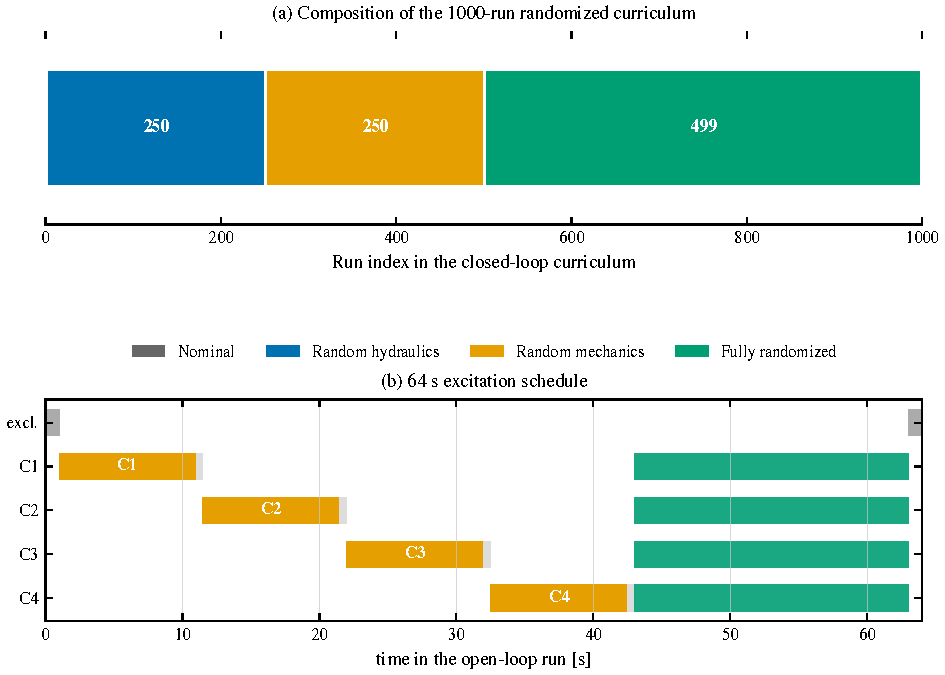
\includegraphics[width=\textwidth]{images/ch4/ch4_dataset_design}
  \caption{Design of the two collection campaigns.
  (a)~Composition of the closed-loop curriculum: one nominal run, then $250$
  hydraulics-only, $250$ mechanics-only and $499$ fully randomised draws.
  (b)~Timeline of one open-loop excitation run.}
  \label{fig:data:design}
\end{figure}

Two design choices carry into the deployment factors. Seal wear is one sampled
number driving three parameters together, so a worn cylinder becomes leakier and
slower at once: it scales piston clearance linearly, valve leakage area with the
cube of the same factor, and the spool time constant from $\unit[8]{ms}$ to
about $\unit[13]{ms}$ at the top of the range. Sampling the three independently
would have produced machines that are very leaky and yet perfectly fast. The
entrained-air and dead-volume coordinates randomise chamber dead volume over
$505$ to $\unit[579]{mL}$, which reaches the pressure dynamics through the
chamber volume in Equation~\eqref{eq:sys:continuity}, so compressibility enters
the batch as capacitance variation. The mechanical axes perturb all fourteen
rigid bodies: mass by up to $\pm 20\,\%$, centre of mass by up to $\pm 5\,\%$
of its nominal offset, and the inertia tensor consistently with the mass change,
so each body remains physically realisable. Joint stiffness and damping model
compliance in the bearings and linkage rather than in the fluid, and set how
much of a pressure transient appears as boom oscillation instead of clean
motion.

\section{Closed-Loop Data Collection}
\label{sec:data:closed-loop}

Algorithm~\ref{alg:data:closed-loop} in Appendix~\ref{app:data:curriculum}
gives the procedure that produced the curriculum above. The parameter table is
fixed before simulation and each run receives a new reference path.

\subsection{The Controller as a Data-Collection Instrument}

Every closed-loop run uses the same integral-backstepping controller at
$\unit[0.005]{s}$. Its gains remain fixed, so response differences are caused
by the plant draw rather than controller retuning.

Joint~2 uses PI control with velocity damping and gravity bias because it
carries the boom load. A barrier term enforces the URDF limits. Per-axis
command limits are $[0.95,\,0.95,\,0.80,\,0.80,\,0.90]$; the first four are
also stored in the inverse-dynamics checkpoint
(Section~\ref{sec:models:id}).

\section{Open-Loop Excitation Experiments}
\label{sec:data:open-loop}

\subsection{Limitations of the Closed-Loop Batch}

The first forward model achieved one-step $R^2\approx0.999$ on closed-loop
data but was almost insensitive to valve input: zeroing the input changed
long-horizon error by only a few percent
(Section~\ref{sec:models:fd-identifiability}). In closed loop, command is
largely determined by the state history already given to the model, so the
data do not separate command causality from state correlation
~\cite{ljung1999system}.

Figure~\ref{fig:data:regimes} confirms that coverage alone is not the issue.
The valve is saturated for about one quarter of a pooled run, operates at
mid-authority for roughly half, and otherwise remains in low-command creep.
Despite this spread, command and cylinder velocity remain concentrated along a
narrow band. The data are diverse in control effort but not identifiable,
motivating a separate open-loop experiment.

\begin{figure}[tb]
  \centering
  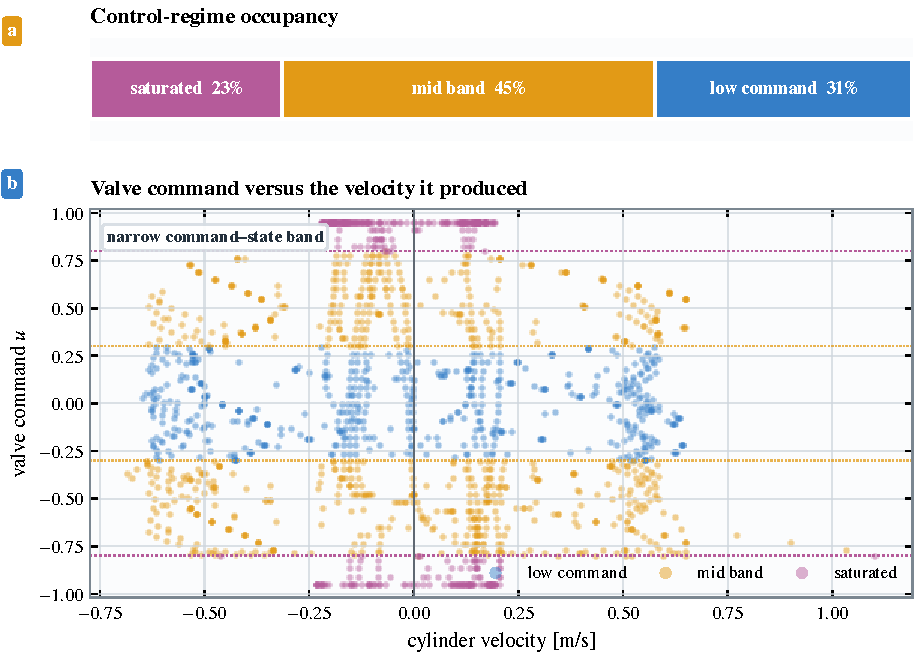
\includegraphics[width=\textwidth]{images/ch4/ch4_regimes}
  \caption{The closed-loop batch is diverse in control effort but
  not identifiable. (a)~Fraction of time the valve spends saturated, in the mid
  band and in low-command creep. (b)~The same run in the command--state plane,
  where the correlation that blocks identification is visible.}
  \label{fig:data:regimes}
\end{figure}

\subsection{Design of the Excitation Signal}

The excitation run lasts $\unit[64]{s}$ and follows the fixed schedule in
Figure~\ref{fig:data:design}(b). One second of startup is discarded, because
those samples describe the initialisation rather than the dynamics. Four
sequential slots follow, each giving one cylinder ten seconds of excitation
followed by a half-second zero-command gap that makes the segment boundaries
unambiguous. A twenty-second phase then drives all four channels at once, and a
final second of zero command closes the run. Commands are limited to $\pm 0.90$
of full authority.

An initial rapidly switching signal met the formal persistence condition but
kept each piston near one stroke position. The final design instead uses long
full-authority plateaus in the sequential phase and slow, high-authority motion
in the simultaneous phase. A slow near-square cycle is combined with distinct
medium-frequency channel components, with raised-cosine entry and exit ramps.
This provides both input excitation and useful stroke coverage.

\subsection{Plant Draws and Acceptance}

The same excitation is applied to four plant draws from the parameter space of
the closed-loop campaign: nominal, randomised hydraulics, randomised mechanics
and fully randomised. Holding the input fixed and varying only the plant makes
the four runs directly comparable.

Each run is checked for stroke coverage before acceptance, the collector
requiring at least $10\,\%$ of available stroke on cylinders 1--3 and $8\,\%$ on
cylinder 4. The retained runs cover $33\,\%$ of the stroke on cylinder 1 and
$12\,\%$ on cylinder 4, the narrowest of the four. Every channel clears the
floor, and Section~\ref{sec:data:diagnostics} confirms the material is
informative at these coverages.

The acceptance checks in Section~\ref{sec:data:diagnostics} verify that every
export contains independent state trajectories.

\section{Combining Closed-Loop and Open-Loop Datasets}
\label{sec:data:combining}

The inverse model uses only closed-loop data because its target is the
controller command for a measured state. The forward model is retrained on the
strict open-loop export while retaining closed-loop replay at weight $0.25$.
Without replay, four excitation runs do not provide enough pose coverage.

Figure~\ref{fig:data:coverage} shows the difference: closed-loop data covers
the reachable range, while open-loop data concentrates at identifiable valve
plateaus. The forward model therefore uses both.

\begin{figure}[tb]
  \centering
  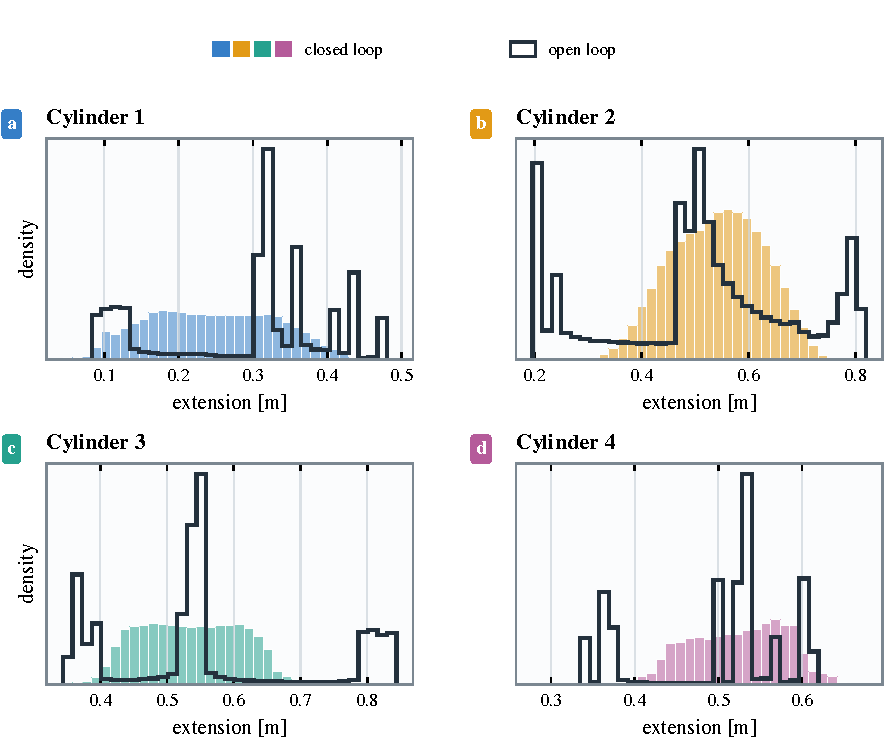
\includegraphics[width=\textwidth]{images/ch4/ch4_coverage}
  \caption{Extension coverage of the two campaigns, per cylinder
  and pooled over runs (closed-loop filled, open-loop outline). The closed-loop
  data fills the reachable range smoothly; the open-loop data concentrates into
  the plateaus where the valve is identifiable.}
  \label{fig:data:coverage}
\end{figure}

For ROM training, the inverse and forward exports are joined by run identifier,
time index and sample time. The join is accepted only when their
sixteen-dimensional cylinder states match sample for sample. It contains
$452\,400$ transitions at $\unit[0.05]{s}$ from $1\,040$ runs, split into
$936$/$52$/$52$ complete runs. Valve command is used only to supervise the
ROM's internal valve head; it is not a runtime input
(Section~\ref{sec:models:rom}).

This aligned nominal-plant export trains the inverse, forward and ROM models and
ships with the project, so every model-level result can be recomputed from the
file that produced it. Exact alignment, increment consistency and the
identifiability failure were checked directly on that export.


\section{Closed-Loop Calibration Data for the Command ROM}
\label{sec:data:rom-calibration}

The ROM drives a PhysX articulation whose compliance and contact response are
not present in Simscape. Further Simscape training cannot remove the resulting
deployment offset.

The calibration set therefore comes from closed-loop ROM--PhysX operation on
the native $\unit[0.05]{s}$ grid. Its $4\,084$ transitions store the six-step
runtime history and measured PhysX transition.

Only the command-gated correction head is trainable; all other parameters are
frozen and the correction is capped at $\unit[3]{mm}$. Original-data replay at
weight $0.25$ preserves wider pose coverage. The gate makes the correction
zero at zero command, retaining stationary hold.

The trajectories predate the moving-verge benchmark and exclude
cutter--ground contact. The bounded head limits, but does not remove, this
coverage gap. Section~\ref{sec:sys:rom-is-plant} explains the consequence for
the three-way comparison.

\section{The IsaacLab Deployment Collections}
\label{sec:data:isaaclab}

Two collections are recorded in the deployment plant. They share their factor
design, their domains, their splits and their freezing procedure, and differ in
one respect only: how the arm is driven. The first is driven by the task
controller and is the collection the inverse and forward models are scored
against in Section~\ref{sec:models:id-trust}; the second is driven by open-loop
excitation and is the one the adaptation module is trained on. Why both exist is
itself a result, and it is given in
Section~\ref{sec:data:openloop-collection}.

\subsection{Provenance of the Deployment Data}

The models that carry the identifiability argument, namely the system-dynamics
surrogate, the privileged factor encoder and the offline history encoder,
describe the plant the adaptive controller is closed around. That plant is the
command ROM plus PhysX, not the Simscape model. A surrogate identified on
Simscape data would be a model of a model, and the latent it defines would
describe variation the deployment plant does not necessarily exhibit. Both
collections are therefore made \emph{in} the deployment plant, and the frozen
ROM, ID and FD checkpoints enter this chain only as fixed components.

\subsection{The Physical Factor Vector}
\label{sec:data:factors}

The randomised quantity is a six-dimensional physical factor vector
%
\begin{equation}
  \label{eq:data:factorvec}
  \factorvec = \bigl[
    e_{\mathrm{flow}},\;
    e_{\mathrm{compliance}},\;
    e_{\mathrm{seal}},\;
    e_{\mathrm{pressure}},\;
    e_{\mathrm{mass}},\;
    e_{\mathrm{COM}_z}
  \bigr],
\end{equation}
%
with the ranges of Table~\ref{tab:data:factors}. Four coordinates are hydraulic
and two mechanical, which is what makes the hydraulic-only, mechanical-only and
combined domains of Section~\ref{sec:data:domains} separable. Each candidate was
admitted only after a one-factor sensitivity screen confirmed that moving it
alone produces a measurable change in cylinder extension, velocity, pressure or
end-effector motion.

One omission is deliberate. Actuation delay is not a randomised coordinate,
because delay here is an \emph{emergent} property of flow, compliance and load
rather than a free parameter. It is measured as a response property of each run
(Chapter~\ref{chap:evaluation}) rather than supplied to any model as a known
factor: handing an estimator a factor the real machine would never publish is
the same mistake as handing it the true payload.

\subsection{Domains and Factor Design}
\label{sec:data:domains}

Runs are organised into five domains
(nominal, hydraulic-only, mechanical-only, combined-training, and an
\emph{unseen} combined-test domain), and one factor vector is fixed for a complete run, so that no
run mixes plants. Factor configurations are drawn with deterministic
scrambled Sobol sequences~\cite{sobol1967distribution} rather than
independent uniform sampling, with explicit boundary anchors so that the
corners of the space are represented and not merely approached, and with
fixed per-domain seeds so the design is reproducible independently of
the data it produced. Combined draws that compound into an excessive
response gain are rejected at draw time rather than being collected and
discarded later.

The resulting design is auditable: $98.3\,\%$ of the factor keys are
unique, the active-factor matrix is full rank, every factor quartile is
populated, and the factor keys of the training, validation, and test
splits are disjoint. That last property is the one that matters most for
the claims of Chapter~\ref{chap:evaluation}: a test run does not merely
come from a different episode, it comes from a plant the models have
never seen.

\subsection{Collection Procedure: The Task-Controller Runs}

Every run is collected through the same interface the policy uses. The DLS
controller closes the loop on measured cylinder state and issues its command
through the four-dimensional action port into the command ROM and PhysX. No
joint-target bypass is used and no PPO policy collects identification data,
because a policy trained on the same plant would reintroduce the closed-loop
correlation that Section~\ref{sec:data:open-loop} spent a campaign removing.

Independent excitation is supplied by dedicated four-channel PRBS windows
through that same action port, at small amplitude and a hold of ten control
steps, so the excitation is causally independent of the state without leaving
the safe envelope. Probe actions are logged separately from controller output.
Each run follows a fixed eleven-segment structure (settle, three postures, three
PRBS windows, DLS task motion, reach-and-return and stow). As recorded, each
run is $11\,520$ control steps and $\unit[192.0]{s}$ of simulated time.

Figure~\ref{fig:data:isaaclab-collection} summarises the IsaacLab collection
configuration and its frozen run-level outputs.

\clearpage
\begin{figure}[H]
  \centering
  \begin{tikzpicture}[x=1cm,y=1cm,font=\normalsize,
    card/.style={draw=black!55,line width=.8pt,rounded corners=2pt,
      fill=white,minimum height=2.05cm,align=center,inner sep=6pt}]

    \node[font=\Large\bfseries,text=black!85] at (0,.42)
      {ISAACLAB ADAPTATION COLLECTION};

    \node[draw=black!45,line width=.8pt,inner sep=3pt]
      (plant) at (0,-4.25)
      {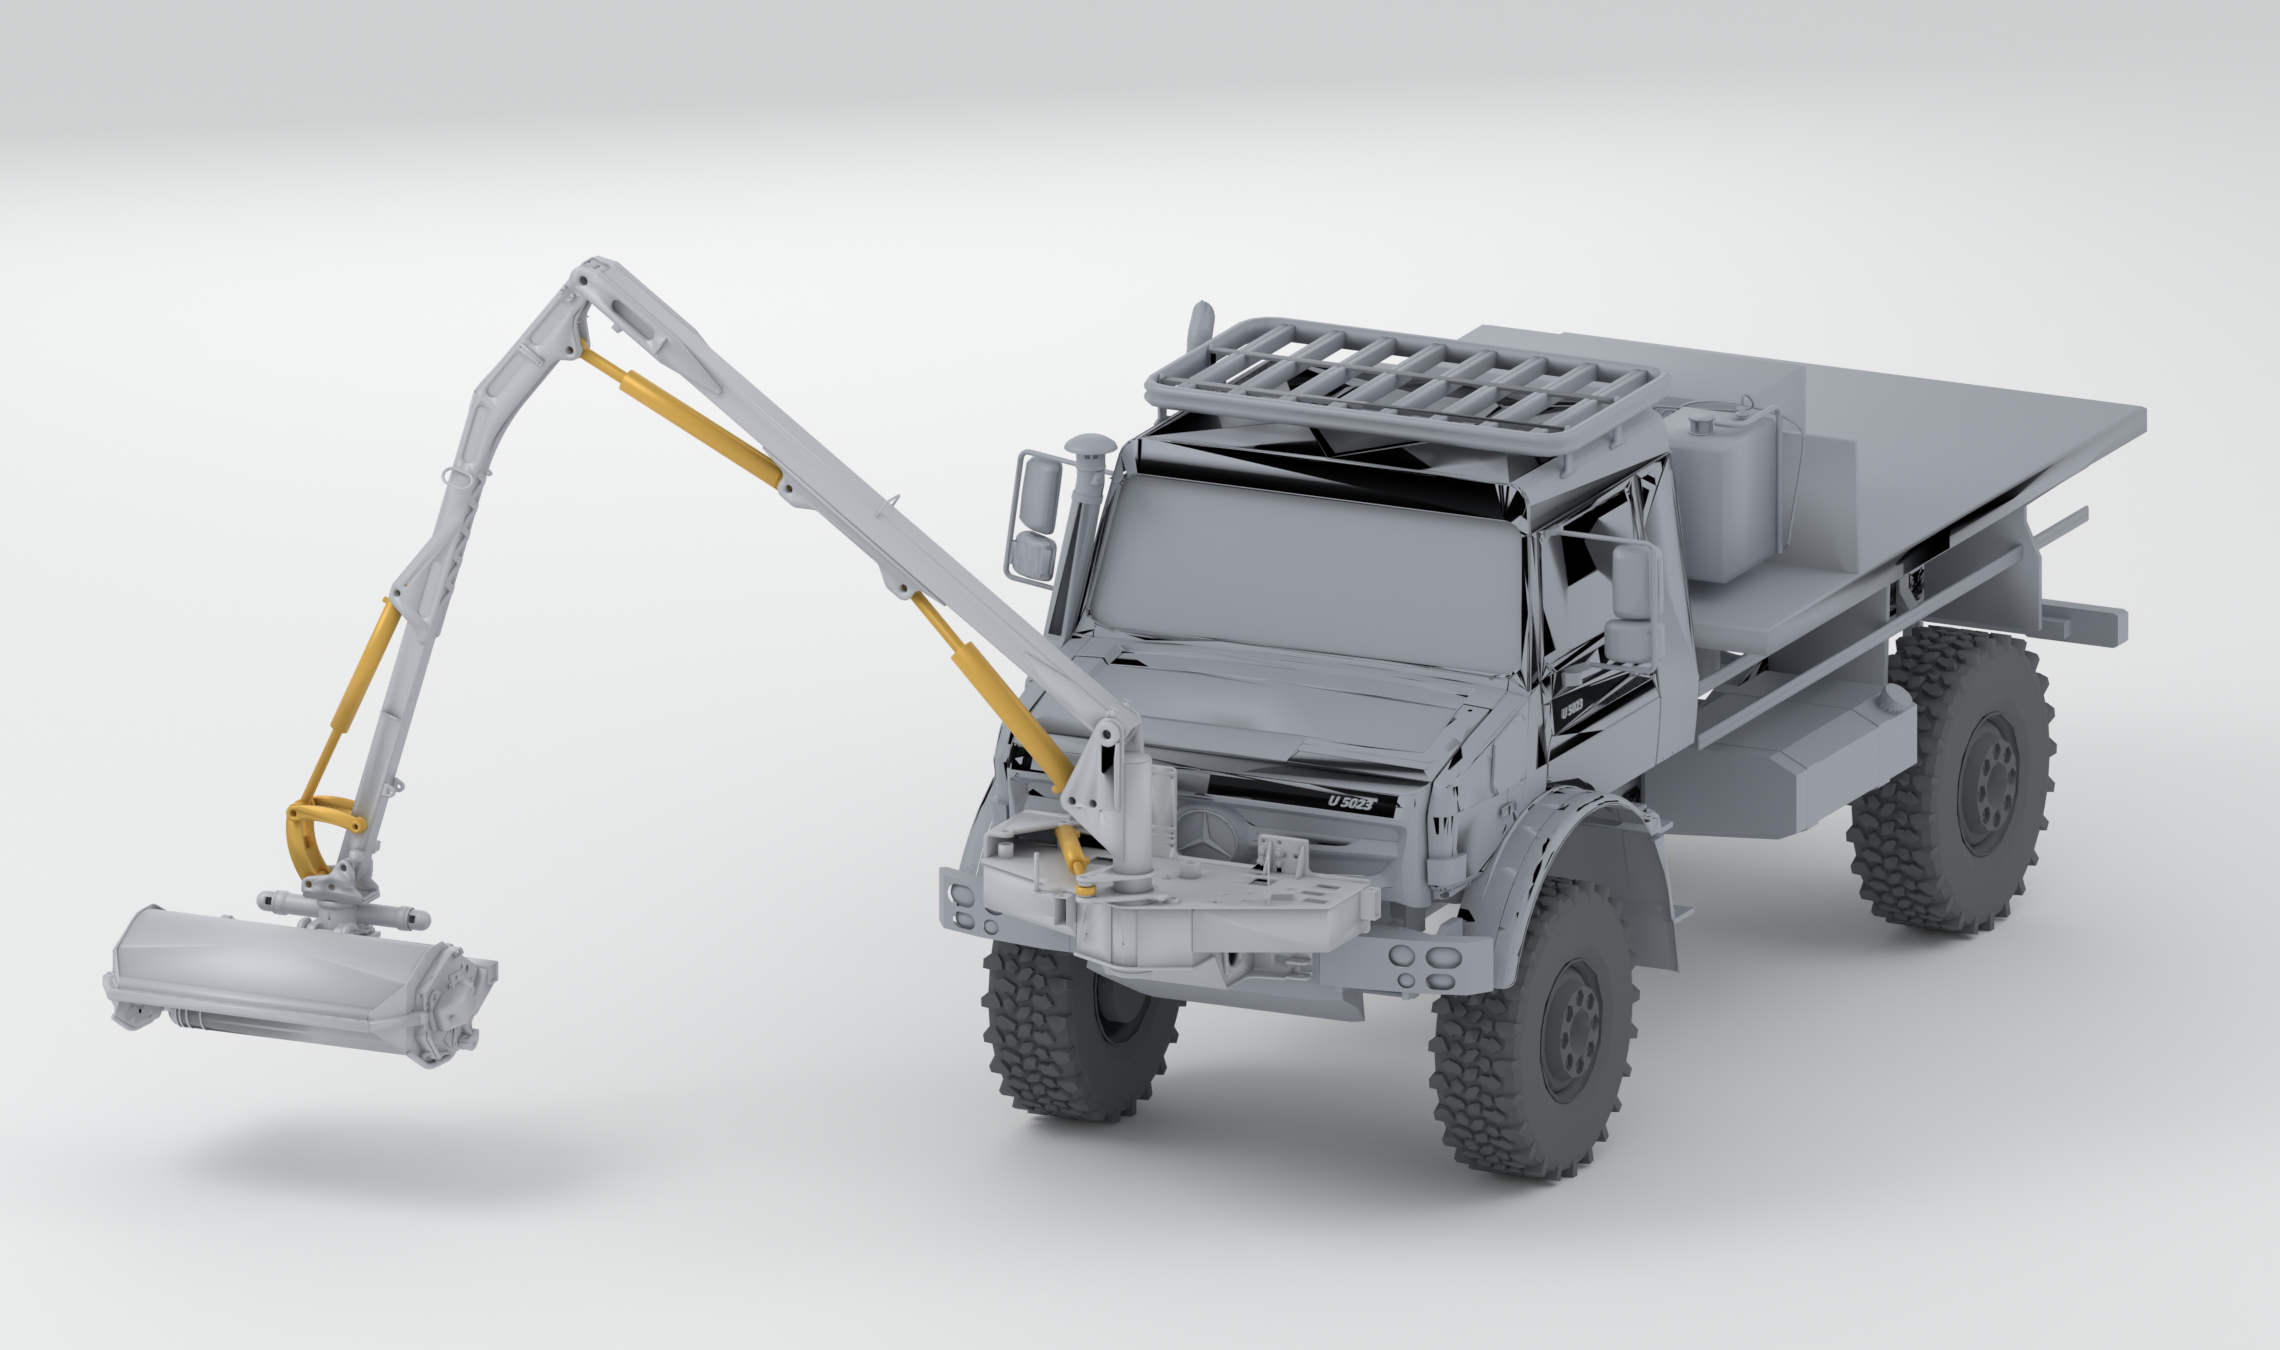
\includegraphics[width=13.35cm]{images/ch4/unimog_mulag_iso_v2.png}};

    \draw[black!35] (-6.75,-8.82) -- (6.75,-8.82);

    \node[card,text width=3.75cm] at (-4.55,-10.20)
      {\textbf{PLANT DRAWS}\\[6pt]
       \small four hydraulic\\two mechanical};
    \node[card,text width=3.75cm] at (0,-10.20)
      {\textbf{EXCITATION}\\[6pt]
       \small DLS motion\\PRBS probes};
    \node[card,text width=3.75cm] at (4.55,-10.20)
      {\textbf{RUN RECORD}\\[6pt]
       \small state $\bullet$ action\\factor key};

    \node[font=\large\bfseries,text=black!85] at (0,-12.75)
      {FROZEN DATASET};
    \node[font=\small,text=black!60] at (0,-13.55)
      {$118$ accepted runs $\bullet$ disjoint run-level splits};

    \node[card,text width=3.15cm,minimum height=1.40cm]
      at (-4.15,-15.15) {\textbf{TRAIN}\\[3pt]$82$ runs};
    \node[card,text width=3.15cm,minimum height=1.40cm]
      at (0,-15.15) {\textbf{VALIDATION}\\[3pt]$20$ runs};
    \node[card,text width=3.15cm,minimum height=1.40cm]
      at (4.15,-15.15) {\textbf{HELD-OUT TEST}\\[3pt]$16$ runs};
  \end{tikzpicture}
  \caption{IsaacLab adaptation-data collection. Each run uses one fixed
  six-factor plant draw and combines DLS task motion with independent PRBS
  probes. State, action and factor keys are logged, audited and frozen into
  disjoint train, validation and held-out test splits.}
  \label{fig:data:isaaclab-collection}
\end{figure}
\clearpage

\subsection{The Open-Loop Context-Identification Collection}
\label{sec:data:openloop-collection}

A second collection of $118$ runs was recorded in the same deployment plant,
with the same six-factor design and the same domain and split structure, and it
is the offline context-identification collection used to train the AAM. It
differs from the collection
above in a single respect, and that respect is the point of it: there is no task
controller. Each run is driven by open-loop excitation alone, the vehicle is
stationary, and no policy is in the loop. The excitation is the same
four-channel PRBS used as a probe above, at amplitude $0.02$ and held for ten
control steps, but it now drives the whole run rather than three windows inside
one. Each run is $11\,040$ control steps, giving $1\,302\,720$ steps across the
collection.

The reason for collecting twice is structural. Under a task controller the
command is computed from the state, so command and response are close to
redundant and a plant descriptor has little left to explain; a model asked to
identify the plant from that data is being given a question with no answer in
it, and what it reports is a property of the data rather than of the
architecture. Removing the controller makes the question well posed, which is
why every model-level result in this thesis is fitted on this collection. How
rich the excitation must be, and the amplitude beyond which plant identity stops
being recoverable, remain outstanding measurements.

What each consumer takes from the recorded feature contract is set out in
Section~\ref{sec:data:history-features} for the adaptation module and
Section~\ref{sec:data:sd-features} for the prediction models.

\subsection{The Frozen Dataset}

Both collections contain $118$ complete runs under the identical domain design:
$2$ nominal, $40$ hydraulic-only, $12$ mechanical-only, $48$ combined-training
and $16$ unseen combined-test. Collection ran in four vectorized IsaacLab
environments with per-environment factors and logging, and slots that tripped a
safety or validity check were discarded and retried individually. All $118$ runs
passed the final collection gate, which checks finite physics, exact model-grid
alignment, command rank, factor-response authority, state coverage and
saturation limits.

Each dataset is then \emph{frozen}: the raw runs are checksummed and the
run-level split is fixed at $82$ training, $20$ validation and $16$ reserved
combined-test runs, with zero factor-key leakage between them. The reserved
sixteen do not influence history length, checkpoint, hyperparameter or
architecture selection; they are scored only after each model is fixed, and test
results are reported with validation results rather than in place of them.

\subsection{Learning Timebase and Hydraulic State}

The learning timebase is the actuator model grid, not the control clock.
Samples are exact $\unit[50]{ms}$ ROM transitions taken at control
indices $0, 3, 6, \dots$: state row $t$ and command row $t$ predict
state row $t+3$. Nothing is interpolated. This is the same alignment
rule as Section~\ref{sec:sys:timing}, and it is enforced rather than
assumed, because a model trained across a mismatched interval is wrong by a fixed factor in the quantity it exists to supply.

The hydraulic state used by the system-dynamics surrogates is
%
\begin{equation}
  \label{eq:data:sdstate}
  \bm{s}_t = \bigl[\bm{x}_t^{1:4},\; \dot{\bm{x}}_t^{1:4},\;
  \Delta\bm{p}_t^{1:4}\bigr] \in \mathbb{R}^{12},
\end{equation}
%
with joint position and velocity carried as \emph{context} only, and the
prediction target the next $\unit[50]{ms}$ state delta. Differential pressure
is not a measured signal. At runtime it is the actuator model's recursive
state, generated by the command ROM or frozen forward model
(Section~\ref{sec:sys:actuation}). The system-dynamics surrogate and AAM may use it
because it exists inside the deployed loop, but it inherits actuator-model
error. Causal history is therefore retained to represent pressure transients
that one sample cannot summarise.

\section{Feature and Target Construction}
\label{sec:data:features}

\subsection{The Actuator Models}

The three learned actuator models take cylinder-space features, in the
ordering and notation fixed in Section~\ref{sec:models:overview}. Their
input contracts differ because their questions differ. The inverse model
receives the measured cylinder state, the logged rod forces, the desired
increments, and the previously applied command, twenty-eight numbers in
all. The forward model receives the applied valve command and the
measured state, twenty numbers. The reduced-order model receives a
six-sample history of state, previously predicted valve, and desired
command, twenty-four numbers per step.

Three conventions apply throughout, and they are the same ones the models
enforce at inference time.

\paragraph{Increment Targets}
Every dynamic target is a within-run one-step increment,
$\Delta \bm{x}_k = \bm{x}_{k+1} - \bm{x}_k$, never an absolute state. This
removes the large static component of the signals and turns the trivial
persistence solution into an explicit baseline rather than a hiding place.

\paragraph{Causal Alignment}
Features at step $k$ contain only quantities available at step $k$. The
extraction stage verifies this by recomputing every logged target from
the within-run difference of the states and requiring exact agreement,
a check reported in Section~\ref{sec:data:diagnostics}.

\paragraph{Time-Base Conversion}
The open-loop campaign is logged at $\unit[0.01]{s}$ but the models run at
$\unit[0.05]{s}$, so five consecutive raw samples are combined into one
transition. The valve input attributed to that transition is the command held at
the start of the window, which is the causally correct choice; the window mean is
recorded for analysis only. Cylinder extension velocity is not logged directly
in the closed-loop archive and is obtained by differentiating extension on the
output grid, consistent with the trapezoidal identity that the strict data
satisfies to $R^2 = 0.994$--$0.9997$ (Equation~\ref{eq:models:trapezoid}).

\subsection{Features and Targets for the Adaptation Module}
\label{sec:data:history-features}

The adaptation module is trained on the open-loop collection of
Section~\ref{sec:data:openloop-collection}. Its history window carries only
quantities the deployed stack produces at runtime: the five joint positions, the
five joint velocities, the four cylinder pressure differences and the four
previously applied valve commands, giving the eighteen-value row of
Section~\ref{sec:models:aam}. The pressure entry is the learned actuator's own
recursive state rather than a measurement
(Section~\ref{sec:sys:actuation}, Table~\ref{tab:sys:signals}); it is admitted
because the model that generates it runs inside the deployed loop, and the
consequence of that choice is examined where the estimator is evaluated. Four
classes of signal are excluded by construction, and the exclusion is enforced by
an explicit input mask rather than by convention:

\begin{itemize}
  \item the physical factors $\factorvec$ and the true latent $\latent$,
    because recovering them is the estimator's job;
  \item any future observation, because the estimator is causal;
  \item the hidden internal state of the command ROM, because the
    deployment interface does not expose it;
  \item the desired task reference, so that the latent describes the
    plant rather than the trajectory being asked of it.
\end{itemize}

Windows are contained within a single run, and each carries the
stopped-gradient target $\latent = \mu(\factorvec)$ of its own run together with
the run identifier, domain, split and valid history bounds. Applied to the $118$
frozen runs this yields $434\,240$ rows, of which $431\,998$ carry a complete
twenty-step window ($3\,661$ per run; the first nineteen ticks of a run cannot
fill one). What is built from them belongs to Chapter~\ref{chap:models}.

The residual encoder deployed in \ppoAAMFD{} uses no collection at all, for the
reason given in Section~\ref{sec:data:onpolicy}, and it does not read this row.
It reads the whole $66$-value policy observation together with the four
previously applied valve commands, $70$ values per step. The row defined here is
the contract of the explicit estimator only. What the wider input costs is
examined in Section~\ref{sec:eval:adaptation}.

\subsection{Features and Targets for the Prediction Models}
\label{sec:data:sd-features}

The prediction models read the same runs through a third contract: a transition
at the $\unit[50]{ms}$ tick rather than a history window, and the privileged
factor vector $\factorvec$, which the adaptation module never sees and which is
what allows them to define the target the module is then asked to recover. That
contract is set out with the dataset it produces in
Section~\ref{sec:data:system-dynamics}, because what it is for is only visible
alongside the audit it makes possible.

\subsection{On-Policy AF Adaptation Rollouts}
\label{sec:data:onpolicy}

The context columns that carry the adaptation result in \ppoAAMFD{} are not
trained from the frozen collection above. They have no dataset and no run-level
splits, because they are optimised under the reinforcement objective, so their
training data is the on-policy experience the stack generates as it learns.

What replaces the dataset is a plant design, since on-policy training makes the
training distribution a property of the environment rather than of a file. The
cutter mass is resampled per episode across a range spanning one to five times
nominal. One fixed compromise is then unlikely to suit the whole family, which
is what gives a controller something to gain from knowing which member it is
driving, without assuming in advance that it will.

The estimator that supplies that knowledge at deployment does have a dataset,
and it is collected after policy training rather than before: a mixed-payload
rollout of the trained policy, with the $66$ task channels regressed onto the
payload that produced them. It is refitted for each training seed, because the
regression is on the observation distribution that policy induces and a
different policy induces a different one. Whether the correct payload
contributes beyond conditioning on any plausible one is tested against a
permuted-payload control in Section~\ref{sec:eval:adaptation}.

One property of the frozen collection is inherited unchanged: the plant is still
the deployment plant, so the change of training regime does not substitute a
different system. The history row is not inherited. The residual encoder reads
the full policy observation and the previous valve command rather than the
eighteen-value row, so the exclusion contract above does not apply to it. That
is stated where the residual is defined
(Section~\ref{sec:ctrl:af-residual}) and carried into
Section~\ref{sec:eval:adaptation}, where it becomes the leading candidate
explanation for what the adaptation experiment finds.

\section{Preprocessing and Data Splits}
\label{sec:data:preprocessing}

Splitting is done at the level of complete runs, never of individual samples,
because a random sample-level split would place transitions from the same
trajectory on both sides of the boundary and report a score that mostly measures
interpolation within a run. For the command-conditioned dataset the $1\,040$
runs are divided into $936$ training, $52$ validation and $52$ test runs, giving
$407\,160$, $22\,620$ and $22\,620$ transitions, with no run identifier in more
than one split. The IsaacLab deployment collection is split by run \emph{and} by
factor configuration ($82$/$20$/$16$), the stronger condition: separating runs
alone would let two runs of the same plant fall on opposite sides of the
boundary and turn a claim about unseen plants into a claim about unseen
episodes.

The strict open-loop export needs different treatment because it contains only
four runs, and holding one out would remove an entire plant draw from training.
Each run is instead divided into twenty temporal blocks, every fifth block is
assigned to validation, and a five-sample guard interval is discarded at each
boundary so that no $\unit[0.05]{s}$ transition window spans the split. This
preserves comparable target distributions in training and validation.

Normalisation statistics are computed on the training split only and stored
inside each checkpoint, so a model always normalises with the statistics it was
fitted with; the loader enforces the stored contract rather than recomputing it.
Samples are carried with an explicit validity flag rather than silently dropped,
$93.7\,\%$ of the strict export being marked valid and the remainder being the
excluded startup and shutdown seconds and the zero-command gaps. Keeping them
with a flag means the time base stays contiguous and the within-run difference
checks remain meaningful.

\section{Dataset Diagnostics}
\label{sec:data:diagnostics}

No dataset in this thesis is used before it passes an explicit audit,
for the reason given at the end of
Section~\ref{sec:data:open-loop}. The audit of the strict open-loop
export is reproduced in Table~\ref{tab:data:audit}.



The two rank figures speak directly to requirement R2. The instantaneous command
matrix has rank four, so no channel is a linear combination of the others, and
the lagged regressor matrix built from the command history has rank eighty, so
the excitation is persistently exciting to the order the models need. The
condition number of that lagged matrix is about $4.6\times10^{3}$, finite and
workable rather than comfortable, and it is the price paid for the stroke
coverage the long plateaus buy.

The three increment checks return a maximum error of exactly zero, which is
expected rather than suspicious: the targets are computed from the logged states
by the same within-run difference the check recomputes, so the check verifies
that the extraction stage did what it claims rather than that the simulation is
accurate. It catches misalignment, off-by-one indexing and rows reordered or
concatenated across run boundaries. Physical fidelity is addressed separately by
the validation study of Section~\ref{sec:sys:simscape-validation}.

Two properties of the Simscape material are recorded here because later chapters
refer to them. Stroke coverage is $12\,\%$ on the head-pivot cylinder, the
narrowest of the four channels and also the one the strict forward model
predicts least well. The rod-force channel carries zero supervised weight in the
reduced-order model, a design choice rather than a data defect: force is
generated internally by the PhysX plant at deployment, and the logged channel
additionally fails a piston-area consistency check on this export. No result
rests on it.

The IsaacLab collection is audited against different failure modes: design
adequacy before use (unique factor keys, full active-factor rank, disjoint keys
across splits), physical validity per run (finite physics, exact model-grid
alignment, full command rank, bounded saturation), and leakage structurally,
with privileged channels removed by an explicit input mask rather than by
trusting the feature list. Its limitation is scale, $118$ runs over six factors
being a sparse design, which is why the paired test of
Section~\ref{sec:data:sd-audit} is reported with bootstrap intervals and per-run
detail rather than as a pooled point estimate. That limitation does not bound
the closed-loop adaptation result, which is estimated from paired environments
generated on-policy under the plant design of
Section~\ref{sec:data:onpolicy}.

\section{The System-Dynamics Dataset}
\label{sec:data:system-dynamics}

The prediction models read the deployment collection through a third contract,
built once and frozen with the rest. It is a derived view rather than a separate
collection: the same $118$ runs, resampled from the $\unit[60]{Hz}$ control log
to the $\unit[20]{Hz}$ model tick by taking every third step, giving $3\,840$
transitions per run and $453\,120$ in total. The run-level split is inherited
unchanged, $82$ training, $20$ validation and $16$ test runs, so a run
contributes to exactly one split here and in every other view of this data.

Each sample is one transition. The input is the $12$-dimensional hydraulic
state, the $10$-dimensional joint context and the valve command pair, previous
and current, for $30$ channels; the target is the hydraulic-state increment to
the next tick in the same $12$ dimensions. Training draws five consecutive
transitions at a time, so the objective is a short rollout rather than a
one-step fit. Four per-tick flags record cylinder limit, command saturation,
valve saturation and non-finite physics, so a model can be scored on valid ticks
alone. Each run carries its own six-factor vector $\factorvec$, which is
privileged: it is what allows a target to be defined for the adaptation module
of Section~\ref{sec:data:history-features}, and it is masked out of every
deployable input.

\subsection{Dataset Separation Across Plants}
\label{sec:data:sd-audit}

One property of this dataset cannot be checked by an audit of its structure. The
checks of Section~\ref{sec:data:diagnostics} establish that the runs are valid,
that the factor design is full rank and that the splits do not leak, but not
that the runs \emph{differ by plant} in a way any model could use. If they do
not, nothing built on this dataset can recover the difference.

The test is a paired one on the dataset itself. Two prediction models are
trained on identical samples, splits and objective; one receives a
two-dimensional plant context from an encoder $\latent = \mu(\factorvec)$
trained jointly with it, and the matched control receives no such input. Neither
is an actuator and neither enters a control stack.

The context helps, and narrowly. Pooled rollout error falls by
$7.20\times10^{5}$ on the $20$ validation runs, with a $95\,\%$ interval of
$[-1.03\times10^{6},\, -4.30\times10^{5}]$, and by $4.41\times10^{5}$ on the
$16$ test runs, interval $[-7.61\times10^{5},\, -1.74\times10^{5}]$. Both
exclude zero, so the dataset does separate plants. Where it separates them is
the more useful result: the per-channel decomposition puts the whole gain in
pressure, and the extension and velocity intervals cross zero on both pools.

\begin{table}[H]
  \centering
  \caption{Per-channel decomposition of the paired advantage at a $20$-tick
  horizon, pooled over $36$ held-out runs. Values are the mean paired difference
  between the context-conditioned model and the matched control, with a
  $95\,\%$ bootstrap interval. The advantage is confined to pressure.}
  \label{tab:data:latent-channels}
  \begin{tabular}{lccc}
    \toprule
    Channel & mean paired difference & $95\,\%$ interval & excludes zero \\
    \midrule
    extension & $5.2\times10^{-5}$ & $[-3.6\times10^{-5},\; 1.4\times10^{-4}]$ & no \\
    velocity  & $-2.4\times10^{-4}$ & $[-7.1\times10^{-4},\; 2.4\times10^{-4}]$ & no \\
    pressure  & $1.75\times10^{5}$ & $[2.1\times10^{4},\; 3.3\times10^{5}]$ & yes \\
    \bottomrule
  \end{tabular}
\end{table}

Two limits travel with this result and both matter later. It compares separately
trained models, so it establishes that the context is informative, not that an
estimator could recover it or that a controller could use it;
Section~\ref{sec:models:chain} substitutes contexts within one model, which is
the tighter test. And the informative channel is pressure, which the controller
does not integrate. That is the first appearance of the delivery problem the
rest of this thesis runs into: this dataset carries plant identity in the one
channel that reaches the command path least directly.

With the data described and audited, the next chapter turns to what was
learned from it: the inverse and forward models that form the
\ppoIDFD{} actuator path, the command-conditioned reduced-order model that
replaces them in \ppoROM, and the adaptation module that estimates at runtime
what the surrogate above was given.

\RRLABchapterblank
%%%%%%%%%%%%%%%%%%%%%%%%%%%%%%%%%%%%%%%%%%%%%%%%%%%%%%%%%%%%
%% Chapter 5 — Learned Models and Online Adaptation
%% Target length: 14 pages.
%% Purpose: develop the learned actuator representations, their
%% training objectives, and the adaptation chain; separate what the
%% evidence establishes and the scope of each result.
%% Deployment-level gate results belong to Chapter 7 and are not
%% repeated here.
%%%%%%%%%%%%%%%%%%%%%%%%%%%%%%%%%%%%%%%%%%%%%%%%%%%%%%%%%%%%
\chapter{Learned Models and Online Adaptation}
\label{chap:models}

Chapter~\ref{chap:data} established how the datasets were generated and why
both closed-loop operation and open-loop valve excitation were required. This
chapter develops the learned representations that consume them: the
inverse-dynamics (ID) and forward-dynamics (FD) networks of the \ppoIDFD{}
actuator path, the command-conditioned reduced-order model (ROM) that replaces
them in \ppoROM, and the system-dynamics surrogate, privileged factor encoder
and Arm Adaptation Module (AAM) that together carry the adaptation argument.

Two commitments organise the chapter. The first is that the surrogate is kept
strictly separate from the deployed actuator: the system-dynamics model is an
instrument for establishing whether a compact dynamics latent exists and is
useful, never a component of any control stack. The second is that no model is
accepted on a supervised score, because a recurring result of this work is that
such scores can be not merely optimistic but uninformative: a forward model
reached a one-step $R^2$ near $0.999$ while having learned almost nothing about
valve authority (Section~\ref{sec:models:fd}). Every model is therefore
presented with its contract, training objective, and the offline evidence that
accepted or refused it. All models operate on cylinder-space signals; the
mapping to task space belongs to Chapter~\ref{chap:system}, the control
integration to Chapter~\ref{chap:control}, and deployment-level results to
Chapter~\ref{chap:evaluation}.

\section{Modelling Overview and Common Notation}
\label{sec:models:overview}

All learned models act on the four hydraulic cylinders of the MULAG arm,
indexed $i \in \{1,\dots,4\}$ in the fixed order slew cylinder
(\emph{Drehzapfen}), boom cylinder~I (\emph{Ausleger~I}), boom cylinder~II
(\emph{Ausleger~II}) and head pivot cylinder (\emph{Messerkopf-Schwenk}). The
passive fifth joint is not actuated and enters no model input. At the
learned-model sample time $T = \unit[0.05]{s}$ the discrete index $k$ refers to
the cylinder extension $\bm{x}_k$, the extension velocity $\dot{\bm{x}}_k$, the
chamber pressure difference $\Delta\bm{p}_k$ and the logged rod force
$\bm{F}_k$, each in $\mathbb{R}^4$. The valve command
$\bm{u}_k \in [-1,1]^4$ is the normalised spool command of the four
proportional valves. The desired cylinder command produced by the task
controller is the pair
%
\begin{equation}
  \label{eq:models:command}
  \bm{c}_k = \bigl[\Delta\bm{x}^{*}_k,\; \Delta\dot{\bm{x}}^{*}_k\bigr]
  \in \mathbb{R}^{8},
\end{equation}
%
the extension and extension-velocity increments to be realised over the next
sample. Predictions carry a hat, and $\Delta(\cdot)_k = (\cdot)_{k+1} -
(\cdot)_k$ denotes a within-run one-step increment throughout.

\begin{figure}[tbp]
  \centering
  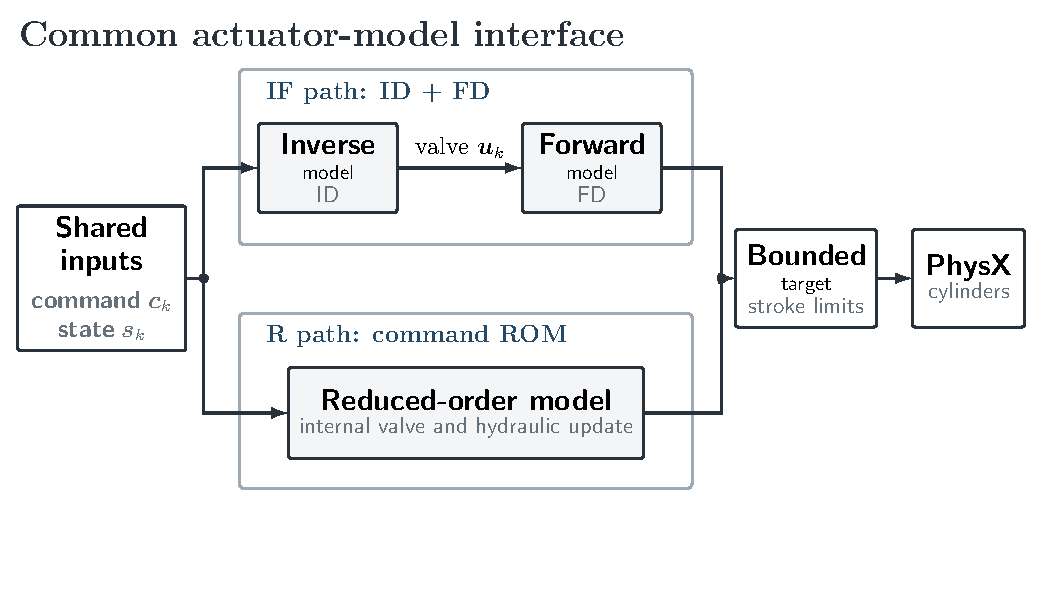
\includegraphics[width=\textwidth]{images/models_overview}
  \caption{Common interface of the two alternative actuator paths. Both
  receive the desired cylinder command and measured hydraulic state, and both
  produce the same bounded PhysX cylinder target. The \ppoIDFD{} path composes
  the inverse and forward models; the \ppoROM{} path uses one
  command-conditioned reduced-order model.}
  \label{fig:models:overview}
\end{figure}

Figure~\ref{fig:models:overview} compares the actuator paths. In \ppoIDFD, the
ID maps the state and desired increment to a valve command, and the FD predicts
the resulting increment. In \ppoROM, one command-conditioned model predicts
the valve internally and propagates pressure, velocity and extension. Both
paths produce the same bounded PhysX cylinder target in
IsaacLab~\cite{mittal2023orbit} under the same policy action
contract~\cite{schulman2017proximal}.

Three conventions apply throughout. Dynamic targets are within-run increments,
with $\Delta\hat{\bm{x}}=\bm{0}$ as the persistence baseline. Each checkpoint
uses its own training-set normalisation. Inputs at step $k$ are causal, and
targets are measured transitions to step $k+1$.

Simscape supplies the identification data described in Chapter~\ref{chap:data}.
The exported arrays are audited, frozen and used to train the models in
PyTorch~\cite{paszke2019pytorch}; Simscape is not part of training or
deployment.

The closed-loop Simscape export~\cite{mathworks2024simscape} contains
$452\,400$ transitions at $T=\unit[0.05]{s}$ from $1\,040$ runs, split by run
into $936/52/52$ training, validation and test runs. It supplies the supervised
ID, FD and command-ROM data. The FD repair uses four open-loop $64$-s runs at
$\unit[0.01]{s}$ with rank-4 valve excitation on four plant draws.

\section{Inverse Dynamics Model}
\label{sec:models:id}

The ID network maps the current hydraulic state and desired cylinder increment
to a valve-command change:
%
\begin{equation}
  \label{eq:models:id-contract}
  \Delta\bm{u}_k = f_{\mathrm{ID}}
  \bigl(\bm{x}_k,\, \dot{\bm{x}}_k,\, \Delta\bm{p}_k,\, \bm{F}_k,\,
        \Delta\bm{x}^{*}_k,\, \Delta\dot{\bm{x}}^{*}_k,\, \bm{u}_{k-1}\bigr)
  \in \mathbb{R}^4 ,
\end{equation}
%
a 28-dimensional input. The deployed command is
$\bm{u}_k = \operatorname{clip}(\bm{u}_{k-1} + \Delta\bm{u}_k,\,
-\bm{u}_{\max},\, \bm{u}_{\max})$ with per-axis limits
$\bm{u}_{\max} = [0.95,\, 0.95,\, 0.8,\, 0.8]$ stored in the checkpoint.
The change formulation retains the previous valve operating point near the
direction-dependent dead zone (Section~\ref{sec:fund:actuation-chain}). Logged
achieved transitions serve as desired increments because no independent
cylinder-space reference was recorded.

The 512-wide residual MLP~\cite{he2016deep} uses SiLU activations, layer
normalisation and dropout~\cite{elfwing2018sigmoid,ba2016layer,srivastava2014dropout}.
Adam minimises a smooth-$L_1$ loss on normalised targets, with saturated samples
up-weighted~\cite{kingma2015adam,huber1964robust}.

Figure~\ref{fig:models:id-architecture} separates the three input groups and
shows the four residual blocks explicitly. The network predicts a four-axis
valve-command increment, which is accumulated and clipped before use.

\begin{figure}[H]
  \centering
  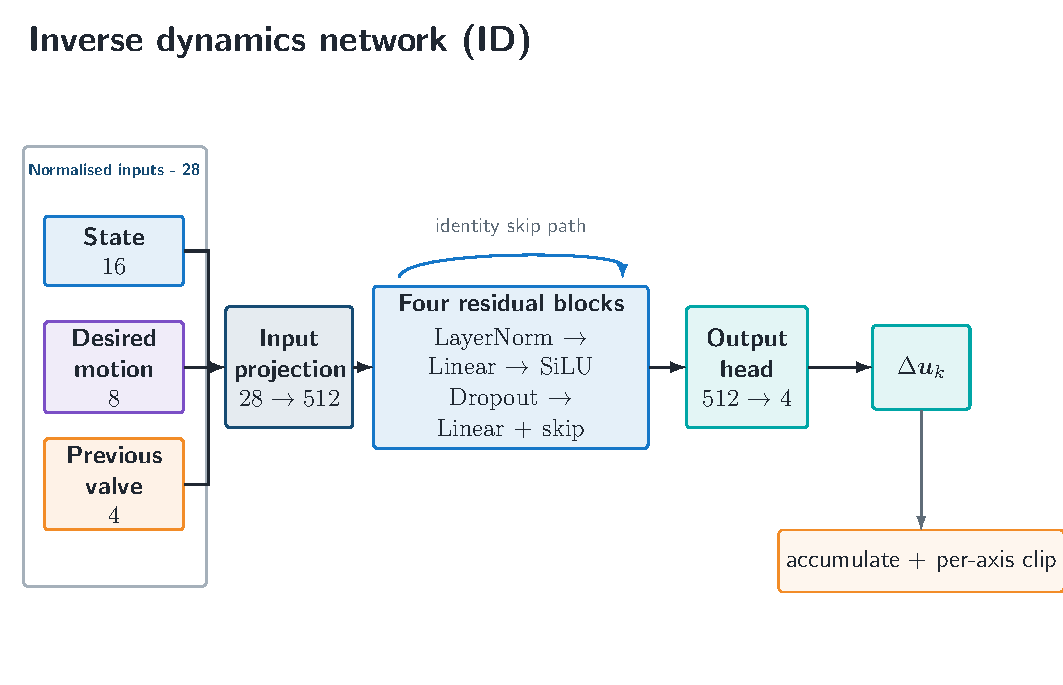
\includegraphics[page=1,width=\textwidth]{images/ch5_network_architectures}
  \caption{Inverse-model architecture. Current hydraulic state (16), desired
  motion (8) and the previous valve command (4) form the 28 inputs. A
  512-wide, four-block residual MLP predicts $\Delta\bm{u}_k$, which is
  accumulated and clipped per axis to form the bounded valve command.}
  \label{fig:models:id-architecture}
\end{figure}

Per-valve validation $R^2$ is $0.9973$--$0.9996$. This shows reproduction of
logged commands, not plant authority: in closed-loop data, achieved transitions
and logged commands are correlated (Section~\ref{sec:fund:identifiability}).

\subsection{Paired Control Fine-Tuning}
\label{sec:models:id-paired}

The composite is assessed by the \emph{paired differential response}: the FD
prediction under the ID command for the requested target minus the prediction
under its command for a zero target,
%
\begin{align}
  \bm{u}^{\mathrm{tgt}}_k &= f_{\mathrm{ID}}(\cdot,\, \bm{c}_k,\, \bm{u}_{k-1}),
  \qquad
  \bm{u}^{0}_k = f_{\mathrm{ID}}(\cdot,\, \bm{0},\, \bm{u}_{k-1}), \notag \\
  \Delta\hat{\bm{x}}^{\mathrm{pair}}_k &=
    f_{\mathrm{FD}}\bigl(\bm{u}^{\mathrm{tgt}}_k, \cdot\bigr)
  - f_{\mathrm{FD}}\bigl(\bm{u}^{0}_k, \cdot\bigr).
  \label{eq:models:paired}
\end{align}
%
Before fine-tuning, the composite normalised control error was $1.00$, equal to
the zero-response baseline, and all regression slopes were below $0.004$
(Table~\ref{tab:models:paired}). The networks were fine-tuned jointly on
$\mathcal{L}_{\mathrm{ctl}} = \| \Delta\hat{\bm{x}}^{\mathrm{pair}}
- \Delta\bm{x}^{*} \|^2_{\mathrm{norm}}
+ \lambda_{\mathrm{ID}}\mathcal{L}_{\mathrm{ID}}
+ \lambda_{\mathrm{FD}}\mathcal{L}_{\mathrm{FD}}$,
with the supervised terms retained. Target blocks were shuffled across valid
states to break the logged state--target pairing. After 30 epochs, control
error fell to $0.109$; all slopes exceeded $0.8$ and all correlations exceeded
$0.92$. This frozen checkpoint is used in \ppoIDFD{} and \ppoAAMIDFD{}.

\begin{table}[H]
  \centering
  \caption{Effect of paired control fine-tuning on the composite differential
  response \eqref{eq:models:paired}, per cylinder axis on validation data.
  Before fine-tuning the composite had essentially no control authority despite
  near-perfect supervised scores of both networks; the composite normalised
  control error fell from $1.0011$ to $0.1086$.}
  \label{tab:models:paired}
  \begin{tabular}{lcccc}
    \toprule
    & \multicolumn{2}{c}{Regression slope}
    & \multicolumn{2}{c}{Correlation} \\
    \cmidrule(lr){2-3} \cmidrule(lr){4-5}
    Cylinder axis & before & after & before & after \\
    \midrule
    1 (slew)      & $0.003$ & $0.818$ & $0.135$ & $0.920$ \\
    2 (boom I)    & $0.002$ & $0.928$ & $0.090$ & $0.967$ \\
    3 (boom II)   & $0.001$ & $0.849$ & $0.037$ & $0.933$ \\
    4 (head pivot)& $0.004$ & $0.912$ & $0.249$ & $0.958$ \\
    \bottomrule
  \end{tabular}
\end{table}

\subsection{Transfer of the Frozen Inverse Model}
\label{sec:models:id-trust}

Because the adapter corrects a frozen ID, its transfer was checked on a separate
$64$-run IsaacLab collection: $2$ nominal, $16$ hydraulic-only, $12$
mechanical-only and $34$ combined runs. These runs do not overlap the $118$-run
adaptation collection. They are also outside the ID training distribution,
which contains only Simscape data. Evaluation was teacher-forced at each ROM
tick and scored on the predicted valve command.

The recorded valve RMS is $0.4350$ and the ID error is $0.1739$, corresponding
to about $84\,\%$ explained command variance. Domain-mean error varies by only
a factor of $1.09$ (Table~\ref{tab:models:id-trust}); the nominal domain is not
the easiest.

\begin{table}[tb]
  \centering
  \caption{Transfer of the frozen inverse model across deployment domains,
  $64$ runs, teacher-forced at the ROM tick. The error is on the valve command,
  the model's own output. The recorded valve signal has RMS magnitude $0.4350$.
  The spread across domains is a factor of $1.09$; nominal is not the easiest
  domain.}
  \label{tab:models:id-trust}
  \begin{tabular}{lcccc}
    \toprule
    Domain & runs & valve RMSE & s.d. & worst run \\
    \midrule
    combined   & $34$ & $0.1739$ & $0.0311$ & $0.2917$ \\
    hydraulic  & $16$ & $0.1672$ & $0.0170$ & $0.2174$ \\
    mechanical & $12$ & $0.1828$ & $0.0129$ & $0.2082$ \\
    nominal    & $2$  & $0.1829$ & $0.0155$ & $0.1984$ \\
    \bottomrule
  \end{tabular}
\end{table}

Three limitations remain. As a one-step state predictor, the ID gives
$\unit[1.002]{mm}$ extension error versus $\unit[1.143]{mm}$ for zero-order
hold, while zero-order hold is $8\,\%$ better on velocity. Recursive composite
rollout diverges in $48$ of $64$ runs; mean valve-saturation occupancy is
$0.989$ in diverging runs and $0.223$ in stable runs. This does not affect the
one-step closed-loop use. Finally, measured pressure input increases extension
error from $\unit[1.311]{mm}$ to $\unit[1.907]{mm}$, so deployment uses the
training-mean pressure.

\section{Forward Dynamics Model}
\label{sec:models:fd}

The FD network predicts the one-step cylinder response to a valve command,
%
\begin{equation}
  \label{eq:models:fd-contract}
  \bigl[\Delta\hat{\bm{x}}_k,\; \Delta\hat{\dot{\bm{x}}}_k,\;
        \Delta\widehat{\Delta\bm{p}}_k\bigr]
  = f_{\mathrm{FD}}\bigl(\bm{u}_k,\, \bm{x}_k,\, \dot{\bm{x}}_k,\,
    \Delta\bm{p}_k,\, \bm{F}_k\bigr) \in \mathbb{R}^{12},
\end{equation}
%
using the same residual trunk as the ID network. Supervised pretraining on the
closed-loop export, with an auxiliary recursive rollout
loss~\cite{nagabandi2018neural}, reached grouped one-step $R^2$ near $0.999$
for the extension increments.

Figure~\ref{fig:models:fd-architecture} shows the forward model separately
because its input and output contracts differ from the inverse model despite
the shared residual trunk.

\begin{figure}[H]
  \centering
  \includegraphics[page=2,width=\textwidth]{images/ch5_network_architectures}
  \caption{Forward-model architecture. The applied valve command and cylinder
  state condition a one-step hydraulic transition through a 512-wide,
  four-block residual MLP. Its 12 outputs are extension, velocity and pressure
  increments. Extension is the integrated controller output; velocity and
  pressure are diagnostic outputs.}
  \label{fig:models:fd-architecture}
\end{figure}

\subsection{Assessment of the Supervised Score}
\label{sec:models:fd-identifiability}

The supervised score did not establish valve sensitivity. At a
$\unit[0.5]{s}$ horizon, zeroing the valve input changed the rollout-error
ratio to only $0.94$. The FD had mainly extrapolated the smooth closed-loop
kinematics because command and state history were nearly redundant. Closed-loop
ablation confirmed that the valve was not identifiable, so repair required new
data.

The repair dataset applies rank-4 open-loop valve plateaus to four plant draws.
Its trajectories are distinct, valve history predicts pressure with
$R^2\approx0.80$--$0.85$, valve-regressor variance-inflation factors are
$7$--$10$, and relief saturation occupies $9$--$22\,\%$ of samples. A previous
export with duplicated trajectories was rejected~\cite{isermann2011identification}.

Starting from the paired-control checkpoint, strict retraining minimised
%
\begin{equation}
  \label{eq:models:fd-strict-loss}
  \mathcal{L}_{\mathrm{FD}} =
    \mathcal{L}_{\mathrm{Huber}}^{\mathrm{strict}}
    + 0.25\, \mathcal{L}_{\mathrm{Huber}}^{\mathrm{MAT}}
    + 2.0\, \mathcal{L}_{\mathrm{roll}}^{(10)}
    + 10.0\, \mathcal{L}_{\mathrm{kin}},
\end{equation}
%
combining the one-step loss on the strict data, a replay term on the original
closed-loop data, a $\unit[0.5]{s}$ recursive rollout loss, and a kinematic
consistency term enforcing the trapezoidal identity
%
\begin{equation}
  \label{eq:models:trapezoid}
  \Delta\bm{x}_k = T\,\dot{\bm{x}}_k
  + \tfrac{1}{2}\, T\, \Delta\dot{\bm{x}}_k ,
\end{equation}
%
which holds in the strict data with $R^2=0.994$--$0.9997$. A constant valve
Jacobian was rejected because measured authority varies by a factor of
$15$--$75$ across pressure quartiles and can change sign. This operating-point
dependence motivates the ROM structure~\cite{merritt1967hydraulic}.

Strict retraining reduces extension rollout RMSE from $\unit[75.2]{mm}$ to
$\unit[12.4]{mm}$ at $\unit[0.5]{s}$ and from $\unit[157.9]{mm}$ to
$\unit[27.3]{mm}$ at $\unit[1.0]{s}$. The valve-zero error ratio rises from
$0.94$ to $1.81$, and per-axis one-step extension $R^2$ improves from
$[-5.7,\,0.60]$ to $[0.76,\,0.98]$. Zero-order hold remains competitive below
$\unit[0.25]{s}$, and velocity increments remain weak on two axes. Deployment
therefore integrates only $\Delta\hat{\bm{x}}$ and retains velocity as a
diagnostic output.

\section{Reduced-Order Model}
\label{sec:models:rom}

The \ppoROM{} path uses one command-conditioned model instead of the ID--FD
composition. Its structure is grey-box: physical equations propagate pressure,
force, velocity and extension. Neural heads estimate valve realisation, load
and bounded residuals~\cite{karniadakis2021physics,lutter2019deep}. Valve authority is
pressure dependent by construction through the orifice-flow and continuity
equations~\cite{merritt1967hydraulic}. A GRU~\cite{cho2014learning} reads six
samples ($\unit[0.25]{s}$) of cylinder state, previous predicted valve command
and desired command. The measured valve is only an internal-head training
target~\cite{hwangbo2019learning}.

\begin{figure}[H]
  \centering
  \includegraphics[page=3,width=\textwidth]{images/ch5_network_architectures}
  \caption{Command-conditioned ROM. A recurrent neural proposal encodes a
  six-step history. Its actuation, bounded-residual and load heads condition
  the explicit hydraulic update: orifice flow, pressure, force, velocity and
  position. The explicit chain constrains the predicted transition.}
  \label{fig:models:rom-structure}
\end{figure}

The actuation head uses a learnable smooth dead zone with per-cylinder width
and asymmetric gains~\cite{yang2026stateconstrained}. Its output
$\hat{a}_i\in[-1,1]$ drives the orifice-flow and continuity update
%
\begin{align}
  q_i &= \hat{a}_i\, k_{q,i}\,
    \sqrt{\tfrac{1}{2}\bigl(p_{s,i} - \operatorname{sgn}(\hat{a}_i)\,
    \Delta p_i\bigr)_{+}}, \notag \\
  \Delta \hat{p}_{i,k+1} - \Delta p_{i,k} &=
    \frac{4\beta_i}{V_i(x_i)}
    \bigl(q_i - A_i \dot{x}_i - k_{\ell,i}\, \Delta p_i\bigr)\, T
    \;+\; r_{p,i},
  \label{eq:models:rom-pressure}
\end{align}
%
where $\beta_i$, $p_{s,i}$, $k_{q,i}$, $k_{\ell,i}$, $A_i$ and $V_i(x_i)$ are
the effective bulk modulus, supply pressure, flow gain, leakage, piston area
and chamber volume. Pressure then produces force and motion:
%
\begin{align}
  \hat{F}_i &= \Delta\hat{p}_{i,k+1} A_i + r_{F,i}, \qquad
  \ddot{x}_i = \frac{\hat{F}_i - c_{v,i}\,\dot{x}_i - \ell_i(\bm{h}_k)}{m_i},
  \notag \\
  \dot{\hat{x}}_{i,k+1} &= \dot{x}_{i,k}
    + \operatorname{sat}\bigl(T\,\ddot{x}_i + r_{v,i}\bigr), \qquad
  \hat{x}_{i,k+1} = x_{i,k}
    + \tfrac{T}{2}\bigl(\dot{x}_{i,k} + \dot{\hat{x}}_{i,k+1}\bigr)
    + r_{x,i},
  \label{eq:models:rom-motion}
\end{align}
%
Here $c_{v,i}$ is viscous friction, $m_i$ is effective modal mass and
$\ell_i(\bm{h}_k)$ is the learned configuration-dependent load. Physical
parameters are trained in log-space inside fixed clamps. Several settle on a
clamp bound and are therefore fitting coefficients rather than measured
constants: modal mass and viscous friction both reach their upper clamp of
$10^{7}$ (in kilograms and in newton-seconds per metre respectively), the
piston area reaches its lower clamp of $\unit[1]{cm^2}$ against a
$\unit[64]{cm^2}$ initialisation, and the supply pressure separates onto both
clamps, with two cylinders at $\unit[1]{MPa}$ and two at $\unit[50]{MPa}$. The
same values appear in every checkpoint of this family. Pressure and velocity
residuals are bounded to $10\,\%$ of their step limits, and the position
residual to $\unit[1]{cm}$, capping the magnitude each head may add per step.

The explicit chain and the neural heads contribute to the transition in very
different proportions. With the residual heads inactive the explicit chain
alone produces no net travel, its velocity increments falling six orders of
magnitude below their nominal values: at the fitted parameters the friction
term $c_{v,i}\dot{x}_i$ reaches $\unit[1.0]{MN}$ at $\unit[0.1]{m/s}$, against
a pressure force $\Delta\hat{p}_{i}A_i$ of about $\unit[10]{kN}$ at
$\unit[100]{MPa}$. Realised displacement is produced by the residual heads.
The pressure equation nonetheless remains active and responsive to its own
parameters: with the heads inactive, halving $k_{\ell,i}$ still moves
$\Delta p$ by $63\,\%$ of its range. Hydraulic parameters therefore reach the
predicted motion indirectly, through the pressure state entering the recurrent
encoder, rather than through the force balance. The model is grey-box in
structure---the equations fix the functional form of the transition and keep it
differentiable in named hydraulic quantities---rather than an identification of
the machine's physical constants.

Training uses rollout horizons $H\in\{1,5,20,50\}$ and scheduled sampling up to
$75\,\%$ self-fed~\cite{bengio2015scheduled}. Residual penalties retain the
physical structure. Logged rod force has zero supervised weight because PhysX
generates it at deployment and the export fails the piston-area consistency
check.

With the true command, mean one-step $R^2$ is $0.998$ for the internal valve,
$0.64$ for velocity and $0.97$ for extension. Zeroing or shuffling the command
reduces velocity $R^2$ below zero and extension to about $0.5$; the extension
Jacobian is diagonally dominant with condition number $2.14$. At
$\unit[5]{s}$, terminal extension $R^2$ is $0.998$, $0.998$, $0.84$ and $0.91$
across the cylinders. Pressure-increment $R^2$ is only $0.06$--$0.09$, so the
internal pressure is a dynamic state, not a calibrated pressure estimate
(Figure~\ref{fig:models:rom-validation}).

\begin{figure}[H]
  \centering
  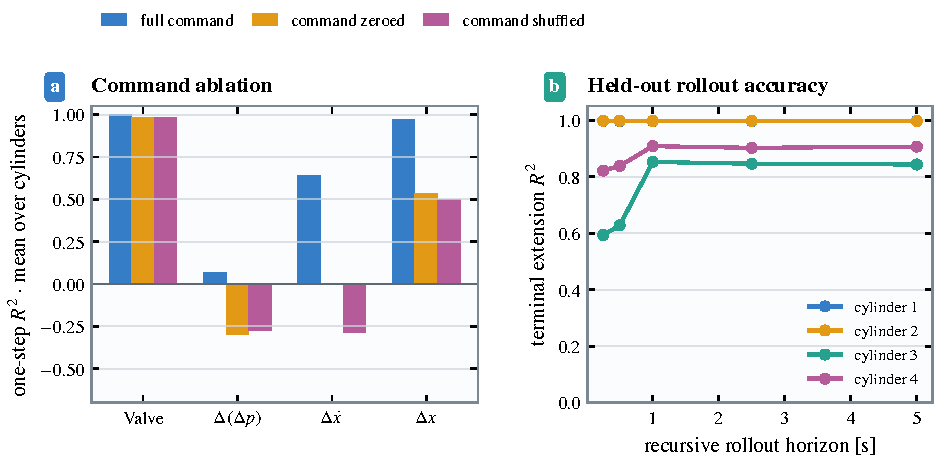
\includegraphics[width=\textwidth]{images/ch5_rom_validation}
  \caption{Offline validation of the command ROM on held-out runs.
  (a)~One-step $R^2$ per output group, averaged over the four cylinders, with
  the full desired command, with the command zeroed, and with the command
  shuffled across the batch. The collapse of the velocity and extension scores
  without the true command demonstrates command authority. (b)~Terminal
  extension $R^2$ of recursive rollouts up to $\unit[5]{s}$, shown separately
  for each cylinder so coincident high-accuracy traces remain visible.}
  \label{fig:models:rom-validation}
\end{figure}

\subsection{Closed-Loop Calibration Against the Deployment Plant}
\label{sec:models:rom-calibration}

The Simscape-trained ROM has a systematic extension offset when driving PhysX.
The promoted checkpoint adds a bounded, command-gated correction:
%
\begin{equation}
  \label{eq:models:rom-correction}
  \hat{x}_{i,k+1} \leftarrow \hat{x}_{i,k+1} + \delta_i(\bm{h}_k, \bm{c}_k),
  \qquad |\delta_i| \leq \unit[3]{mm},
  \qquad \delta_i\big|_{\bm{c}_k = \bm{0}} = 0,
\end{equation}
%
It is trained on $4\,084$ IsaacLab transitions from five reachable reference
shapes, with Simscape replay. All hydraulic and integration parameters remain
frozen. The gate sets the correction to zero for a commanded hold.

The calibrated command ROM serves as the deployment plant in
Section~\ref{sec:sys:rom-is-plant}. Unlike the ID--FD path, it has seen PhysX
data. It is frozen and has no latent input; adaptation modifies only the inverse
path.

\section{The Privileged Latent and Its Limits}
\label{sec:models:latent}

The system-dynamics model is an analysis model, not an actuator. It approximates
the command-ROM--PhysX plant and tests whether a compact factor-dependent
context improves prediction. It is trained from scratch on the IsaacLab data
of Section~\ref{sec:data:isaaclab}.

At each $\unit[50]{ms}$ step, the model predicts the next 12-dimensional
hydraulic-state increment from the observable state, joint context, consecutive
commands $[\bm{u}_{k-1},\bm{u}_k]$ and a six-tick causal belief. Training uses a
five-transition unroll. The matched control $SD_0$ has the same structure but
no latent input.

The privileged encoder $\bm{z}=\mu(\bm{e})$ maps the six physical factors to two
dimensions and is trained jointly with $SD_z$. At a 20-tick horizon, the true
latent is compared with zero, shuffled, random, mean and nominal controls using
paired bootstrap intervals on validation and reserved-test runs.

The true latent reduces pooled rollout error by $7.20\times10^{5}$ on 20
validation runs ($95\,\%$ interval
$[-1.03\times10^{6},-4.30\times10^{5}]$) and by $4.41\times10^{5}$ on 16 test
runs ($[-7.61\times10^{5},-1.74\times10^{5}]$).

The per-channel result is narrower (Table~\ref{tab:models:latent-channels}).
The significant gain is confined to pressure; extension and velocity intervals
cross zero on both pools. These are the channels used by the controller.

Figure~\ref{fig:models:sd-architecture} shows the two conditioning paths and
the transition model. The privileged factor encoder is used during training;
the belief GRU uses only causal state-action history.

\begin{figure}[H]
  \centering
  \includegraphics[page=4,width=\textwidth]{images/ch5_network_architectures}
  \caption{System-dynamics surrogate. The transition model combines a
  two-dimensional static plant context and a 16-dimensional causal dynamic
  belief with the hydraulic state, consecutive valve commands and joint
  context. A three-layer, 256-wide MLP predicts the transition; training uses
  a five-step unroll.}
  \label{fig:models:sd-architecture}
\end{figure}

\begin{table}[H]
  \centering
  \caption{Per-channel decomposition of the paired latent advantage at a
  $20$-tick horizon, pooled over $36$ runs. Values are the mean paired
  difference between the latent-conditioned model and the no-latent control,
  with a $95\,\%$ bootstrap interval; a negative value favours the latent for
  the pooled state error, and a positive value favours it for the per-channel
  errors as signed here. The advantage is confined to the pressure channel.}
  \label{tab:models:latent-channels}
  \begin{tabular}{lccc}
    \toprule
    Channel & mean paired difference & $95\,\%$ interval & excludes zero \\
    \midrule
    extension & $5.2\times10^{-5}$ & $[-3.6\times10^{-5},\; 1.4\times10^{-4}]$ & no \\
    velocity  & $-2.4\times10^{-4}$ & $[-7.1\times10^{-4},\; 2.4\times10^{-4}]$ & no \\
    pressure  & $1.75\times10^{5}$ & $[2.1\times10^{4},\; 3.3\times10^{5}]$ & yes \\
    \bottomrule
  \end{tabular}
\end{table}

Thus the two-dimensional context contains held-out hydraulic information, but
this test does not establish AAM accuracy or control improvement. It compares
separately trained models; the within-model latent substitution in
Section~\ref{sec:eval:predictive-utility} isolates latent input and also finds
extension and velocity sensitivity. The main limitation is that the strongest
signal lies in pressure, which the controller does not integrate.

The encoder, $SD_z$, belief module, normalisers, input mask, split and rollout
protocol are then frozen for downstream use.

\section{Arm Adaptation Module}
\label{sec:models:aam}

The AAM estimates $\hat{\bm{z}}=\mathrm{AAM}(\bm{H}_t)$ from deployment
history. Each row contains five joint positions, five joint velocities, four
cylinder pressure differences and four previous valve commands. A four-layer,
width-64 causal convolution processes 20 rows ($\unit[1.0]{s}$, 360 values).

The pressure values are recursive actuator-model states, not measurements:
they come from the command ROM in \ppoROM{} and the frozen FD in
\ppoAAMIDFD{}. The factor vector, true latent, reference, future rows and hidden
state are excluded. Using the previous valve command keeps each row causal.
Validation selected the shortest competitive history from $5$, $10$, $20$ and
$40$ ticks. Latent RMSE is $0.802$ on validation and $0.734$ on reserved test.

Inference runs at $\unit[20]{Hz}$ inside the $\unit[60]{Hz}$ control loop. The
adapter is bypassed until 20 rows are available. A causal five-prediction rolling
mean adds $\unit[250]{ms}$ lag. Reported results use this online smoother, not
the earlier non-causal full-run average.

\subsection{Information Content of the Estimated Latent}
\label{sec:models:aam-content}

Linear decoding from the per-run mean estimate gives $R^2=0.956$ for seal
condition, $0.448$ for compliance, $0.114$ for flow, $0.081$ for supply
pressure, $0.056$ for centre-of-mass offset and $-0.008$ for mass. The latent
therefore represents mainly seal condition. It is stable within a run but does
not refine over time.

Low-dimensional adapters can lose information when factors act through
different channels~\cite{liu2025frma}. This differs from the rapid-motor-
adaptation assumption that only task-relevant factor directions need to be
retained~\cite{kumar2021rma}: here the dominant seal-condition direction acts
through pressure, which the controller does not integrate. Estimating named
physical quantities would improve interpretation but requires an explicit
plant model~\cite{hu2026bayesian}.

\section{Latent-Conditioned Inverse-Model Adapter}
\label{sec:models:adapter}

The frozen ID produces $\bm{u}_{\mathrm{base}}=\mathrm{ID}(\bm{s},\bm{r})$.
The adapter adds a bounded latent-conditioned residual:
%
\begin{equation}
  \label{eq:models:adapter}
  \bm{u} = \operatorname{clip}\bigl(
    \bm{u}_{\mathrm{base}} + g_\psi(\bm{s}, \bm{r}, \bm{u}_{\mathrm{base}},
    \hat{\bm{z}})\bigr).
\end{equation}
%
Training minimises valve-command MSE at the exact ROM tick, with the residual
bounded to $0.15$. The ID, FD and policy are frozen during adapter training.
The \ppoAAMIDFD{} policy is separately latent-conditioned, so disabling the
residual restores the baseline actuator path but not the baseline actor. This
provides the single-variable adapter ablation used in
Chapter~\ref{chap:evaluation}.

Figure~\ref{fig:models:aam-architecture} shows the causal convolutional stack
and the bounded adapter that consumes its estimate. The upper part is the AAM;
the lower part shows where adaptation enters the frozen inverse-model path.

\begin{figure}[H]
  \centering
  \includegraphics[page=5,width=\textwidth]{images/ch5_network_architectures}
  \caption{AAM and bounded ID adapter. Four causal convolutional blocks map a
  20-step history of 18 observable features to the compact latent
  $\hat{\bm{z}}\in\mathbb{R}^2$. The adapter combines this estimate with the ID
  inputs and adds a limited, bounded correction to the frozen valve command.}
  \label{fig:models:aam-architecture}
\end{figure}

\subsection{Open-Loop Evidence}

The residual cap is $0.15$, and the frozen ID already explains about $84\,\%$
of valve-command variance (Section~\ref{sec:models:id-trust}). The adapter can
therefore make only small corrections. Section~\ref{sec:eval:predictive-utility}
tests latent information without this ceiling.

Three matched adapter arms use a zeroed, estimated or privileged latent. Across
five seeds, both latent arms improve validation loss over the zeroed arm in
$5/5$ cases. Mean paired improvements are $0.0037$ for the privileged latent
and $0.0118$ for the AAM estimate. The effect is consistent but small.

Masking pressure and force does not strengthen the result: the privileged
latent helps in only $2/5$ seeds and variance increases by about one order of
magnitude. The earlier single-seed improvement is not reproducible.

\subsection{Closed-Loop Evidence and Its Bound}
\label{sec:models:adapter-null}

Closed-loop ablations compare the full stack with zeroed, shuffled, frozen and
mean latents, plus a sham plant change. None consistently improves lateral
error, cut-height error or impacts.

Valve saturation limits the test: cylinder 1 is saturated for about $92\,\%$ of
the scored window, cylinder 2 for $67$--$82\,\%$, and cylinder 4 for
$50$--$57\,\%$. Control-effort ratios before and after the plant change are
$1.005$--$1.009$. A bounded additive correction has little authority under
these conditions~\cite{sofrony2024antiwindup}.

Reducing the lead cap lowers cylinder-1 saturation from $0.91$ to $0.14$ but
triples cut-height error. The task is therefore close to the plant capability
limit (Section~\ref{sec:sys:capability}).

\subsection{Propagation of the Latent Advantage}
\label{sec:models:chain}

The chain gate compares
$SD_0(\bm{s},\bm{u})$, $SD_z(\bm{s},\bm{u},\bm{z})$ and
$SD_z(\bm{s},\bm{u},\hat{\bm{z}})$ under the frozen protocol with paired
bootstrap intervals. Neither the true nor estimated latent improves extension
or velocity over $SD_0$ with an interval excluding zero. The estimate is not
worse than the true latent, so estimation is not the limiting stage. The
measurable advantage remains in pressure (Table~\ref{tab:models:latent-channels}).

Section~\ref{sec:eval:predictive-utility} finds the estimate comparable with the
privileged latent within one model, confirming that the AAM is not the main
loss. The missing link is a path from pressure information to the integrated
extension command with sufficient actuator headroom. Chapters~\ref{chap:evaluation}
and~\ref{chap:conclusion} examine this limit.

\section{Training and Model-Selection Protocol}
\label{sec:models:training}

Adaptation data are split $82/20/16$ into training, validation and reserved
test by complete run and factor configuration; windows do not cross run
boundaries. The 16 test runs are not used for model or hyperparameter selection.
$SD_z$ and $SD_0$ are selected on validation rollout, the AAM on downstream
rollout, and the adapter on validation command error. Table~\ref{tab:models:frozen}
records the selected checkpoints.

\begin{table}[H]
  \centering
  \caption{Provenance of each model in the adaptation chain. Frozen components
  are loaded unchanged and never receive gradients in this chapter.}
  \label{tab:models:frozen}
  \small
  \begin{tabular}{lll}
    \toprule
    Model & Status & Selected checkpoint \\
    \midrule
    Control ID            & frozen  & paired-control, Section~\ref{sec:models:id} \\
    Strict FD             & frozen  & strict-excitation, Section~\ref{sec:models:fd} \\
    Command ROM           & frozen  & PhysX-calibrated, Section~\ref{sec:models:rom-calibration} \\
    $SD_0$ (no latent)    & scratch & epoch $58$ \\
    $SD_z$ + encoder      & scratch & epoch $48$, frozen after the gate \\
    AAM                   & scratch & epoch $73$, $\unit[1.0]{s}$ causal CNN \\
    Latent adapter        & scratch & epoch $116$ \\
    \bottomrule
  \end{tabular}
\end{table}

The deployed adapter is trained and selected on recorded valve-command error.
This avoids the objective mismatch of an earlier next-state-loss variant. Each
component is evaluated on its stated training contract.

\RRLABchapterblank
%%%%%%%%%%%%%%%%%%%%%%%%%%%%%%%%%%%%%%%%%%%%%%%%%%%%%%%%%%%%
%% Chapter 6 - Control Framework and Simulation Integration
%% (12-18 pages)
%% Purpose: specify the complete controller and present the THREE
%% control stacks as one controlled experiment rather than a
%% collection of disconnected models.
%% Main output: reproducible control architecture, policy task
%% definition, integration details, and the matching rules that make
%% the three-way comparison fair.
%%
%% NOTE ON NOMENCLATURE: the only stack names are PPO-ROM (R),
%% PPO-ID-FD (IF) and Adaptive Forward (AF). The earlier PPO1/PPO2 and
%% PPO1-A/B, PPO2-A/B/C/D labels are superseded and must not reappear,
%% and neither must AF or PPO-(AAM)-ID-FD.
%% The BASE policy is NOT a residual policy: it emits its command
%% directly and no nominal command is added at runtime. AF adds a
%% bounded term around that frozen base, but this is an online
%% adaptation mechanism internal to the RL policy, NOT residual RL in
%% the sense of correcting a classical controller: no analytic
%% controller runs underneath at deployment.
%%%%%%%%%%%%%%%%%%%%%%%%%%%%%%%%%%%%%%%%%%%%%%%%%%%%%%%%%%%%
\chapter{Control Framework and Simulation Integration}
\label{chap:control}

Chapter~\ref{chap:models} left three actuator representations, each with its own
contract and offline evidence. This chapter puts a controller in front of them
and turns them into three experiments.

Section~\ref{sec:ctrl:dls} describes the classical controller, because it is
where the competence comes from even though it never runs at deployment.
Section~\ref{sec:ctrl:ppo} specifies the policy: what it sees, what it emits,
what stops it from emitting something dangerous, and what it is paid for.
Section~\ref{sec:ctrl:training} explains how the first becomes the second, and
reports a result about that transfer which changed the training protocol of this
thesis. The individual stacks appear only after those three are fixed.

\section{The DLS Teacher and Its Two Roles}
\label{sec:ctrl:dls}

\subsection{Scope and Role of the Controller}

No damped-least-squares layer runs underneath the policy at runtime and
nothing is added to the policy's output; if the policy emits zero, the arm does
not move. The DLS controller is nevertheless the reason the policies work at
all, and it appears twice, both times at training or collection time and never
at deployment (Figure~\ref{fig:ctrl:teacher-student}). It is the
\emph{privileged teacher} whose behaviour the policies are distilled from
(Section~\ref{sec:ctrl:training}), and it is the closed-loop controller that
drove the identification runs of Section~\ref{sec:data:isaaclab}. Calling it a
nominal layer would misdescribe the deployed system and would make every
reported result a property of a controller pair rather than of the policy.

\begin{figure}[tb]
  \centering
  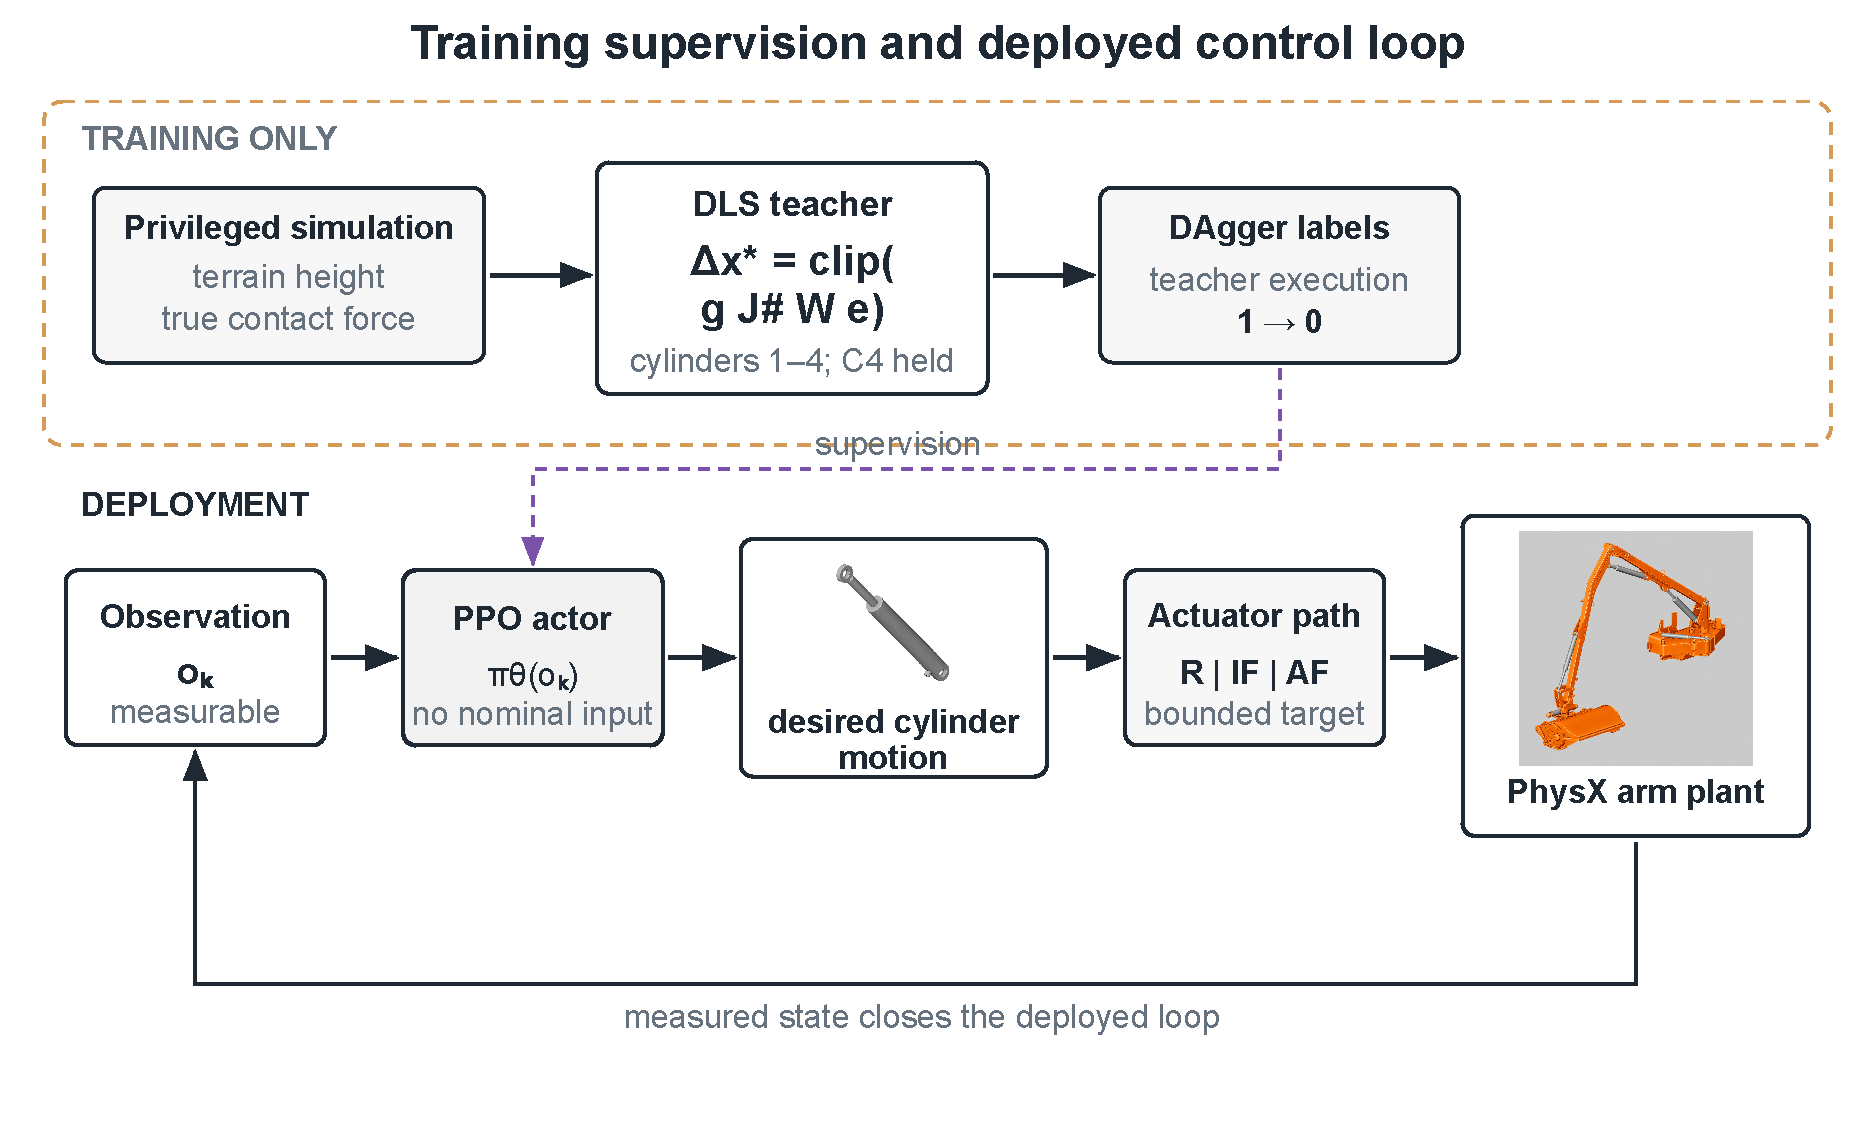
\includegraphics[width=\textwidth]{images/ch6/ch6_teacher_student}
  \caption{Training supervision and deployment. Simulator-only terrain and
  contact signals drive the DLS teacher, which supplies DAgger labels to the
  actor. At deployment only the lower feedback loop remains: measured
  observations pass through the PPO actor, the shared cylinder interface and
  the selected R, IF or AF actuator path before PhysX updates the arm. No
  nominal command is added to the policy output.}
  \label{fig:ctrl:teacher-student}
\end{figure}

\subsection{Privileged Information}

The teacher is \emph{privileged} rather than better tuned: it reads two
quantities that no deployable controller on this machine could obtain, namely
the exact terrain height directly under the cutter, queried from the simulator
rather than inferred from a forward-looking scan, and the true cutter--ground
contact force. Together these turn the hardest part of the task, knowing where
the ground is underneath a $\unit[1.2]{m}$ flail head that is occluding it,
into a lookup.

The teacher uses that privilege in a specific way. Rather than commanding a
height, it runs a contact regulator: it maintains a vertical offset relative to
the ground and adjusts that offset to hold the measured contact force near
$\unit[250]{N}$ within a $\unit[100]{N}$ deadband, pressing down below the band,
backing off proportionally above it, searching downward when contact is lost
and retreating immediately on a force spike. The accumulated offset is clamped
to $[-0.30, -0.05]\,\mathrm{m}$ so the regulator can neither drive the head into
the ground nor lift it clear.

The teacher's advantage is therefore not kinematic. Its inverse is the same DLS
solution available to anything; what it has is contact sensing, and that is the
quantity the student must infer from a noisy forward scan and its own contact
history.

\subsection{From Task Error to Cylinder Command}

The rest of the teacher is conventional and is stated for completeness. A goal
point is maintained in the truck frame: laterally it tracks the verge centre
line, vertically it follows the measured ground height plus the contact
regulator's offset. The task error is the difference between that goal and the
measured cutter position, with the lateral component weighted by a factor of
three, because on this machine lateral error is what the acceptance gate
measures and vertical error is largely handled by contact.

That error is mapped to cylinder space through the damped least-squares
inverse~\cite{wampler1986manipulator,nakamura1986inverse} of the measured cutter
Jacobian $\bm{J}_c$ of Section~\ref{sec:sys:task-jacobian},
%
\begin{equation}
  \label{eq:ctrl:teacher-dls}
  \begin{aligned}
    \bm{J}_c^{\#}(\lambda)
      &= \bm{J}_c^{\mathsf T}
         \left(\bm{J}_c\bm{J}_c^{\mathsf T}
               + \lambda^2\bm{I}\right)^{-1}, \\
    \Delta\bm{x}^{*}_{1:3}
      &= \operatorname{clip}\Bigl(
          g\, \bm{J}_c^{\#}(\lambda)\, \bm{W}\bm{e},\;
          \pm\, \Delta x_{\max}\Bigr),
      \quad g = 0.30,
      \quad \Delta x_{\max} = \unit[3]{mm}.
  \end{aligned}
\end{equation}
%
with $\bm{W}$ the lateral weighting and the per-step clamp bounding how far any
cylinder may be asked to move in one tick. Only cylinders~1--3 are solved.
Cylinder~4 is held at the reference extension that keeps the head down, for the
reason given in Section~\ref{sec:sys:platform}. The gain $g$ is small on
purpose: this is a stiff, heavy mechanism in contact, and a resolved-rate
controller that closes quickly on the task error simply excites it.

\begin{figure}[tb]
  \centering
  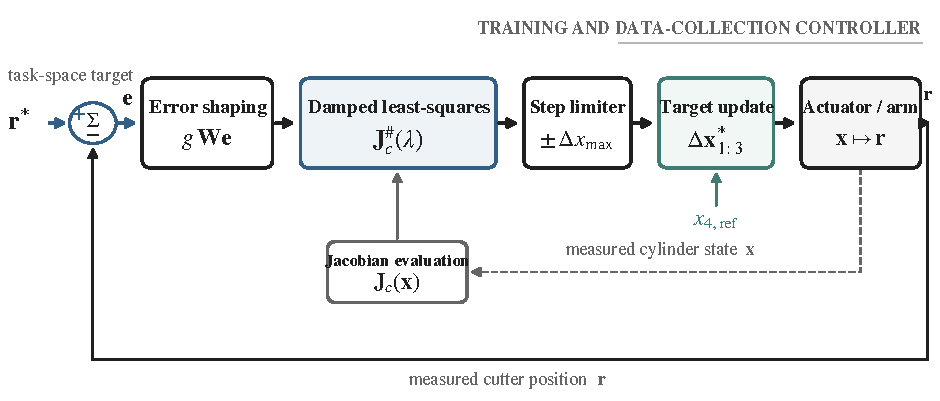
\includegraphics[width=\textwidth]{images/ch6/ch6_dls_controller}
  \caption{Feedback realisation of the damped least-squares teacher of
  \eqref{eq:ctrl:teacher-dls}. The weighted task error is scaled by $g$, mapped
  to the first three cylinder coordinates by the measured damped inverse
  $\bm{J}_c^{\#}(\lambda)$, and clipped to $\pm\Delta x_{\max}$ per tick. Cylinder~4 is
  held at its head-down reference. Cutter position closes the task-space loop
  and the measured cylinder state updates $\bm{J}_c$ at every step. The loop is
  used only for teaching and data collection, never at deployment.}
  \label{fig:ctrl:dls-loop}
\end{figure}


\subsection{Execution Through the Student Interface}

One implementation detail determines whether distillation converges to something
usable. The teacher's output $\Delta\bm{x}^{*}$ is not written to PhysX
directly: it is converted into the same normalised four-value action the student
emits and pushed through the student's entire action chain into the same plant,
so every label the student imitates is by construction an action it can produce.
A teacher writing targets directly to the plant would generate labels outside
the student's reachable set, giving the imitation error a floor no training
could remove.

\subsection{Teacher Performance}

Quoting the teacher's performance is necessary because distillation cannot
exceed it and the gates of Section~\ref{sec:sys:evaluation-criteria} were
anchored to it. Table~\ref{tab:ctrl:teacher} reports the privileged teacher
measured on the stage-6 verge task through the ROM plant, over 128 environments
and 480 control steps.

\begin{table}[tb]
  \centering
  \caption{The privileged DLS teacher, measured on the stage-6 verge task
  through the command-ROM plant (128 environments, 480 steps, all eleven path
  families, seed 17). It is competent, not perfect,
and several evaluation thresholds sit deliberately just outside what it achieves.}
  \label{tab:ctrl:teacher}
  \small
  \begin{tabular}{lcc}
    \toprule
    Quantity & Teacher & Gate \\
    \midrule
    Mean $|e_{\mathrm{cut}}|$        & $\unit[0.0234]{m}$ & $\leq \unit[0.040]{m}$ \\
    p95 $|e_{\mathrm{cut}}|$         & $\unit[0.1524]{m}$ & --- \\
    Mean $|e_{\mathrm{lat}}|$        & $\unit[0.1221]{m}$ & $\leq \unit[0.300]{m}$ \\
    Ground-contact fraction          & $0.7807$ & $\geq 0.700$ \\
    p01 head alignment               & $0.9638$ & $\geq 0.900$ \\
    Minimum head alignment           & $0.8317$ & --- \\
    p95 tool acceleration            & $\unit[64.9]{m/s^2}$ & $\leq \unit[120]{m/s^2}$ \\
    \bottomrule
  \end{tabular}
\end{table}

The teacher is competent but visibly imperfect: it loses ground contact about a
fifth of the time and its cut-height tail is six times its mean. This is why
Section~\ref{sec:sys:evaluation-criteria} re-derived several thresholds, since a
gate set above these numbers could not be passed by the ground-truth controller
itself and would carry no information about the policy.

\section{Policy Formulation}
\label{sec:ctrl:ppo}

\subsection{Policy Definition}

The deployed controller is a memoryless Gaussian multilayer perceptron mapping
a $66$-value observation to four normalised actions. Actor and critic are
separate networks with hidden widths $256$--$128$--$64$, ELU activations and
empirically normalised observations. PPO~\cite{schulman2017proximal} is supplied
by RSL-RL~\cite{rudin2022learning}. This base policy is shared by all three
stacks; \ppoAAMFD{} freezes it and widens the actor input by four plant-context
columns, of which only the payload channel carries information here
(Section~\ref{sec:ctrl:af-residual}).

The four actions denote desired cylinder increments in R and IF and valve
commands in AF (Section~\ref{sec:ctrl:af-fd-sufficient}). The base policy has no
nominal controller beneath it, and the truck's forward motion remains scripted.

\subsection{The Observation Vector}

Figure~\ref{fig:ctrl:observation} lays out the $66$ channels by group. The
grouping tells the story of what this controller has to reason about: nine
terrain-height samples ahead of the cutter, three task-error channels, sixteen
channels of cylinder state and remaining travel, sixteen describing the
actuator interface, ten of pose and context, and twelve of model error.

\begin{figure}[tb]
  \centering
  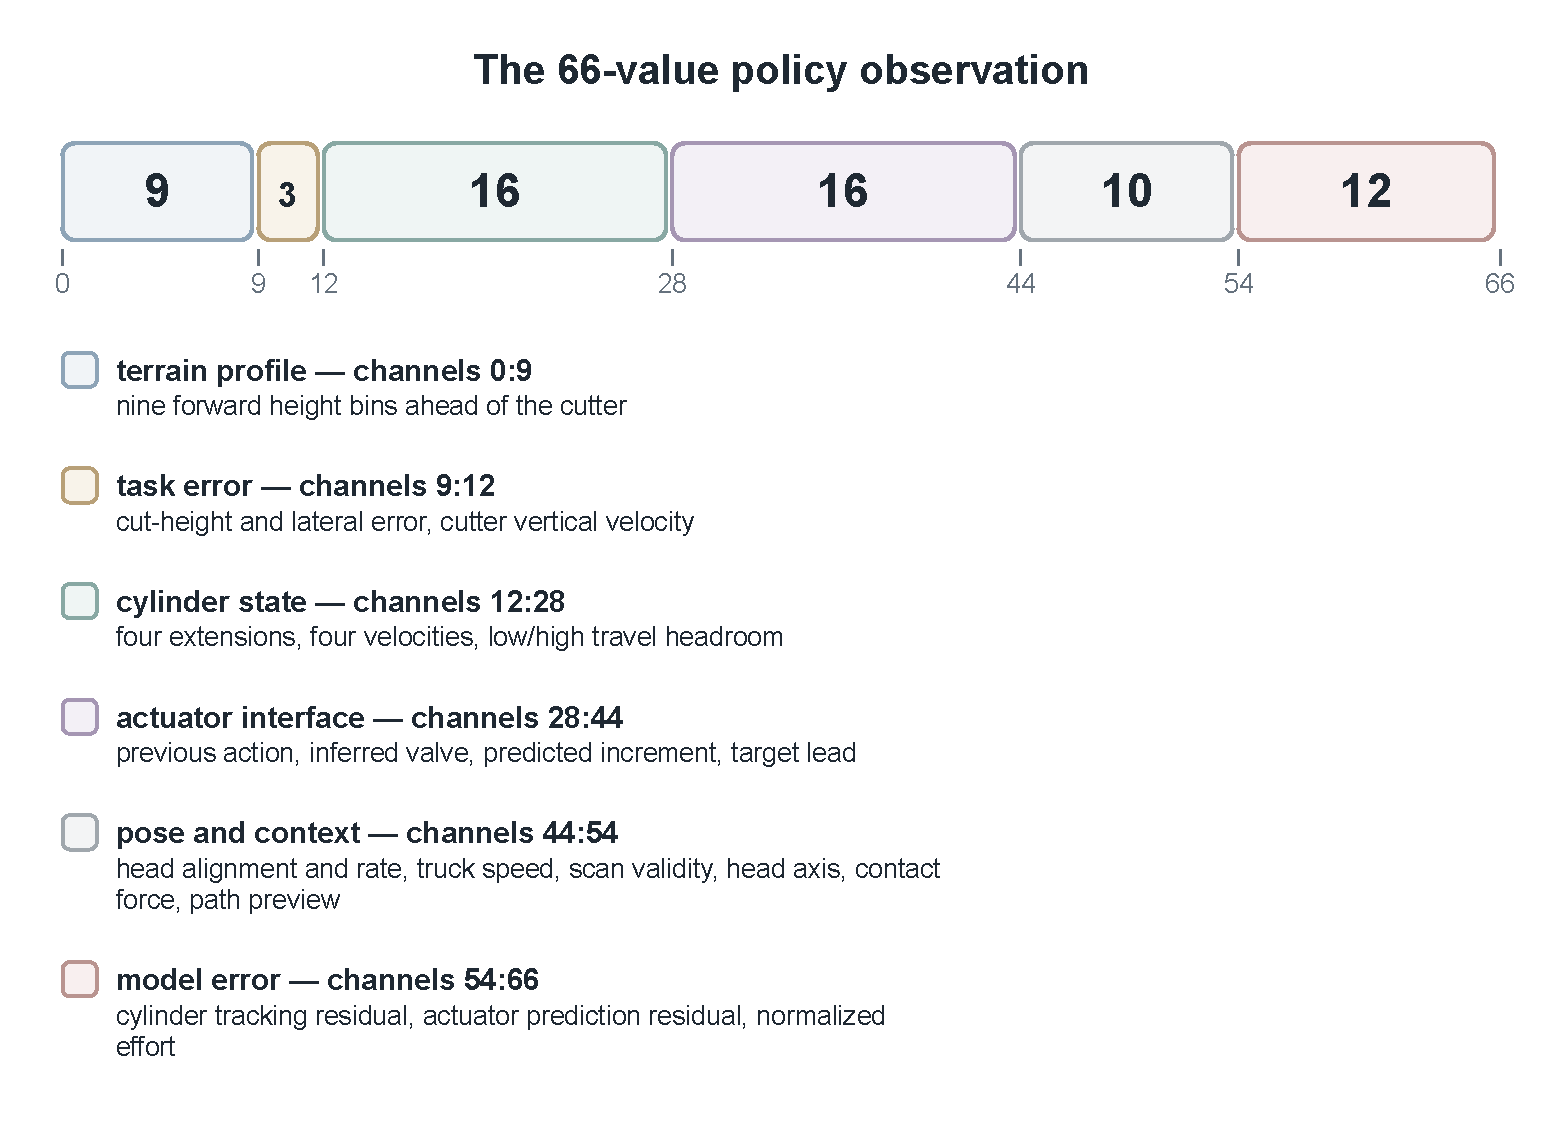
\includegraphics[width=\textwidth]{images/ch6/ch6_observation}
  \caption{The policy observation contract. The six coloured groups form the
  $66$-channel task input shared by R, IF and AF. AF appends the four white
  plant-context inputs in the slice $66{:}70$; only payload varies in the
  reported campaign.}
  \label{fig:ctrl:observation}
\end{figure}

The last twelve channels carry cylinder tracking residual, actuator prediction
residual and normalised effort. A memoryless network cannot form these temporal
errors from one observation, and without them the error to be corrected is
absent from its input. Across ten training blocks, p01 head alignment remained
at $0.79$--$0.80$ when only the feedforward source or levelling gain changed.

This shared contract also limits attribution. The tracking residual is near zero
under R but carries the ID--FD path's standing error under IF, giving IF a useful
closed-loop correction signal. The R--IF comparison therefore cannot separate
the actuator representation from the value of that signal.

\subsection{The Action and Its Bounds}

The policy emits $\bm{a} \in \mathbb{R}^4$, sampled from its Gaussian at
training time and taken at the mean for evaluation. Five bounding stages sit
between that sample and the PhysX cylinder target
(Figure~\ref{fig:ctrl:action-chain}). Each can only reduce authority, never
introduce motion the policy did not request.

\begin{figure}[tb]
  \centering
  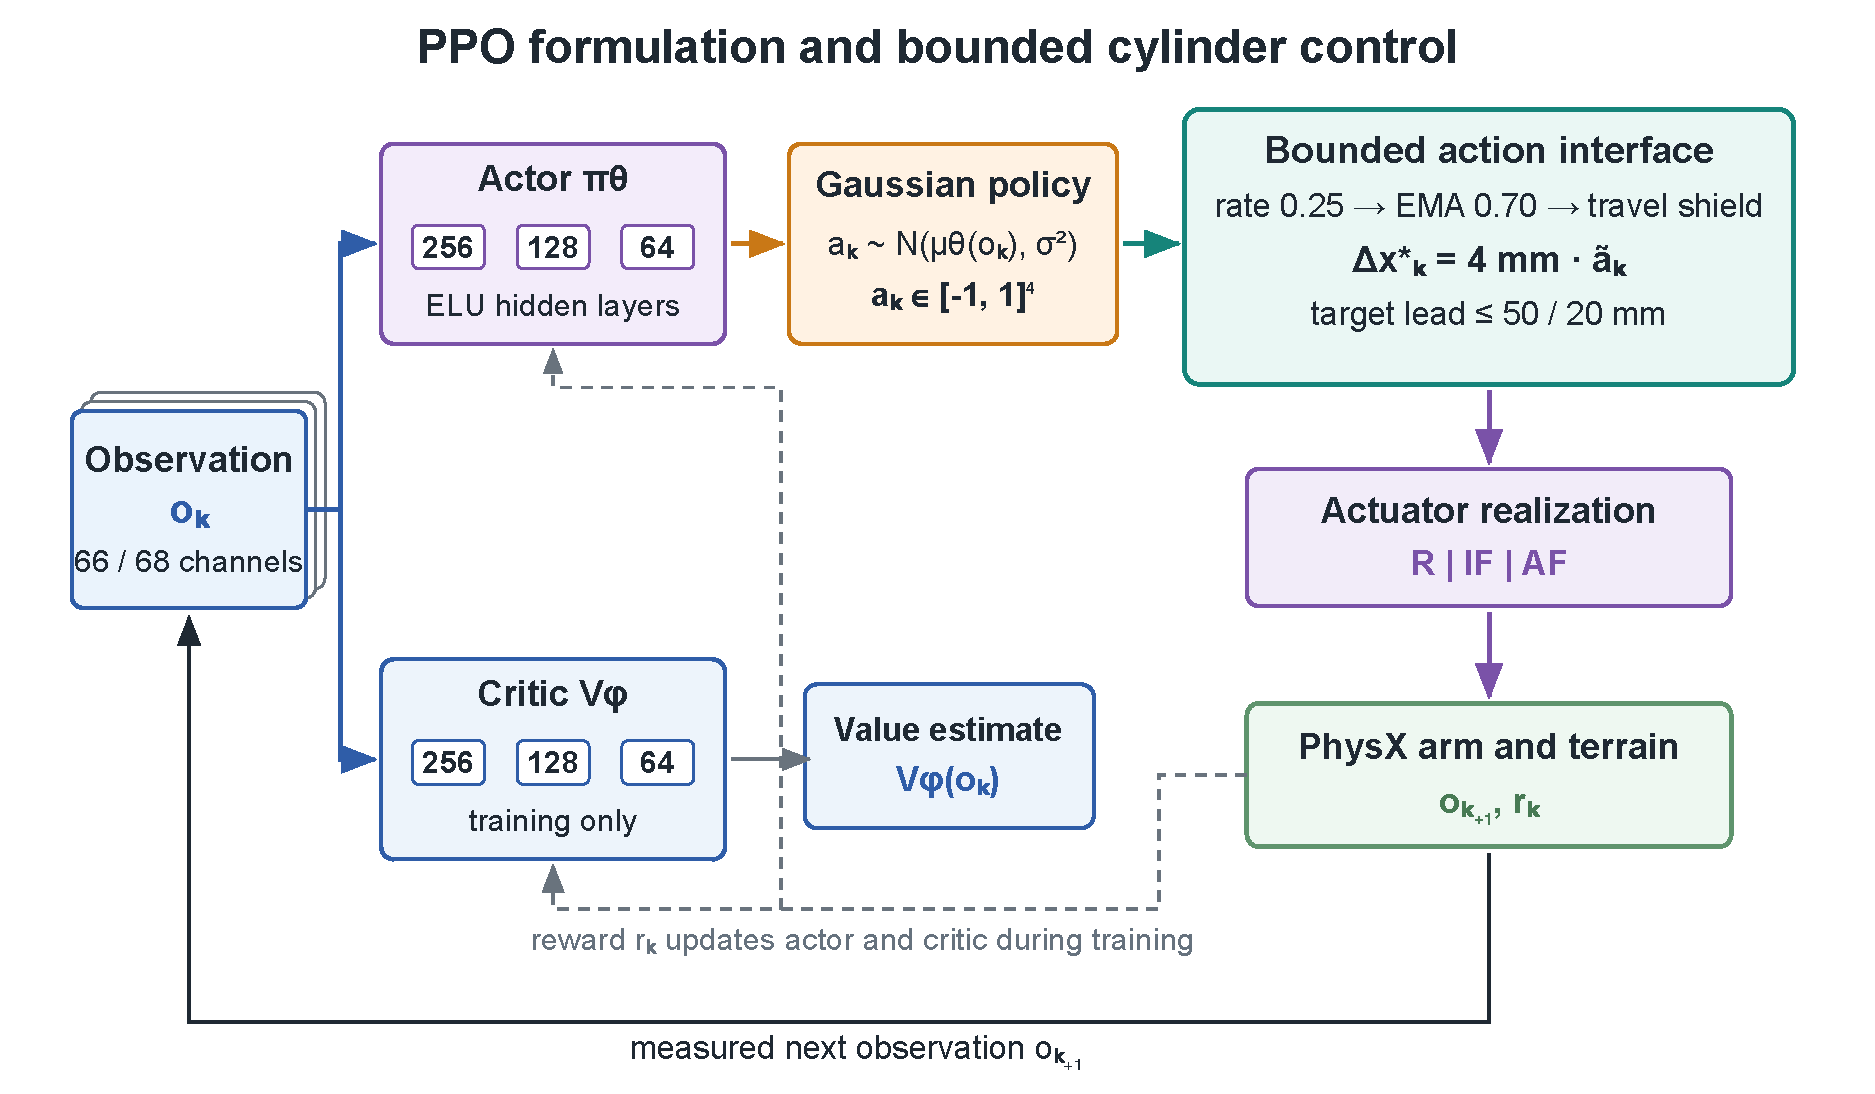
\includegraphics[width=\textwidth]{images/ch6/ch6_action_chain}
  \caption{PPO actor--critic formulation and deployed control path. The actor
  maps the observation to a four-dimensional Gaussian action. Rate limiting,
  exponential filtering, the travel shield, command scaling and the target-lead
  cap bound that action before the selected R, IF or AF actuator path drives
  the PhysX arm. The critic and reward update are training-only; measured state
  closes the deployed loop.}
  \label{fig:ctrl:action-chain}
\end{figure}

The rate limit bounds $|\Delta \bm{a}|$ at $0.25$ per control step and is held
\emph{constant} across every curriculum stage rather than used as a curriculum
knob, by the reachability argument above: the teacher's own command stream has a
structural per-step bound near $0.20$, so a student limit below that makes part
of the label set unreachable. The exponential filter ($\beta = 0.70$ at the
final stage) smooths the command. The limit shield scales the command down, and
only in the direction that consumes headroom, over the last $\unit[20]{mm}$ of
cylinder travel, replacing the teacher's hard clamp into the learned range. The
command scale converts the filtered action into $\unit[4]{mm}$ of cylinder
travel per unit action, and the target integrator accumulates the increments in
reference space, permitted to lead the measured extension by at most
$\unit[50]{mm}$ on cylinders~1 to~3 and $\unit[20]{mm}$ on cylinder~4.

This is the cylinder-increment reading of the action, used by \ppoROM{} and
\ppoIDFD{}. Under \ppoAAMFD{} the same bounded action is a valve command scaled
to span the admissible valve range, so the cylinder-space stages do not carry
the same meaning there.

The lead cap is load-bearing. Raising it to $\unit[50]{mm}$ halved lateral error
on \texttt{lane\_change\_hold} ($0.4833 \to 0.2310$) and
\texttt{boom\_sweep} ($0.3745 \to 0.1602$), but applying the same value to
cylinder~4 reduced head alignment from $0.9507$ to $0.4636$. This measured split
sets the per-axis limits above.

The chain also fixes the capability ceiling: four millimetres of cylinder travel
per step is the entire authority budget, which produces the
$\unit[0.240]{m/s}$ lateral rate limit of Section~\ref{sec:sys:capability} from
which the reference paths are derived.

\subsection{The Reward Function}

The final \ppoROM{} reward has ten bounded terms
(Table~\ref{tab:ctrl:reward}): three task rewards and seven behaviour penalties.
All retain a gradient beyond the acceptance boundary. Three rules govern them,
each adopted after a measured failure.

\paragraph{No Gaussian Shaping}
The earlier reward priced tracking as $w\exp[-(e/s)^2]$, which is effectively
flat beyond about $2s$ and therefore supplies almost no gradient where the
failing path families live. Every shaping term is instead linear or Huber in the
error. Writing $x = |e|/s$, the two shapes used are
%
\begin{equation}
  \label{eq:ctrl:shapes}
  B(e;s,c) = \min(x,\,c),
  \qquad
  H(e;s,c) = \min\Bigl(c,\;
  \begin{cases}
    \tfrac{1}{2}x^{2}, & x \le 1\\
    x - \tfrac{1}{2},  & x > 1
  \end{cases}\Bigr).
\end{equation}
%
$B$ has the same gradient at $\unit[0.5]{m}$ of error as at $\unit[0.05]{m}$,
so a policy far from the reference is still told which way to move; $H$ buys
quadratic precision near zero where cut height needs it, without a vanishing
far field.

\paragraph{Bounded Terms}
An unbounded term can dominate the sum and destabilise the critic. Each
contribution is clipped, giving the reward a published budget: $6+12+4 = 22$ for
the task terms against $-24$ for the safety terms. A non-finite value is
replaced by $-25$, just below that worst case, so a numerical fault can never
outscore legitimate behaviour.

\paragraph{Fixed Sign Convention}
The three task terms are non-negative and the seven safety terms non-positive.
This makes worst-case (CVaR) weighting~\cite{rockafellar2000cvar} safe: scaling
a non-positive term by a factor $\ge 1$ can only lower return. Earlier positive
worst-case weights instead rewarded poor environments, while an action-magnitude
penalty discouraged the sustained offsets required by three path families.

\begin{table}[tb]
  \centering
  \caption{The ten reward terms of the final \ppoROM{} task, with weights and
  shaping scales. $B$ and $H$ are the bounded shapes of
  Equation~\eqref{eq:ctrl:shapes}. The lateral and head terms each combine a
  coarse and a fine scale, so far-field correction and near-field precision are
  priced separately.}
  \label{tab:ctrl:reward}
  \small
  \begin{tabular}{llp{6.0cm}}
    \toprule
    Term & Weight & Shape and purpose \\
    \midrule
    Cut-height tracking & $+6$   & $H$, scale $\unit[0.04]{m}$, cap $2.5$; the
      primary mowing-quality term \\
    Lateral tracking    & $+12$  & $B$, coarse $\unit[1.50]{m}$ and fine
      $\unit[0.60]{m}$ mixed $0.6/0.4$; the primary line-following term \\
    Ground contact      & $+4$   & pays for the cutter being in contact \\
    Head alignment      & $-12$  & $B$ on the deficit below $0.98$, fine scale
      $0.02$ and coarse scale $1.00$ mixed evenly \\
    Contact loss        & $-3$   & charges directly for loss of contact \\
    Action rate         & $-1$   & $B$ on the mean absolute command change,
      scale $0.25$; penalizes chatter \\
    Tool acceleration   & $-1$   & $B$, scale $\unit[300]{m/s^2}$;
      mechanical-wear proxy on the cutter \\
    Contact force       & $-1$   & $B$ on force above $\unit[30]{kN}$, scale
      $\unit[150]{kN}$ \\
    Cylinder headroom   & $-2$   & $B$ on encroachment inside a
      $\unit[0.02]{m}$ margin, scale $\unit[0.10]{m}$ \\
    Hard impact         & $-4$   & indicator on the impact event \\
    \bottomrule
  \end{tabular}
\end{table}

One apparent inconsistency is deliberate. The tool-acceleration term saturates
at $\unit[300]{m/s^2}$ while its gate sits at $\unit[120]{m/s^2}$, because the
reward scale is a saturation scale for a bounded penalty rather than a target:
the gate stays the binding criterion and the reward only keeps a gradient
against gross excursions. The action-rate term is mild for a related reason,
since cylinder~4 owns head pitch and a rate tax falls hardest on the fast
corrections that keep the head down.

Every term is logged by name during training, because total reward can rise
while the system gets worse. The reward is not the result criterion; promotion
uses the eight gates of Section~\ref{sec:sys:evaluation-criteria}.

\subsection{Optimisation}
\label{sec:ctrl:optimization}

Policies are optimised with clipped-surrogate PPO over generalised advantage
estimation, in the form of Section~\ref{sec:fund:rl-residual}. The maintained
configuration uses clip parameter $\epsilon = 0.2$, discount $\gamma = 0.99$,
GAE parameter $\lambda = 0.95$, five learning epochs over four minibatches per
update, an adaptive learning-rate schedule targeting a KL divergence of $0.02$
from a base rate of $3\times10^{-4}$, gradient-norm clipping at $1.0$, and a
clipped value loss with coefficient $1.0$. The terrain task collects $32$ steps
per environment per update. At $512$ environments that is $16\,384$ transitions
per update, chosen because the inherited $128$-step horizon exceeded two
minutes per update on the available GPU without adding useful batch diversity.

The final fine-tuning blocks depart from that configuration because they run
under the reference anchor of Section~\ref{sec:ctrl:anchored} rather than an
adaptive learning-rate schedule: clip $\epsilon = 0.1$, discount
$\gamma = 0.97$, three learning epochs, fixed learning rates of $10^{-5}$ for
the actor and $10^{-4}$ for the critic, entropy coefficient $0.001$, an
exploration standard deviation fixed at $0.15$ and excluded from the gradient,
and frozen observation normalisers.

These departures reflect the locally controlled task and the anchor. The shorter
discount credits actions for the terrain state they face, the actor changes more
slowly than the critic, and the fixed learning rate avoids competing with the
explicit divergence bound. Because zero action leaves the arm stationary, early
training used a standard deviation of $0.30$ to discover command directions.
Distilled terrain policies instead use the smaller fixed value above. Exact run
values remain recorded in each frozen manifest.

\section{Training Protocol and the Distillation Finding}
\label{sec:ctrl:training}

\subsection{Distillation by DAgger}

Policies are initialised by imitation, not by reward. The privileged teacher is
rolled out in the student's own environment and the student is fitted to the
teacher's raw action by regression, in the DAgger scheme of Ross et
al.~\cite{ross2011reduction}: the teacher's probability of \emph{executing} the
action, rather than merely labelling it, is annealed from one to zero over the
first $70\,\%$ of iterations, so later training collects states the student
itself visits. Labels are accumulated in a replay buffer of $262\,144$
transitions and refitted over three epochs per iteration in minibatches of
$8\,192$.

Figure~\ref{fig:ctrl:distillation} shows a complete distillation run for the
ROM stack, taken from the stored record. The behaviour-cloning loss falls by
more than an order of magnitude while the teacher is still driving, reaches its
minimum around the handover, and then \emph{rises} once the student is alone.
That rise is the distribution shift DAgger exists to expose rather than a
failure: the student is now visiting states the teacher never chose, and the
teacher's advice on those states is new information. The closed-loop task
metrics remain near the teacher's preflight values without matching them.

\subsection{Objective Mismatch in Unconstrained Fine-Tuning}
\label{sec:ctrl:finding}

Unconstrained PPO fine-tuning from distilled checkpoints increased total reward
while degrading the primary tracking objective, in the worst case by a factor
of $12.9$. The critic remained healthy, with explained variance in the
$0.85$--$0.95$ range. This motivates the anchored formulation of
Section~\ref{sec:ctrl:anchored}, which is used for the final policies.

The reward includes ground contact and cut height as well as lateral tracking,
so it can increase while a gate-relevant tracking measure degrades. This is a
claim about two functionals over the same policy space rather than about the
optimiser. Training maximizes the expected return
$J(\vartheta)$, while acceptance is decided by the vector of physical gates
$\bm{G}(\vartheta) \preceq \bm{g}^{\star}$ of
Section~\ref{sec:sys:evaluation-criteria}. Writing
$\mathcal{F} = \{\vartheta : \bm{G}(\vartheta) \preceq \bm{g}^{\star}\}$ for the
feasible set, the measured content of the finding is
%
\begin{equation}
  \label{eq:ctrl:mismatch}
  \arg\max_{\vartheta} J(\vartheta) \notin \mathcal{F},
  \qquad\text{while}\qquad
  \vartheta_{\mathrm{distilled}} \in \mathcal{F}.
\end{equation}
%
The teacher places the distilled policy inside $\mathcal{F}$, whereas
unconstrained ascent optimises a different functional and may leave it. The
protocol therefore reports both checkpoints, logs gate metrics during training
and constrains policy drift from the point where reward and evaluation were
known to agree.

\section{Reference-Anchored PPO}
\label{sec:ctrl:anchored}

Equation~\eqref{eq:ctrl:mismatch} says that reward ascent leaves the feasible
set. It does not say that reward ascent is useless, only that it is unbounded.
The construction of this section keeps PPO and constrains how far it may travel
from a policy already known to satisfy the gates. Writing $\pi_{\mathrm{ref}}$
for a frozen reference policy and $J$ for the expected return, each training
block solves
%
\begin{equation}
  \label{eq:ctrl:constrained}
  \max_{\vartheta} J(\vartheta)
  \quad \text{s.t.} \quad
  \mathbb{E}_{\bm{o}\sim d_{\pi_\vartheta}}
  \bigl[ \mathrm{KL}\bigl( \pi_{\mathrm{ref}}(\cdot\,|\,\bm{o})
  \,\|\, \pi_\vartheta(\cdot\,|\,\bm{o}) \bigr) \bigr]
  \le \delta_{\mathrm{ref}},
\end{equation}
%
with the expectation taken over the states the policy itself visits.

\subsection{Critic Warm-Up}

After distillation the actor already behaves sensibly, but the critic has never
been fitted to the long terrain return, so the first PPO updates would move a
useful actor using a value estimate that is not yet meaningful. The actor is
frozen for $150$ iterations while only the value loss is optimised, under the
asserted invariant $\vartheta_{\text{after}} = \vartheta_{\text{before}}$. The
observation normalisers are frozen at the same point, since otherwise the same
raw observation is normalised differently from one iteration to the next and the
actor's behaviour changes while its weights do not.

\subsection{The Reference Anchor}

Let $\pi_{\mathrm{ref}}$ be a frozen copy of the accepted warm actor. It is
queried only on states the live policy visits and never supplies an executed
action, so PPO remains the sole controller of the plant. The penalty is the
\emph{forward} divergence, which for diagonal Gaussians is available in closed
form~\cite{cover2006information},
%
\begin{equation}
  \label{eq:ctrl:kl}
  D_{\mathrm{ref}}
  = \mathrm{KL}\bigl(\pi_{\mathrm{ref}} \,\|\, \pi_\vartheta\bigr)
  = \sum_i \left[
    \log\frac{\sigma_{\vartheta,i}}{\sigma_{\mathrm{ref},i}}
    + \frac{\sigma_{\mathrm{ref},i}^{2}
      + (\mu_{\mathrm{ref},i}-\mu_{\vartheta,i})^{2}}
      {2\sigma_{\vartheta,i}^{2}}
    - \frac{1}{2}\right],
\end{equation}
%
at the cost of one additional forward pass and no sampling. Because both scales
are fixed at $\sigma = 0.15$, this collapses to a pure quadratic on the drift of
the commanded action,
%
\begin{equation}
  \label{eq:ctrl:kl-fixed}
  D_{\mathrm{ref}}
  = \sum_i \frac{(\mu_{\mathrm{ref},i}-\mu_{\vartheta,i})^{2}}{2(0.15)^{2}},
\end{equation}
%
which is the second reason for fixing $\sigma$: with a free standard deviation,
entropy collapse shrinks $D_{\mathrm{ref}}$ while the commanded action moves, so
the constraint would report compliance during the drift it exists to prevent.

Forward KL penalises abandoning any reference behaviour; reverse KL could
collapse onto a subset, reproducing the observed trade between competencies.
The term is therefore a behaviour-cloning anchor on the live policy's states,
following demonstration-regularised policy gradient~\cite{rajeswaran2018dapg}.

The actor objective is
%
\begin{equation}
  \label{eq:ctrl:anchored-loss}
  \mathcal{L}(\vartheta)
  = \mathcal{L}_{\mathrm{PPO}}
  + \mathcal{L}_{V}
  - \beta\,\mathcal{H}(\pi_\vartheta)
  + \lambda_{\mathrm{ref}}\,
    \mathbb{E}_k\bigl[\mathrm{KL}(\pi_{\mathrm{ref}} \| \pi_\vartheta)\bigr],
  \qquad
  \lambda_{\mathrm{ref}} = 0.10 .
\end{equation}

\subsection{Trust Regions and Rollback}

A penalty is not a constraint: at a fixed coefficient, a sufficiently large
advantage always buys its way past. Feasibility is therefore also verified on the update taken. Two bounds are imposed,
%
\begin{equation}
  \label{eq:ctrl:bounds}
  D_{\mathrm{update}} = \mathrm{KL}(\pi_{\mathrm{old}} \| \pi_\vartheta)
  \le 0.01,
  \qquad
  D_{\mathrm{ref}} \le 0.05,
\end{equation}
%
and they do different work. $D_{\mathrm{update}}$ is the classical step-size
control that keeps the surrogate a valid local model of $J$.
$D_{\mathrm{ref}}$ is the new object: because the anchor is \emph{fixed} within
a block rather than moving with the policy, it bounds cumulative drift. A
sequence of updates each individually satisfying $D_{\mathrm{update}}$ can
still walk arbitrarily far from feasibility, and that is the trajectory the earlier campaigns took, monotonically, with the reward rising the whole
way. Only a constraint referred to a fixed feasible point can observe it.

Enforcement is in two stages. During minibatch optimisation the epoch is
early-stopped as soon as $D_{\mathrm{update}}$ exceeds its bound, and after the
update both divergences are recomputed over the full rollout. If either bound
fails, or any quantity is non-finite, the actor and its optimiser state are
restored \emph{atomically}. On a divergence rejection the critic fit is retained
when finite, since the bounds constrain the policy rather than the value
function; on a non-finite update both networks are restored. In the final block,
five of one hundred logged updates were rejected, all on the reference bound and
none on the update bound, so the drift caught was of the kind ordinary PPO
clipping does not see.

\subsection{The Block Ratchet}

The reference is not fixed forever. Within a block it is frozen. When a
checkpoint is scored and passes the gates, it is promoted to reference,
%
\begin{equation}
  \label{eq:ctrl:ratchet}
  \vartheta_{\mathrm{ref}}^{(m+1)} = \vartheta^{\star},
  \qquad
  \vartheta^{\star} \in \mathcal{F},
  \quad
  \vartheta^{\star} \in
  B_{\delta_{\mathrm{ref}}}\bigl(\vartheta_{\mathrm{ref}}^{(m)}\bigr),
\end{equation}
%
and the actor's optimiser moments are reset, because momentum accumulated
relative to the old anchor is not meaningful relative to the new one. The
critic's are retained: it is fitting the same return, and its calibration is
expensive to rebuild.

The anchor advances only through checkpoints verified against $\bm{G}$, bringing
the evaluation criterion into training. Distillation supplies the first anchor;
the critic is warmed with actor and normalisers frozen; each later block trains
within the fixed bound, rolls back rejected updates, scores checkpoints on at
least three held-out meshes and promotes only a passing checkpoint. The last
promotion is returned. Algorithm~\ref{alg:ctrl:anchored} in
Appendix~\ref{app:anchored-ppo} gives the full procedure.



\subsection{Theoretical Status}
\label{sec:ctrl:theory}

The components are standard and citable. The bound on $D_{\mathrm{update}}$ is
conservative policy iteration and its trust-region
descendants~\cite{kakade2002approximately,schulman2015trust}; the atomic
rollback is that literature's backtracking line search reduced to a single
trial point; the penalty in Equation~\eqref{eq:ctrl:anchored-loss} is a
Lagrangian relaxation of the constrained problem~\eqref{eq:ctrl:constrained} at
a fixed multiplier, with the rollback supplying the feasibility enforcement a
fixed multiplier cannot.

What does not follow is a certificate. Bounding the divergence from a verified
policy does bound gate degradation in form, since the chain rule of KL over
trajectories, Pinsker's inequality and the boundedness of every gate metric give
$|\mathbb{E}_{\pi_\vartheta}[g] - \mathbb{E}_{\pi_{\mathrm{ref}}}[g]|
\le 2 G_{\max}\sqrt{H \delta_{\mathrm{ref}}/2}$ for a metric $g$ with
$\|g\|_\infty \le G_{\max}$ over a horizon $H$
(Appendix~\ref{app:kl-bound} derives this bound step by step). At the
production horizon of $2808$ steps and $\delta_{\mathrm{ref}} = 0.05$ the
right-hand side exceeds sixteen, which for a metric bounded in $[0,1]$ is
vacuous, and there is a further measure mismatch because the constraint is
taken under the live policy's state distribution while the chain rule requires
the reference's. The construction is therefore a principled restriction of
reward ascent to a neighbourhood of a verified policy, not a guarantee: the
gates certify each promotion.

\section{R: Reference Actuator Baseline}
\label{sec:ctrl:ppo-rom}

\ppoROM{} is the reference condition. The policy emits desired cylinder motion,
the frozen command ROM converts it to a cylinder target, and PhysX closes the
loop. The scripted truck crosses a $\unit[26]{m}$ strip at a constant speed
drawn per episode from $2$ to $\unit[7]{km/h}$; path families and terrain meshes
are distributed across environments.

It is a reference condition rather than a competitor: ROM-plus-PhysX \emph{is}
the deployment plant, so \ppoROM{}'s actuator coincides with the plant. What
that does to its tracking advantage is stated in
Section~\ref{sec:ctrl:matching}.

The policy follows the chapter's three-stage construction: distillation, frozen
actor critic warm-up and reference-anchored PPO. Checkpoints $280$--$329$ were
scored on held-out meshes against the eight gates, with worst-mesh and, where
applicable, worst-family aggregation. Chapter~\ref{chap:evaluation} reports the
common-protocol evaluation.

\section{IF: Non-Adaptive Learned Baseline}
\label{sec:ctrl:ppo-idfd}

\ppoIDFD{} subclasses the \ppoROM{} task and changes exactly one thing. The
policy still emits desired cylinder motion, but that command is now realised by
the frozen inverse model of Section~\ref{sec:models:id}, which converts it to a
valve command, followed by the frozen strict forward model of
Section~\ref{sec:models:fd}, which converts the valve command to a predicted
extension increment. PhysX receives the same bounded cylinder target as before.
Task, terrain families, meshes, observation contract, action chain, reward,
gates and the PPO update are inherited unchanged, so the actuator
representation is the only free variable between the two stacks.

\emph{Robust} here means what Section~\ref{sec:fund:domain-randomization} means
by it: trained across the randomised plant family, applying one fixed response
to whichever member it meets, with no online estimation. The policy is not blind
to plant variation, since the twelve model-error channels carry a standing
residual that is itself plant-dependent. What it lacks is any representation of
\emph{which} plant produced them.

Two properties of the composed path shape its behaviour, both established
offline. The valve command is accumulated rather than issued absolutely and is
clipped to the per-axis limits $[0.95, 0.95, 0.80, 0.80]$, so the actuator path
carries its own saturation boundary independently of the action chain. Only the
predicted extension increment is integrated; the velocity output is a
diagnostic (Section~\ref{sec:models:fd}).

The stored run manifest matches \ppoROM{} field for field on actor learning
rate, entropy coefficient, seed, terrain seed, environment count, curriculum
stage, frozen normaliser and warm-up, which is what makes the pair a controlled
comparison.

\begin{figure}[!htbp]
  \centering
  \makebox[\textwidth][c]{%
    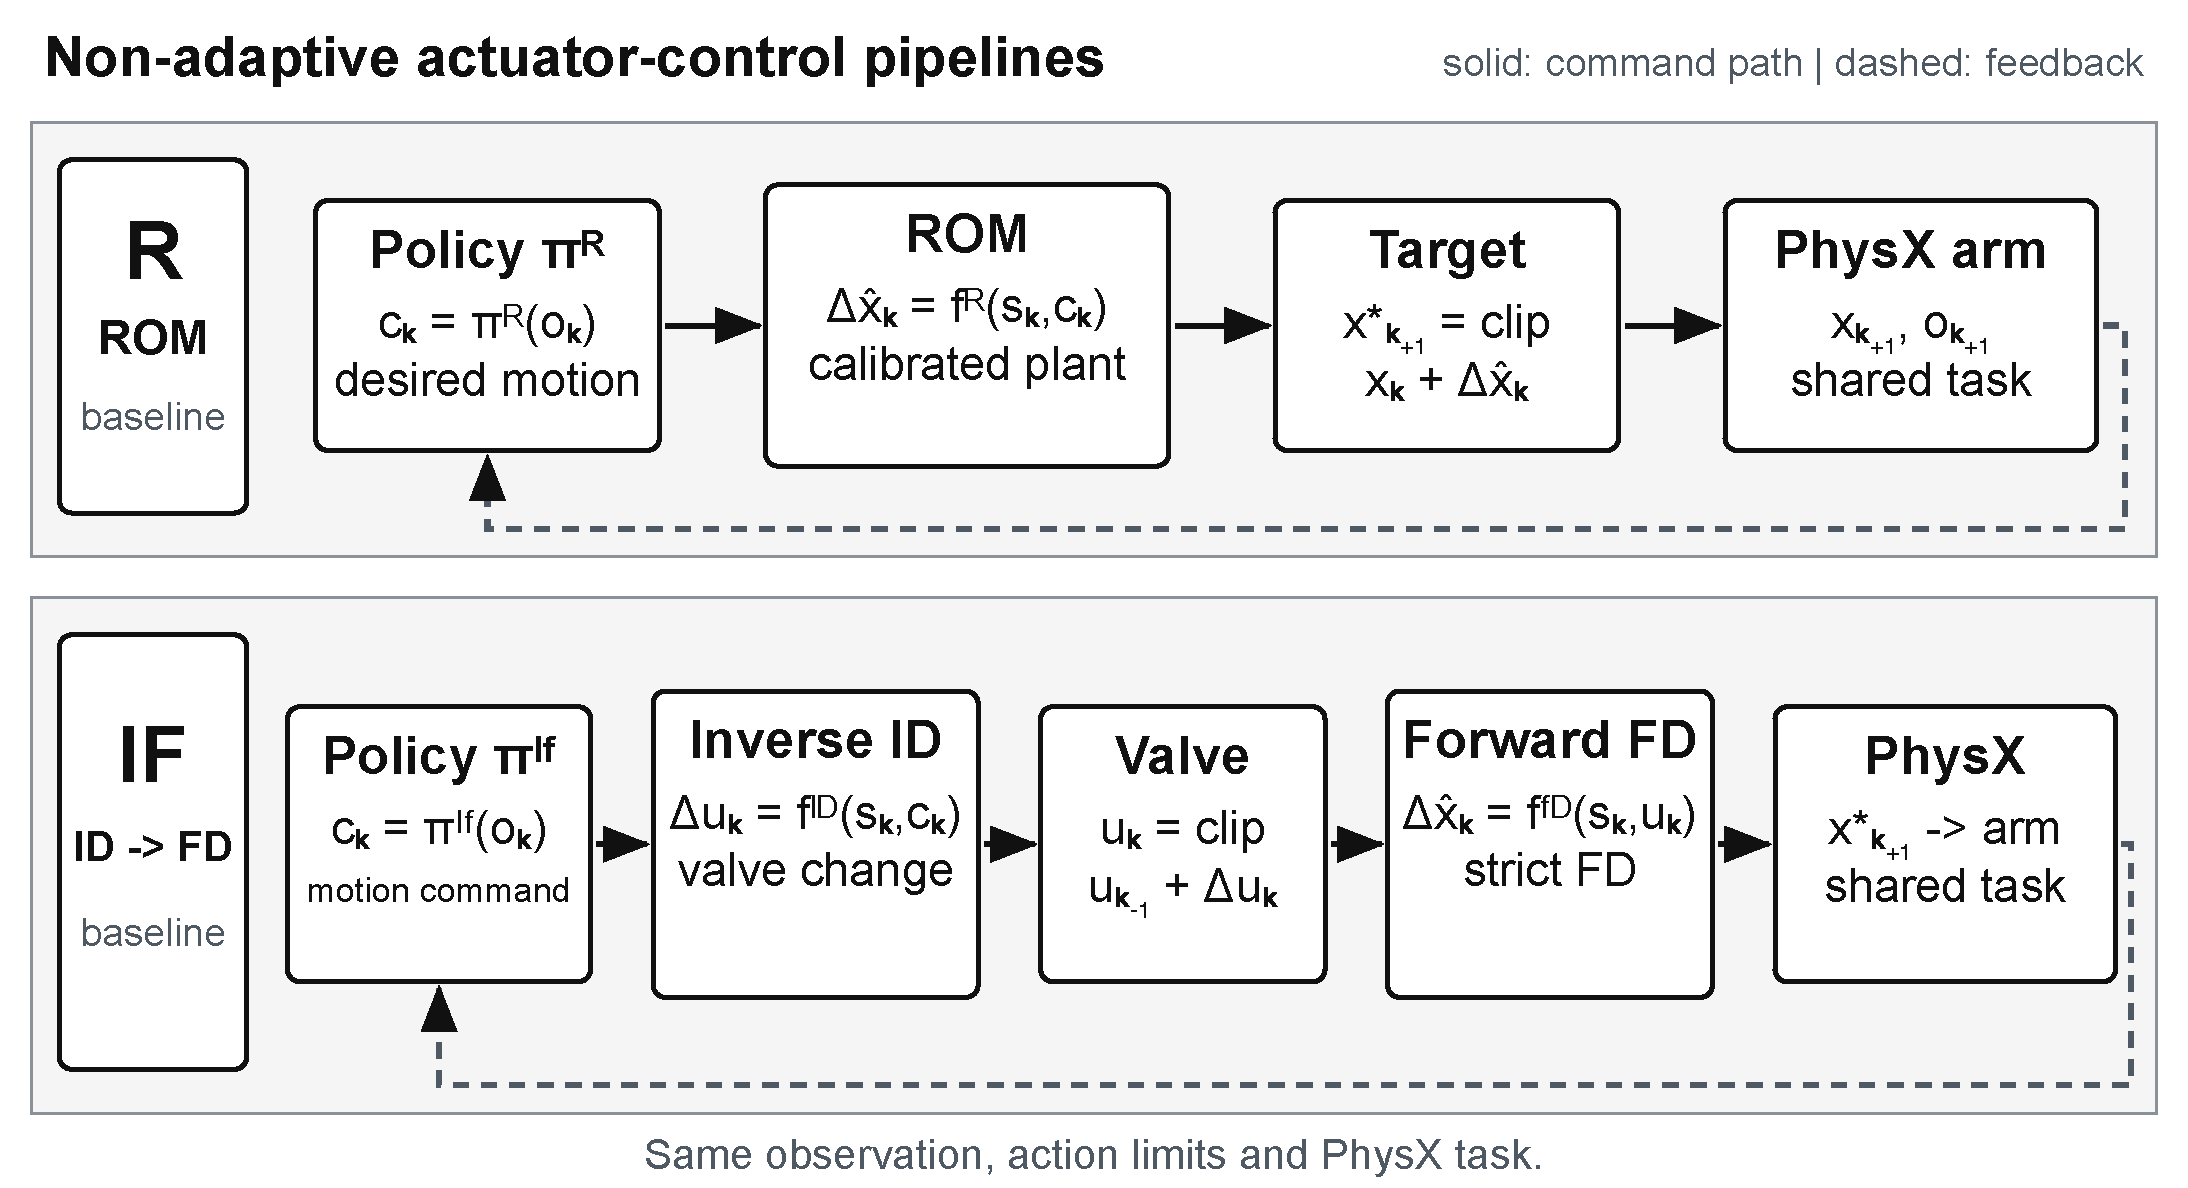
\includegraphics[width=1.08\textwidth]{images/ch6/ch6_r_if_stack}}
  \caption{The non-adaptive R and IF control pipelines. R sends the policy's
  desired cylinder motion through the calibrated command ROM. IF composes the
  independently identified inverse and strict forward models before applying
  the same bounded cylinder target in PhysX. Both paths use the same
  observation, action limits and task.}
\label{fig:ctrl:r-if-stack}
\end{figure}

\section{AF: The Adaptive Stack}
\label{sec:ctrl:ppo-aamfd}

Table~\ref{tab:ctrl:af-matching} states what AF shares with R and IF and what it
does not. AF is not a matched replacement for IF: it answers whether conditioning on an
online payload estimate can improve a frozen direct-valve controller once the
saturated inverse-model command path has been removed. The matched
actuator-representation comparison remains R against IF, and adaptation is
evaluated inside AF against its own frozen and wrong-information controls. This
is stated once here and not repeated.

\begin{table}[H]
  \centering
  \caption{What is matched between AF and the R/IF pair, and what is not.
  Section~\ref{sec:ctrl:matching} gives the full matching rules.}
  \label{tab:ctrl:af-matching}
  \small
  \begin{tabular}{@{}l c p{0.46\textwidth}@{}}
    \toprule
    Dimension & Matched? & Detail \\
    \midrule
    Task, terrain, reward, gates & yes & identical across all three stacks \\
    Base $66$-channel observation & yes & AF appends four context columns
      derived from these channels \\
    Action contract & no & AF emits the valve command directly, not a
      bounded cylinder increment \\
    Training seed & no & AF trains at a different seed \\
    Actor learning rate & no & lower than the R/IF value \\
    Frozen-actor warm-up & no & AF's base is the already-distilled policy,
      frozen; there is no separate warm-up stage \\
    \bottomrule
  \end{tabular}
\end{table}

\ppoAAMFD{} places online adaptation on the forward model alone. The policy
emits the valve command directly, the frozen strict forward model of
Section~\ref{sec:models:fd} converts that command to a predicted extension
increment, and PhysX receives the same bounded cylinder target as the other two
stacks:
%
\begin{equation}
  \label{eq:ctrl:af-path}
  \pi_{\mathrm{frozen}}(\bm{o},\, \hat{\bm{c}})
  \;\longrightarrow\; \bm{u}
  \;\longrightarrow\; f_{\mathrm{FD}}
  \;\longrightarrow\; \text{PhysX} .
\end{equation}
%
The inverse model is absent from the command path. The final AF stack is the
frozen direct-valve base actor, four trained context columns carrying the
estimate $\hat{\bm{c}}$, and the frozen strict forward model; the offline AAM of
Chapter~\ref{chap:models} is not part of it. Zeroing the estimate exactly
recovers the frozen base, and permuting it across environments preserves its
distribution while destroying its pairing, which are the controlled comparisons
used in Chapter~\ref{chap:evaluation}.

Instrumentation confirms that the direct-valve path applies neither inverse-model
valve elements nor adapters at that site. The checkpoint key
\texttt{id\_aam\_fd} is retained only for compatibility with earlier runs.

\begin{figure}[!htbp]
  \centering
  \makebox[\textwidth][c]{%
    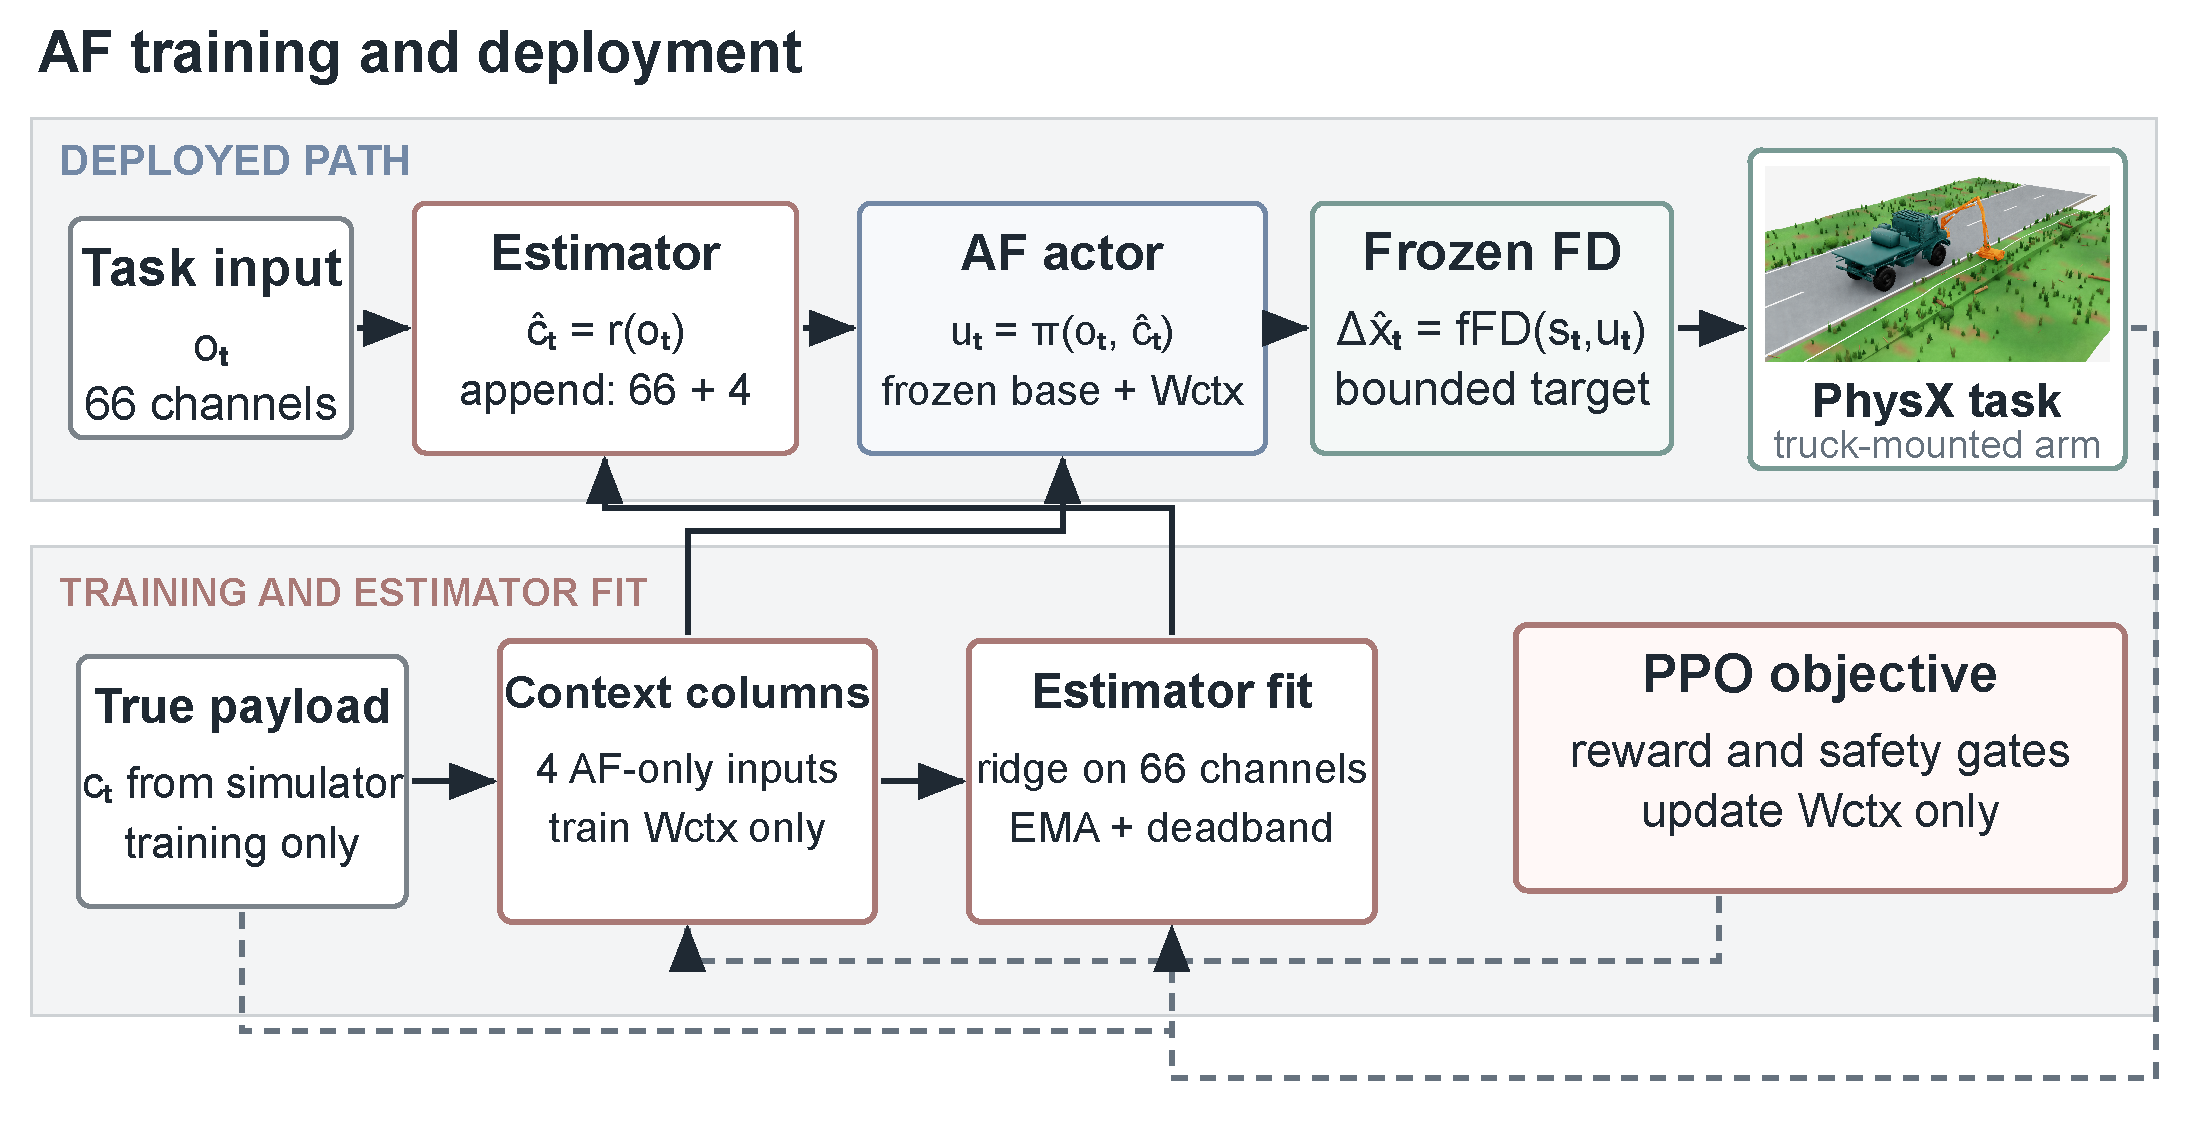
\includegraphics[width=1.08\textwidth]{images/ch6/ch6_aam_stack}}
  \caption{AF training and deployment. A ridge estimator maps the $66$-channel
  task input to four AF-only context values, applies EMA and a deadband, and
  appends them to the actor input. The actor combines its frozen base with
  $\bm{W}_{\mathrm{ctx}}$ and sends valve commands through Frozen FD to PhysX.
  During training, true payload supplies the context inputs and PPO updates only
  the $1\,024$ weights of $\bm{W}_{\mathrm{ctx}}$; the estimator is fitted
  afterwards on trained-policy rollouts. Dashed paths show updates and fitting
  data.}
\label{fig:ctrl:aam-stack}
\end{figure}

\begin{figure}[!htbp]
  \centering
  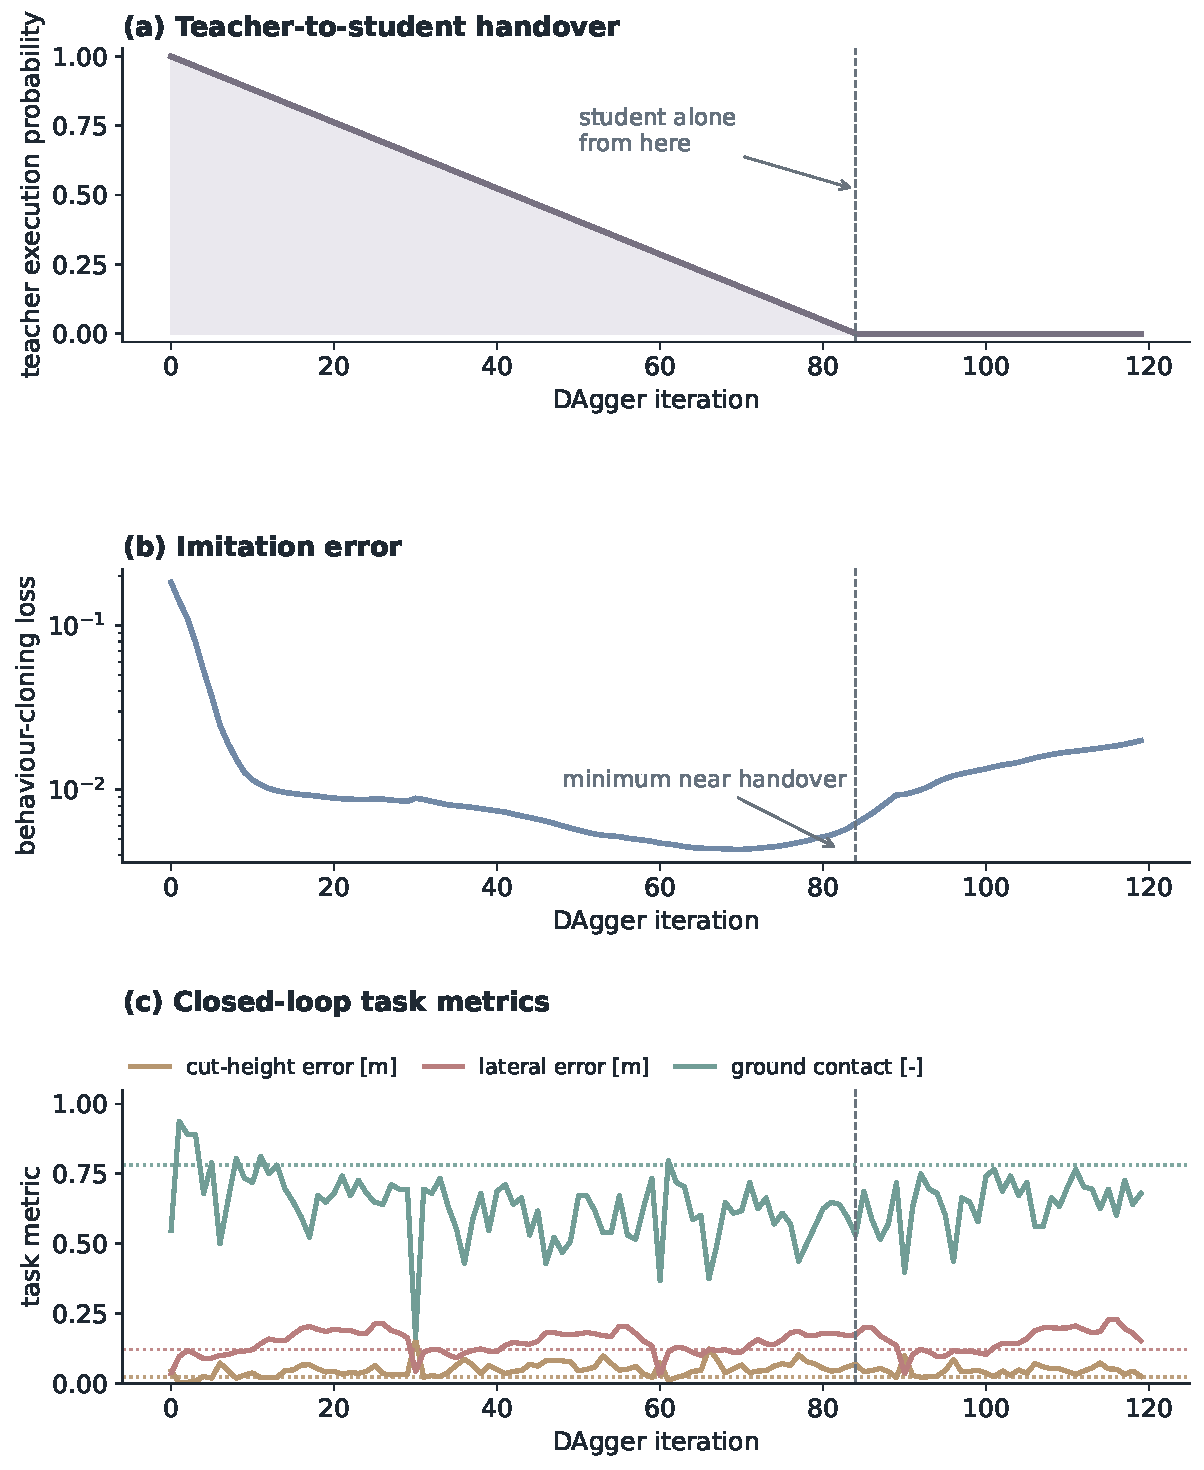
\includegraphics[width=\textwidth]{images/ch6/ch6_distillation}
  \caption{A measured distillation run for the \ppoROM{} stack. (a)~The
  teacher's execution probability falls to zero over the first $70\,\%$ of
  iterations. (b)~Behaviour-cloning loss falls by over an order of magnitude
  under teacher execution, then rises as the student visits new states.
  (c)~Cut-height error, lateral error and ground-contact fraction; dotted lines
  mark the teacher's preflight values from Table~\ref{tab:ctrl:teacher}.}
  \label{fig:ctrl:distillation}
\end{figure}


\subsection{Omission of the Inverse Model}
\label{sec:ctrl:af-no-id}

The inverse model belongs in \ppoIDFD{} and not in the adaptive stack, and the
reason is the same measurement in both cases. \ppoIDFD{} prices the cost of
substituting an independently identified pair for the deployment plant, and that
question needs the inverse model: a policy commanding desired cylinder motion
needs a map from intent to valve command, and supplying that map from
identification data alone is the substitution being priced.

Adaptation needs something the same map cannot give. Because the model predicts
a valve-command \emph{increment} that is accumulated and clipped
(Section~\ref{sec:models:id}), sustained demand walks the command onto its limit
and holds it there. Fed its own predictions the composite left the reference in
every one of the $118$ runs, with the pre-clip command at its limit on
$89.1\,\%$ of elements while the ROM valve on the same runs never reached its
bound. Closed-loop instrumentation over the $33$-cell panel says the same thing
in adaptation's terms: the command sat at its pre-clip limit on $79.9\,\%$ of
valve elements, $34.5\,\%$ of computed corrections were clipped away, and on
$37.9\,\%$ of elements the correction could not move the command at all.

The quantity being adapted and the quantity being saturated are therefore the
same, which makes a null through that path uninterpretable: it cannot separate a
task that is not adaptation-limited from credit clipped before it reached the
metric. Nothing here retracts what is claimed for \ppoIDFD{}, where the command
is consumed as issued. The final stack emits the valve command directly, so the
conditioning acts on the same bounded command as the policy.

\subsection{Sufficiency of the Forward Model}
\label{sec:ctrl:af-fd-sufficient}

Removing one of the two learned models raises the question of whether the
remaining one carries the path. The claim is specific: the forward model must
convert a commanded valve position into a one-step extension increment with
genuine valve sensitivity, because that increment is the only quantity the
controller integrates. The evidence is the strict retraining of
Section~\ref{sec:models:fd-identifiability}, which raises the valve-zero error
ratio from $0.94$ to $1.81$.

Sufficiency is established on the channel that is used and is not claimed beyond
it. Three qualifications carry forward. Only the extension increment is
integrated, the velocity output remaining weak on two axes and retained as a
diagnostic. Zero-order hold remains competitive below $\unit[0.25]{s}$, so the
forward model earns its place at the horizons the controller actually spans
rather than uniformly. And the valve authority the model represents is strongly
operating-point dependent, varying by a factor of $15$--$75$ across pressure
quartiles and capable of changing sign, which is why a constant valve Jacobian
was rejected.

\subsection{Conditioning on the Payload Estimate}
\label{sec:ctrl:af-residual}

Adaptation enters through the actor input rather than through its output. The
$66$-value observation is extended by four normalised plant-context channels,
and the actor's first layer is widened to receive them:
%
\begin{equation}
  \label{eq:ctrl:af-residual}
  \bm{u} = \pi_{\mathrm{frozen}}\bigl( \bm{o},\, \hat{\bm{c}} \bigr)
  = \operatorname{base}(\bm{o}) + \bm{W}_{\mathrm{ctx}} \hat{\bm{c}} ,
  \qquad
  \hat{\bm{c}} = \bm{0} \;\Rightarrow\; \bm{u} = \operatorname{base}(\bm{o}) .
\end{equation}
%
Only $\bm{W}_{\mathrm{ctx}}$ is trained: $1\,024$ parameters against a
$59\,588$-parameter frozen base, with the input-layer gradient masked to the
four context columns and every other parameter left untouched.

The identity on the right is what makes the comparison exact rather than
approximate. Nominal is the zero vector, so the frozen arm is not a separately
trained control but the same network evaluated at $\hat{\bm{c}} = \bm{0}$, and
it is recovered bit for bit. The base task columns are verified identical across
training seeds after adaptation training, which confirms the mask held.

The payload channel is normalised as $(m - 1)/0.5$, so a nominal cutter maps to
zero and a fivefold payload to eight. The estimate itself is not learned end to
end. It is a ridge regression on the $66$ task channels, fitted offline on
rollouts of the policy it will serve, then applied at runtime and smoothed by an
exponential moving average that is reset to nominal at every episode boundary.
A deadband holds the estimate at exactly nominal until the evidence is strong
enough to leave it, so on a plant that does not need the correction the deployed
controller is the frozen one.

\subsection{Freezing the Base Policy}
\label{sec:ctrl:af-frozen}

The base is frozen because anchored fine-tuning suppresses new context
dependence, while removing the anchor lets PPO trade line tracking for ground
contact. Even a $1000$-fold gradient multiplier moved action sensitivity only
from $0.001\,\%$ to $0.004\,\%$ of scale over $400$ iterations; masking the
anchor reached $0.005\,\%$. Training the context columns against a frozen base
avoids that suppression entirely, since the anchor never applies to them.

\subsection{Training of the Context Columns}
\label{sec:ctrl:af-encoder}

The context columns are trained under the reinforcement objective on the true
payload, and the estimator that replaces it at deployment is fitted afterwards
on rollouts of the trained policy. Separating the two matters: the regression
is on the observation distribution that policy induces, so an estimator fitted
from one policy does not transfer to another, and each training seed receives
its own fit. Nothing constrains which of the four context channels the policy
uses. Chapter~\ref{chap:evaluation} reports which it selects.

\subsection{Consistency With the Plant Dynamics}
\label{sec:ctrl:af-consistency}

Two consistency requirements follow from the system model of
Chapter~\ref{chap:system}, and both are met by construction.

The first is causality. The estimate is formed from the $66$-value policy
observation alone, every channel of which the deployed stack already produces at
runtime. The privileged factor vector, the true payload and any hidden simulator
state are excluded, so nothing enters the deployed path that would be
unavailable on the physical machine. The estimate also starts each episode at
nominal, which is the sense in which the machine works out what it is carrying
while driving rather than being told.

The task reference is not excluded, so the regression could in principle read
terrain and task state rather than load.
Section~\ref{sec:eval:attribution} tests that directly by permuting the payload
across environments, which leaves the distribution of the context untouched and
destroys only its correspondence to the plant it describes.

The pressure differences among those channels are recursive states of the frozen
forward model rather than plant measurements. The estimate is therefore faithful
only to the extent bounded in Section~\ref{sec:ctrl:af-fd-sufficient}, and
carrying it to the physical FME~500 would need differential-pressure
instrumentation the machine does not have. Every result here uses the
pressure-inclusive observation row; a strictly deployable row excluding measured
pressure is defined but not scored.

\subsection{Scope of the Claims}
\label{sec:ctrl:af-claims}

The smoothing rate of the estimate is a tuned hyperparameter, and its effect is
not neutral: the gradual arrival of the estimate is part of the mechanism rather
than an implementation detail, to the point that supplying the true payload
immediately is not an upper bound on what the estimate achieves
(Section~\ref{sec:eval:adaptation}).
The adaptation claim is made inside \ppoAAMFD{}, on the identified forward
model: frozen base, online estimate, and true payload. Chapter~\ref{chap:evaluation}
separates architecture-level evidence that the conditioning can reach the plant
from method-level evidence about whether the improvement replicates across
training seeds, and reports the payload regime in which it holds.

\section{IsaacLab Integration and Timing}
\label{sec:ctrl:integration}

Table~\ref{tab:app:rates} lists the concurrent rates: PhysX integrates at
$\unit[120]{Hz}$, the policy and its payload estimate run at $\unit[60]{Hz}$, and the
learned actuator models advance at $\unit[20]{Hz}$. No single value describes
the whole control loop.

The relationship between the $\unit[60]{Hz}$ and $\unit[20]{Hz}$ layers is where
integration errors hide, so it is fixed by construction rather than by
interpolation. A learned actuator model is evaluated on every third control step
and its predicted increment is held across the two intervening steps. The action
presented to the model is the action of the tick on which it fires, not an
average, and the target integrator accumulates in reference space, because
integrating against the measured extension turns a static hold into a slow
ratchet (Chapter~\ref{chap:system}).

Within each tick, the encoder consumes history ending at the previous tick before
the actuator path runs. Per-environment buffers are cleared on asynchronous
resets. A trace replay checks bit-exact agreement with an offline causal
recomputation, and checkpoint loading rejects mismatched normalisation,
features or history length.

\section{Constraints and Fair-Comparison Rules}
\label{sec:ctrl:constraints}

\subsection{Limits and Safeguards}

Authority is bounded by the action-chain rate, travel shield and lead cap, then
by per-axis valve limits. The environment terminates on the safety conditions of
Section~\ref{sec:sys:evaluation-criteria}, and every learned component has a
defined fallback for non-finite output.

Preflight also asserts that each reference remains within the measured
$\unit[0.240]{m/s}$ lateral authority ceiling of
Section~\ref{sec:sys:capability}; a faster path would be infeasible regardless of
the reward or optimiser.

\subsection{Matching Rules and Comparison Controls}
\label{sec:ctrl:matching}

Two comparisons carry distinct claims; the thesis does not rank all three
stacks.

\paragraph{The Matched Pair: R Against IF}
The representation claim rests on \ppoROM{} and \ppoIDFD, which differ only in
the actuator path. Their task, paths, terrain and held-out meshes, reward,
action bounds, gates, episode length, networks and training construction are
identical. Only this pair supports an across-stack comparison.

One departure is declared. Because the command ROM plus PhysX \emph{is} the
deployment plant (Section~\ref{sec:models:rom-calibration}), \ppoROM's tracking
advantage over \ppoIDFD{} is not evidence that a reduced-order model
approximates the actuator better than an identified pair: one of the two defines
the target.

\paragraph{The Paired Comparison: AF Against Its Own Frozen Base}
The adaptation claim is made within AF. Its arms share the frozen base,
training budget, reward and evaluation conditions, and are the same network
evaluated at different context values (Section~\ref{sec:ctrl:af-residual}).
Estimated, zeroed and permuted context are compared within seed and paired
environment by environment. The
primary checkpoint rule uses training reward without consulting held-out
performance; the fixed final checkpoint provides a robustness analysis
(Sections~\ref{sec:eval:attribution} and~\ref{sec:eval:adaptation}).

\paragraph{Fine-Tuning Budgets Must Be Matched or Reported}
Because reward ascent can move a policy away from the evaluation criterion
(Section~\ref{sec:ctrl:finding}), fine-tuning budgets must be matched or reported
as an additional treatment. The paired AF construction satisfies this rule.

\RRLABchapterblank
\chapter{Experimental Evaluation and Discussion}
\label{chap:evaluation}

This chapter evaluates the closed-loop stacks defined in
Chapter~\ref{chap:control}. The assessment has two parts.
Sections~\ref{sec:eval:tracking}--\ref{sec:eval:robustness} compare the matched
stacks \ppoROM{} and \ppoIDFD{}, which differ only in the actuator
representation. Section~\ref{sec:eval:adaptation} examines online adaptation
inside \ppoAAMFD{}, where the action contract is different and only within-stack
comparisons are valid. Section~\ref{sec:eval:discussion} draws the two parts
together.

The first part concerns tracking, command behaviour, response time, and
robustness under the reserved plant configurations. The second part concerns
whether a history-conditioned residual improves on a frozen base when cutter
mass changes during the episode.

\section{Experimental Protocol}
\label{sec:eval:hypotheses}

\subsection{Test Conditions and Comparisons}
\label{sec:eval:matrix}

All closed-loop results use held-out terrain meshes, eleven trajectory families,
a truck speed of \unit[4]{km/h}, a \unit[26]{m} scoring window, and sixteen
reserved plant configurations. The matched comparison is between \ppoROM{} and
\ppoIDFD{}. These stacks share the training configuration and differ in the
actuator representation. Adaptation is assessed only inside \ppoAAMFD{}, by
comparing a frozen base policy, a capacity-matched residual without history,
and a history-conditioned residual.

The results are paired by environment or by mesh and trajectory family. Error
metrics are reported separately for lateral tracking and cut height because the
two errors describe different aspects of the task. Confidence intervals are
obtained by paired bootstrap. Checkpoints are selected using the validation or
training criterion specified for each experiment and are then evaluated once on
the held-out set.

\subsection{Comparative Scope and Scoring}
\label{sec:eval:standing}

\ppoROM{} and \ppoIDFD{} form the cross-stack comparison. \ppoAAMFD{} has a
different action contract and is therefore not ranked against that pair. Its
results are interpreted only through within-stack comparisons.

\subsection{Scoring Horizon}
\label{sec:eval:horizon}

All reported closed-loop results use the full \unit[26]{m} trajectory rather
than a shorter selection window.

\section{Closed-Loop Task Performance}
\label{sec:eval:tracking}

The first comparison reports closed-loop tracking of \ppoROM{} and \ppoIDFD{}
on the held-out meshes and trajectory families.

The task is scored on two independent error channels, drawn side by side in
Figure~\ref{fig:eval:paths}: lateral error is deviation from the planned
cutting line in the horizontal plane, and cut-height error is deviation from the
intended vertical cut. They are kept separate throughout because a controller
can improve one while worsening the other. Ground contact, impacts and tool
acceleration are reported alongside them as checks on motion quality.

\begin{figure}[tbp]
  \centering
  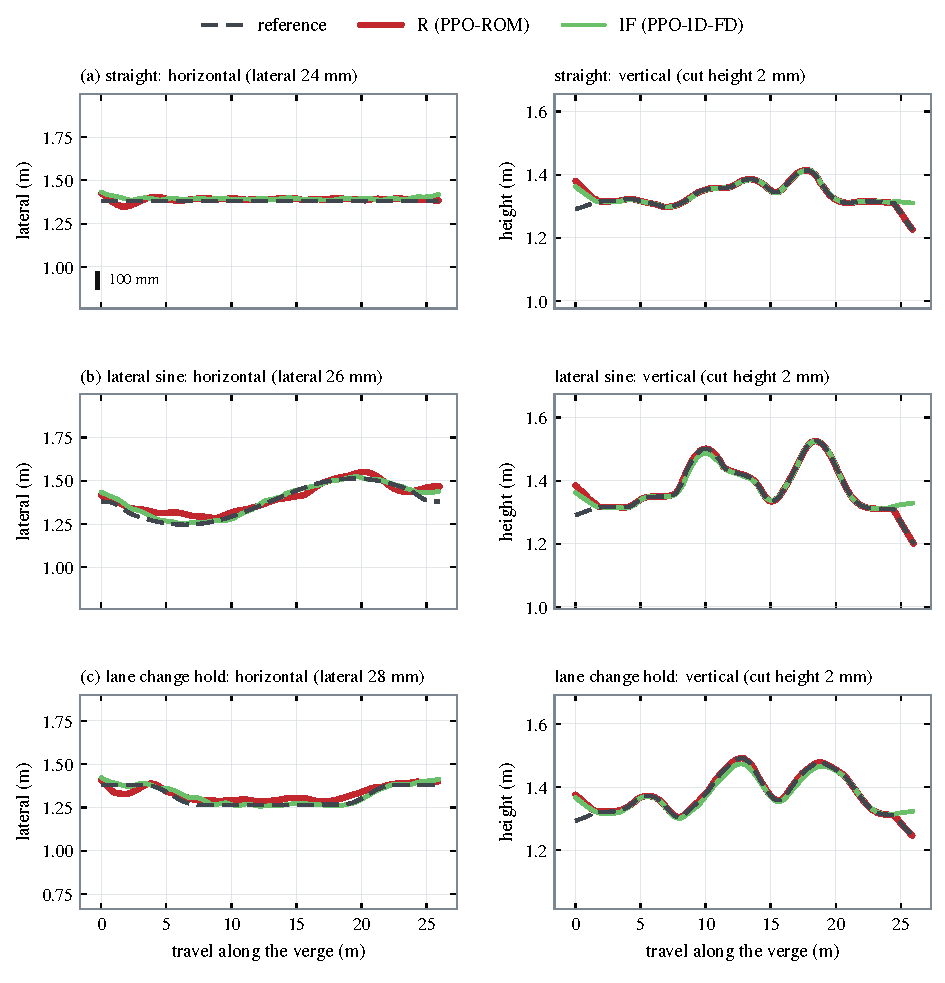
\includegraphics[width=\textwidth]{images/ch7/ch7_e1_paths}
  \caption{Cutter path against the reference on held-out mesh $1337$, for three
  structurally different trajectory families: a flat line, a smooth periodic
  sweep and a step-and-hold. The left column is the horizontal plane and the
  right column the vertical plane over the same drive. The vertical reference is
  not recorded directly and is recovered as
  $z_{\mathrm{ref}} = z_{\mathrm{cutter}} - e_{\mathrm{cut}}$, so both columns
  compare reference against actual. In the vertical panels the reference is
  largely hidden beneath both traces, which is what a millimetre-scale
  cut-height error looks like drawn at path scale.}
  \label{fig:eval:paths}
\end{figure}

Table~\ref{tab:eval:tracking} compares the matched pair over $33$ held-out
(mesh, family) conditions. Median errors are low for both stacks, and the p95
values move in the same direction as the means, so the improvement also reduces
the larger tracking deviations rather than only the average.

\begin{table}[tbp]
  \centering
  \caption{Closed-loop performance over $33$ paired held-out conditions. The
  matched stacks differ only in the actuator representation.}
  \label{tab:eval:tracking}
  \begin{tabular}{lcc}
    \toprule
    & \ppoROM{} & \ppoIDFD{} \\
    \midrule
    lateral error, mean (m) & $0.1026$ & $\mathbf{0.0703}$ \\
    lateral error, median (m) & $0.0392$ & $\mathbf{0.0281}$ \\
    lateral error, p95 (m) & $0.4664$ & $\mathbf{0.2665}$ \\
    cut-height error, mean (m) & $0.0084$ & $\mathbf{0.0063}$ \\
    cut-height error, median (m) & $\mathbf{0.0013}$ & $0.0031$ \\
    ground contact & $\mathbf{0.9623}$ & $0.9529$ \\
    hard impacts & $0.0947$ & $\mathbf{0.0905}$ \\
    tool acceleration p95 (m/s$^2$) & $39.90$ & $\mathbf{39.02}$ \\
    \bottomrule
  \end{tabular}
\end{table}

\begin{figure}[tbp]
  \centering
  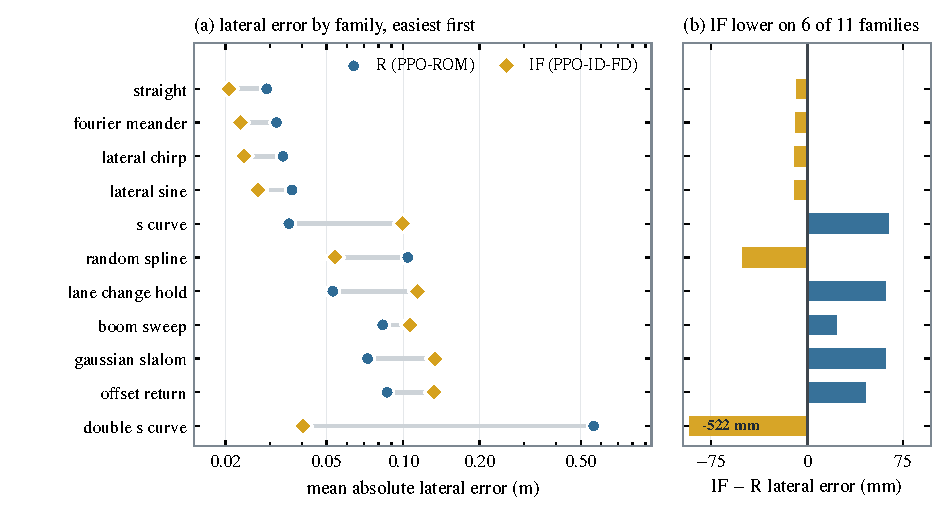
\includegraphics[width=\textwidth]{images/ch7/ch7_e1_tracking}
  \caption{Lateral error by trajectory family for the matched pair. The
  aggregate difference is concentrated in the more difficult families.}
  \label{fig:eval:tracking}
\end{figure}

Figure~\ref{fig:eval:tracking} resolves the aggregate by trajectory family.
\ppoIDFD{} reduces mean lateral error from \unit[0.103]{m} to \unit[0.070]{m}
and mean cut-height error from \unit[8.4]{mm} to \unit[6.3]{mm} over the $33$
paired conditions. The advantage is not uniform: \ppoIDFD{} is better on six of
the eleven families and \ppoROM{} on five, with the largest difference on the
double S-curve. The difference is concentrated on the more demanding families.
Both stacks follow the simpler paths closely.

\section{Actuator Representation and Dynamic Response}
\label{sec:eval:delay}

The same matched pair is now examined in the actuation channel: transport
delay, closed-loop step response, and command effort.

\subsection{Plant Delay and Step Response}
\label{sec:eval:delay-plant}

Open-loop excitation measured a command-to-pressure delay of approximately
\unit[117]{ms}. Cylinder extension and joint motion began at the same time,
which confirms that the dominant delay is hydraulic rather than kinematic. The
similar values across excitation amplitudes indicate that this delay is a stable
property of the simulated actuation chain.

\begin{table}[tbp]
  \centering
  \caption{Transport latency along the actuation chain, in milliseconds.
  Values are medians over open-loop excitation runs at \unit[60]{Hz}.}
  \label{tab:eval:delay}
  \begin{tabular}{lcccc}
    \toprule
    & \multicolumn{4}{c}{excitation amplitude} \\
    \cmidrule(lr){2-5}
    Link & $0.05$ & $0.15$ & $0.35$ & $0.70$ \\
    \midrule
    command $\rightarrow$ differential pressure & $117$ & $117$ & $117$ & $150$ \\
    command $\rightarrow$ cylinder velocity & $183$ & $167$ & $133$ & $117$ \\
    command $\rightarrow$ cylinder extension & $117$ & $117$ & $100$ & $100$ \\
    command $\rightarrow$ joint position & $117$ & $117$ & $100$ & $100$ \\
    \bottomrule
  \end{tabular}
\end{table}

The commanded-step experiment measures the closed-loop response to a
\unit[100]{mm} change in the reference line. Rise time is measured from
$10$ to $90\,\%$ of the step. Settling time is the first point at which the
error remains within \unit[20]{mm} for \unit[0.5]{s}.
\label{sec:eval:step-response}

\begin{table}[tbp]
  \centering
  \caption{Response to a \unit[100]{mm} commanded step. Values are median
  times over sixteen environments.}
  \label{tab:eval:step}
  \begin{tabular}{lcccc}
    \toprule
    Stack & detected response & rise & settled & overshoot \\
    \midrule
    \ppoROM{} & $333$ & $617$ & $2633$ & $57\,\%$ \\
    \ppoIDFD{} & $350$ & $717$ & $2183$ & $73\,\%$ \\
    \bottomrule
  \end{tabular}
  \\[2pt]
  \footnotesize Times are in milliseconds.
\end{table}

\ppoIDFD{} settles about \unit[0.45]{s} earlier, whereas \ppoROM{} has lower
overshoot. The command rate limit alone requires at least \unit[417]{ms} to
complete this step, and both stacks require more than \unit[2]{s} to settle.
Reducing hydraulic delay alone would therefore not remove the observed settling
time; the command rate, the policy response and the reference handling would
have to change with it.

Closed-loop settling is much slower than the hydraulic delay. Command-rate
limits and policy dynamics dominate the response time. The actuator path changes
the shape of the step, not the main settling time.

\subsection{Control Effort}
\label{sec:eval:effort}

\begin{table}[tbp]
  \centering
  \caption{Control effort on a held-out mesh. Lateral error is in millimetres;
  commands are in normalised units.}
  \label{tab:eval:effort}
  \begin{tabular}{lcccc}
    \toprule
    Stack & RMS command & rate RMS & reversals/s & lateral error \\
    \midrule
    \ppoROM{} & $0.586$ & $7.55$ & $40.0$ & $120.1$ \\
    \ppoIDFD{} & $0.827$ & $10.68$ & $\mathbf{10.6}$ & $\mathbf{26.8}$ \\
    \bottomrule
  \end{tabular}
\end{table}

\begin{figure}[tbp]
  \centering
  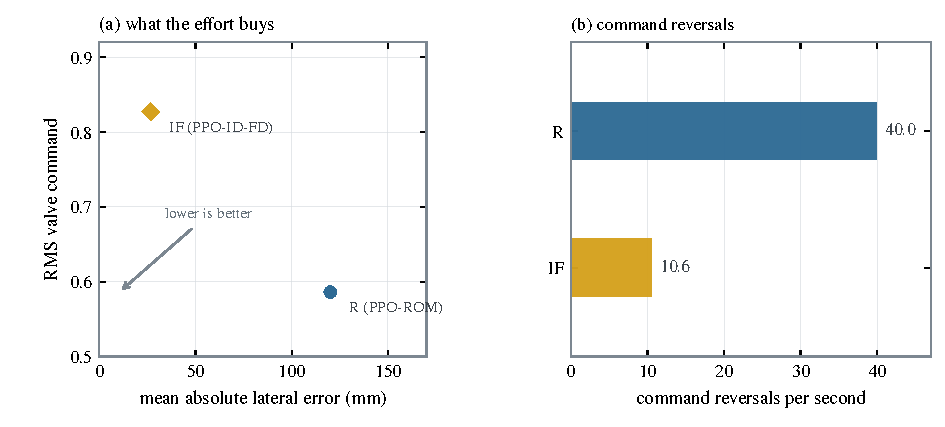
\includegraphics[width=\textwidth]{images/ch7/ch7_control_effort}
  \caption{(a) Control effort against the tracking error it buys for the matched
  pair; the lower left is better. (b) Command reversals per second, which the
  root-mean-square command does not reveal.}
  \label{fig:eval:effort}
\end{figure}

The reversal count identifies rapid changes in command direction that the
root-mean-square magnitude does not reveal, and
Figure~\ref{fig:eval:effort} pairs each stack's effort with the tracking error
it buys. A lower RMS command is not preferable when it comes with frequent
reversals and larger path error.

\ppoROM{} uses a smaller command magnitude but reverses almost four times as
often. \ppoIDFD{} uses more actuation, reverses less, and tracks more closely.
Effort is therefore reported together with the tracking it buys.

\section{Generalisation and Robustness}
\label{sec:eval:robustness}

The preceding sections use the held-out evaluation set. This section records
what that set does and does not establish, and then applies a common authority
reduction to all stacks.

The matched stacks generalise to the held-out meshes, trajectory families, and
reserved plant configurations used in this chapter. The randomisation sweep
showed little change in tracking over the tested mechanical variation. Its
hydraulic interpretation is limited because the inverse and forward plant does
not apply the hydraulic factors, while the reduced-order model constrains them
to its identification range.

The held-out evaluation therefore establishes transfer within the tested
simulation population. It does not establish performance on arbitrary hydraulic
conditions or physical hardware.

\subsection{Delivered Stress}
\label{sec:eval:delivered-stress}

The sweep therefore supports robustness to the tested changes in tool mass and
centre-of-mass height. It does not establish robustness to unbounded hydraulic
variation. A common authority perturbation was used to compare all stacks more
directly. This separates a reduction in realised actuator motion from the
specific randomisation factors used during deployment.

\subsection{Actuator Authority}
\label{sec:eval:boundary-design}

Actuator authority was reduced by scaling the realised actuator displacement:
\begin{equation}
  \label{eq:eval:authority}
  \Delta x^{\text{applied}}_k = \kappa\,\Delta x^{\text{actuator}}_k,
  \qquad \kappa \in (0,1].
\end{equation}

Here, $\kappa=1$ represents nominal authority and smaller values reduce the
motion delivered to the plant. The same perturbation is applied after each
stack's actuator representation, which makes the comparison independent of the
individual factor parameterisations.

\begin{figure}[tbp]
  \centering
  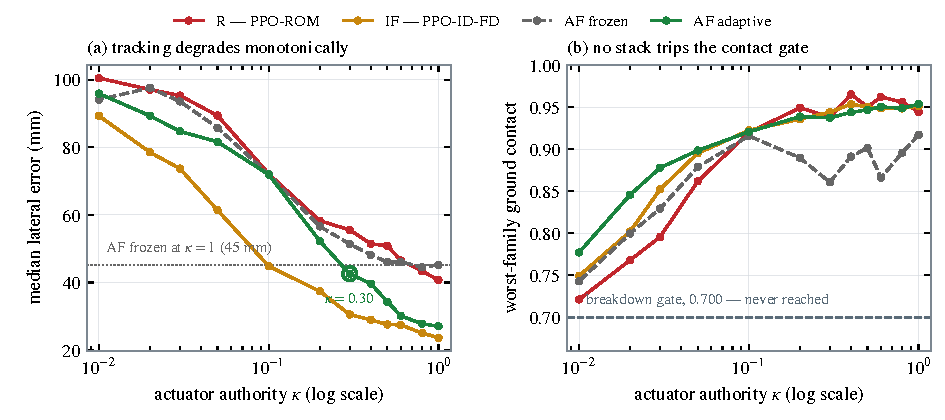
\includegraphics[width=\textwidth]{images/ch7/ch7_kappa_stacks}
  \caption{Lateral tracking and ground contact as actuator authority is reduced.
  The frozen and adaptive arms are compared within \ppoAAMFD{}.}
  \label{fig:eval:kappa-stacks}
\end{figure}

\begin{table}[tbp]
  \centering
  \caption{Authority at which median lateral error first reaches $1.5$ times
  its full-authority value.}
  \label{tab:eval:kappa}
  \begin{tabular}{lccc}
    \toprule
    Stack & nominal error (mm) & threshold (mm) & onset $\kappa$ \\
    \midrule
    \ppoROM{} & $40.69$ & $61.04$ & $0.10$ \\
    \ppoIDFD{} & $23.66$ & $35.49$ & $0.20$ \\
    \ppoAAMFD{} frozen & $45.18$ & $67.78$ & $0.10$ \\
    \ppoAAMFD{} adaptive & $27.03$ & $40.55$ & $0.30$ \\
    \bottomrule
  \end{tabular}
\end{table}

A hard robustness boundary was not observed over the tested authority range,
and \ppoIDFD{} had the lowest lateral error at every rung of the cross-stack
comparison.

No stack reached the contact or safety gate. Within \ppoAAMFD{}, the adaptive
residual holds the frozen residual's nominal lateral error down to
$\kappa=0.30$. This is an authority margin inside \ppoAAMFD{}. It is not a
ranking of \ppoAAMFD{} against \ppoROM{} or \ppoIDFD{}.

\section{Online Adaptation}
\label{sec:eval:adaptation}

The following experiments remain inside \ppoAAMFD{}. They test whether a
residual on the valve command improves on the frozen base when cutter mass
changes during the episode, and how much of any gain depends on live history
and on the size of the plant change.

\subsection{Experiment and Measurement}
\label{sec:eval:instrument}

The online-adaptation experiment changes cutter mass during each episode. The
change time and direction vary across environments. The three compared arms
share the frozen base policy, residual architecture, training budget, and
reward. The base has no residual, the control has a residual with a zeroed
history window, and the adaptive arm receives recent state-action history.

Changing mass during an episode creates a condition that cannot be addressed by
one fixed response. The varying change time prevents the residual from relying
on a fixed event schedule.

Results use $880$ paired environments across five held-out meshes. Lateral and
cut-height effects are evaluated separately. Cut-height effects smaller than
approximately $10\,\%$ are treated as unresolved because of the measurement
resolution; the corresponding lateral threshold is approximately $1.5\,\%$.
The paired design ensures that each arm is assessed under the same terrain,
trajectory, and mass-change condition.

\subsection{Performance Across Seeds}

\begin{table}[tbp]
  \centering
  \caption{History-conditioned residual against the frozen base over five
  training seeds. An asterisk indicates that the paired bootstrap interval
  excludes zero.}
  \label{tab:eval:arms}
  \begin{tabular}{lccc}
    \toprule
    Seed & cut-height gain & lateral gain & interpretation \\
    \midrule
    $17$ & $+39.1\,\%^{*}$ & $+84.9\,\%^{*}$ & improvement \\
    $23$ & $+35.5\,\%^{*}$ & $+4.0\,\%^{*}$ & improvement \\
    $101$ & $+74.7\,\%^{*}$ & $+5.9\,\%^{*}$ & improvement \\
    $42$ & $+43.4\,\%^{*}$ & $-16.1\,\%^{*}$ & trade-off \\
    $7$ & $+4.5\,\%$ & $+55.7\,\%^{*}$ & lateral improvement \\
    \bottomrule
  \end{tabular}
\end{table}

The percentages compare paired environments. A positive value means that the
adaptive arm has lower error than the frozen base for the median paired
environment. The bootstrap marker indicates that the paired difference is
resolved by the stated statistical test.

The adaptive residual improves at least one metric in four of five seeds. No
seed is worse on both metrics. The size of the effect varies, including a
trade-off on seed $42$, which is why the two error channels are not combined.

\subsection{Contribution of History}
\label{sec:eval:attribution}

The capacity-matched control separates the effect of the residual from the
effect of the history it receives.

\begin{table}[tbp]
  \centering
  \caption{Decomposition of the adaptive gain. The control and adaptive arms
  have the same capacity; only the adaptive arm receives live history.}
  \label{tab:eval:control-arm}
  \small
  \begin{tabular}{lcccc}
    \toprule
    & \multicolumn{2}{c}{base $\rightarrow$ control} & \multicolumn{2}{c}{control $\rightarrow$ adaptive} \\
    \cmidrule(lr){2-3}\cmidrule(lr){4-5}
    Seed & cut & lateral & cut & lateral \\
    \midrule
    $17$ & $+63.9\,\%^{*}$ & $-1.2\,\%$ & $-21.1\,\%^{*}$ & $+80.3\,\%^{*}$ \\
    $23$ & $+77.2\,\%^{*}$ & $+42.2\,\%^{*}$ & $-21.2\,\%^{*}$ & $-22.8\,\%^{*}$ \\
    $101$ & $+90.9\,\%^{*}$ & $+56.2\,\%^{*}$ & $-5.2\,\%$ & $-29.9\,\%^{*}$ \\
    $42$ & $+1.3\,\%$ & $-62.2\,\%^{*}$ & $+38.4\,\%^{*}$ & $+124.9\,\%^{*}$ \\
    $7$ & $+95.0\,\%^{*}$ & $+39.7\,\%^{*}$ & $-46.0\,\%^{*}$ & $+12.2\,\%^{*}$ \\
    \bottomrule
  \end{tabular}
\end{table}

This comparison is necessary because a larger residual can improve control even
when it receives no information about the current plant. The control arm has
the same trainable capacity and the same optimisation conditions as the adaptive
arm, so the difference between them is the live history and nothing else.

Residual capacity accounts for most of the cut-height gain in four seeds. The
additional effect of live history is mixed. The control arm is therefore not a
weaker adaptive arm; it isolates history from capacity.

\subsection{Plant-Dependent Contribution}
\label{sec:eval:dose}

To isolate plant-dependent adaptation, the mass-change magnitude was varied and
compared with a sham condition in which the event occurred without a change in
mass. The sham measures the benefit of the residual under the same event
schedule but without plant variation. The lateral benefit beyond the sham
increased with the mass change.

\begin{table}[tbp]
  \centering
  \caption{Lateral gain beyond the sham condition. Every interval excludes
  zero.}
  \label{tab:eval:dose}
  \begin{tabular}{lccc}
    \toprule
    Mass-change magnitude & total gain (mm) & gain beyond sham (mm) & interval (mm) \\
    \midrule
    $1.0$ (sham) & $16.557$ & n/a & n/a \\
    $1.5$ & $20.045$ & $3.796$ & $[2.303, 6.105]$ \\
    $2.0$ & $20.487$ & $3.912$ & $[1.693, 6.415]$ \\
    $2.5$ & $20.490$ & $4.073$ & $[2.318, 6.697]$ \\
    $3.0$ & $23.705$ & $7.410$ & $[4.785, 10.503]$ \\
    \bottomrule
  \end{tabular}
\end{table}

\begin{figure}[tbp]
  \centering
  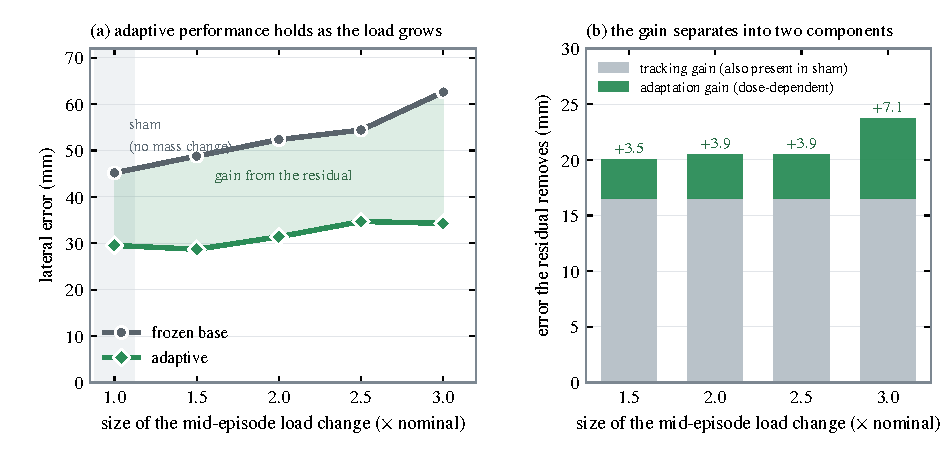
\includegraphics[width=\textwidth]{images/ch7/ch7_dose_response}
  \caption{Lateral performance across mass-change magnitudes. The sham
  condition separates general residual improvement from the contribution that
  increases with the plant change.}
  \label{fig:eval:dose}
\end{figure}

The trend is monotonic and resolved at every tested magnitude. The result is
limited to the perturbation and channel tested here: it does not show that
history conditioning improves every plant change or every task metric, only
that the lateral correction contains a measurable component that scales with
the mass change.

Lateral gain beyond the sham rises from \unit[3.8]{mm} at a $1.5$-fold mass
change to \unit[7.4]{mm} at a $3.0$-fold change. That component is
plant-dependent. It is about $31\,\%$ of the total lateral gain at the largest
change. The cut-height gain does not scale in the same way and is treated as a
general residual effect.

\subsection{The Pressure Channel Through the Load Change}
\label{sec:eval:pressure-signals}

The latent carries mainly seal condition
(Section~\ref{sec:models:aam-content}), and seal condition acts through
pressure, so the pressure the actuator model carries is where any conditioning
should first be visible. Figure~\ref{fig:eval:pressure-stacks} shows it per
cylinder for all three stacks, on the same plant and aligned on the same event.

\begin{figure}[tbp]
  \centering
  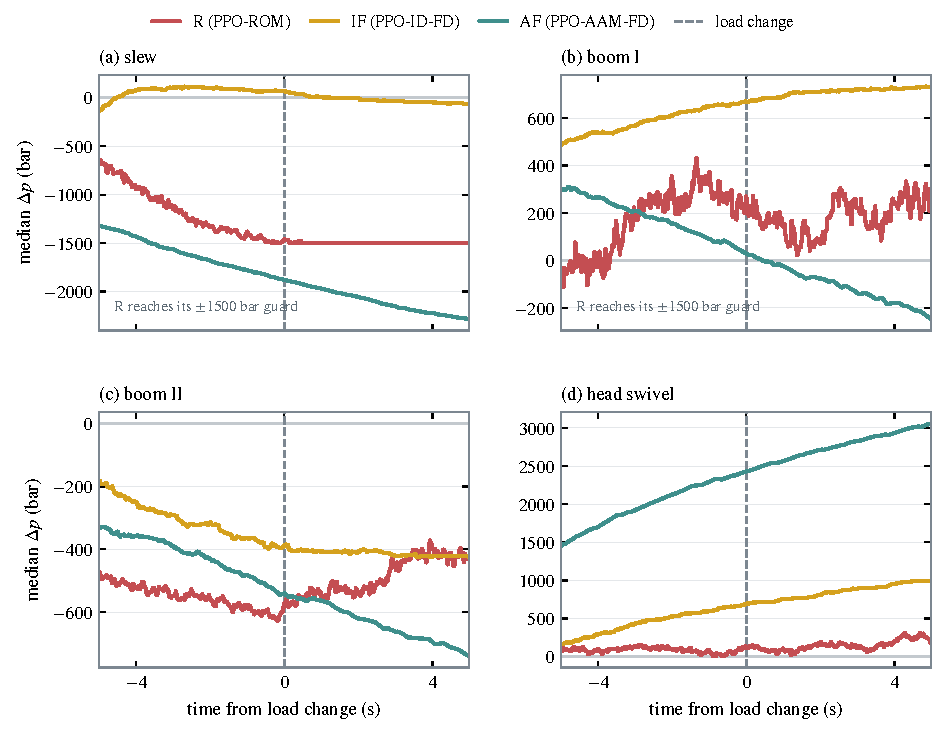
\includegraphics[width=\textwidth]{images/ch7/ch7_pressure_stacks}
  \caption{Median differential pressure per cylinder through the change of load,
  $151$ environments aligned on their own flip instant. The quantity is each
  stack's own actuator-model state, internal to the command ROM for \ppoROM{}
  and the forward model's recursive state for the other two, so the panels show
  what each controller believes about the hydraulics rather than a common
  measurement, and each panel carries its own scale. The slew and boom~I panels
  mark where \ppoROM{} sits on its \unit[1500]{bar} numerical guard.}
  \label{fig:eval:pressure-stacks}
\end{figure}

Two properties of the signal govern how the figure is read. The pressure state
is not a calibrated pressure on any stack: in this window the medians run to
\unit[2295]{bar} and the peaks to \unit[3784]{bar}, which is past what a
cylinder of this size could develop. The rod-force channel carries no supervised
weight and pressure-increment accuracy is only $R^2 = 0.06$ to $0.09$
(Section~\ref{sec:models:rom}). On \ppoROM{} the excursions are additionally
clipped by the \unit[1500]{bar} numerical guard, which binds on the slew and
the first boom cylinder and not on the other two. There is therefore no common
physical level the panels can be read against, and each cylinder is drawn on its
own scale. What the figure supports is the shape of the response either side of
the change, not the level.

Read that way, the traces are consistent with
Section~\ref{sec:eval:attribution}. Pressure state moves at the load change on
every stack, so the residual has access to a channel that reacts to the event.
The adaptive advantage is already present before the event, which is consistent
with continuous conditioning rather than a one-shot transient correction.

\section{Integrated Discussion}
\label{sec:eval:discussion}

\subsection*{Actuator Representation}

The inverse and forward actuator representation improved average tracking in
the matched comparison. It also reduced command reversals substantially.
Although the hydraulic transport delay was short, both stacks responded to a
reference step on a much longer time scale. Command limits and policy dynamics,
rather than the hydraulic delay, dominated closed-loop settling.

The tested stacks transferred to held-out terrain, trajectories, and plant
configurations. The authority experiment showed graceful degradation but did
not identify a hard safety boundary. Within \ppoAAMFD{}, the history-conditioned
residual retained the frozen residual's nominal tracking at lower actuator
authority. This is an authority-margin result, not evidence that it is the best
cross-stack controller.

\subsection*{Online Adaptation}

The history-conditioned residual improved on the frozen base in most training
seeds. The capacity-matched comparison shows that residual capacity explains a
large part of this result, so the overall gain cannot be assigned to history
alone. However, the sham-controlled dose experiment provides direct evidence
of a plant-dependent lateral contribution: the benefit increased with the size
of the mass change.

Online adaptation is therefore supported for the lateral channel under the
tested mass changes. Its contribution depends on plant variation reaching a
channel that the correction can influence and on the correction retaining
usable command authority. These conditions define the scope of the result.

\subsection*{Scope}

History-conditioned control has to be separated from added residual capacity. A
sham-controlled change is required to distinguish a general improvement from a
response that scales with the plant. For this manipulator, the measurable
plant-dependent benefit is limited to lateral tracking under the tested load
changes.

\RRLABchapterblank
%%%%%%%%%%%%%%%%%%%%%%%%%%%%%%%%%%%%%%%%%%%%%%%%%%%%%%%%%%%%
%% Chapter 8 - Conclusion and Future Work
%% Summarise what was established, answer the research questions,
%% identify next steps. No new experimental evidence.
%%%%%%%%%%%%%%%%%%%%%%%%%%%%%%%%%%%%%%%%%%%%%%%%%%%%%%%%%%%%
\chapter{Conclusion and Future Work}
\label{chap:conclusion}
\fancyhead[RE]{\headfont\nouppercase{\leftmark}}

This thesis asked how hydraulic actuator dynamics learned from high-fidelity
simulation can be reduced, transferred into a computationally efficient robotic
simulation and used for reinforcement-learning control, and under what
conditions online adaptation adds a further increment to the robustness those
learned models already provide. The six research questions of
Section~\ref{sec:intro:contributions} are answered in the order they were
asked, which is also the order in which the answers depend on one another.

\section{Summary of Findings}

The findings are stated in the order of the research questions. The first four
concern how hydraulic actuation is learned, transferred and controlled, and the
last two concern robustness and online adaptation. Figure~\ref{fig:concl:evidence-chain}
makes the dependency between those experiments explicit.

\begin{figure}[htbp]
  \centering
  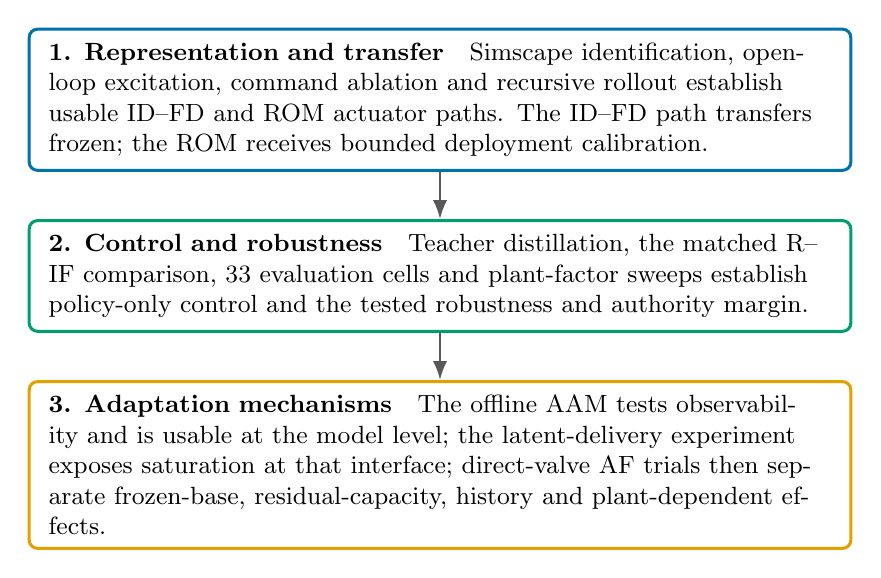
\begin{tikzpicture}[
    evidence/.style={draw=black!65, rounded corners=3pt, line width=.7pt,
      minimum height=14mm, text width=.82\textwidth, align=left,
      inner xsep=7pt, inner ysep=5pt, font=\small, fill=white},
    flow/.style={-{Latex[length=2.4mm]}, line width=.9pt, draw=black!65}
  ]
    \node[evidence, draw=cbblue, line width=1.1pt] (models) {\textbf{1. Representation and transfer}\quad
      Simscape identification, open-loop excitation, command ablation and
      recursive rollout establish usable ID--FD and ROM actuator paths. The
      ID--FD path transfers frozen; the ROM receives bounded deployment
      calibration.};
    \node[evidence, draw=cbgreen, line width=1.1pt, below=6mm of models] (control) {\textbf{2. Control and robustness}\quad
      Teacher distillation, the matched R--IF comparison, 33 evaluation cells
      and plant-factor sweeps establish policy-only control and the tested
      robustness and authority margin.};
    \node[evidence, draw=cborange, line width=1.1pt, below=6mm of control] (adapt) {\textbf{3. Adaptation mechanisms}\quad
      The offline AAM tests observability and is usable at the model level; the
      latent-delivery experiment exposes saturation at that interface; direct-valve
      AF trials then separate frozen-base, residual-capacity, history and
      plant-dependent effects.};
    \draw[flow] (models) -- (control);
    \draw[flow] (control) -- (adapt);
  \end{tikzpicture}
  \caption{Experimental evidence chain used to answer the research questions.
  Each stage constrains the claim made at the next stage; the final adaptation
  claim is interpreted only after transfer and robustness have been established.}
  \label{fig:concl:evidence-chain}
\end{figure}

\textbf{The inverse and forward representation identified in Simscape transfers
to the deployment simulation without retraining (RQ1, RQ2).} The inverse model
was trained on Simscape data alone and evaluated on all $118$ IsaacLab
deployment runs, drawn entirely outside that training distribution, where its
teacher-forced one-step extension error is millimetre-scale and nearly flat
across domains: $\unit[2.36]{mm}$ on the combined runs against $\unit[3.36]{mm}$
on nominal. The claim holds only in that one-step regime; closing the loop on
its own predictions diverges in all $118$ runs
(Section~\ref{sec:models:id-trust}). The reduced-order model received a small
bounded calibration against the deployment plant.

\textbf{Predictive accuracy must be accompanied by a control-authority test
(RQ1).} A learned actuator must be tested for dependence on the command, not
only for prediction error. With the accepted excitation design, removing the
valve input increases rollout error by a factor of $1.81$; before it, by $0.94$.
This is a general validation requirement for learned models used in control.

\textbf{Two actuator representations both support closed-loop control, and they
do not produce the same controller (RQ3, RQ5).} The command-conditioned
reduced-order model reaches $R^2 = 0.998$ on the internal valve state and $0.97$
on extension, and runs inside GPU-parallel training. The inverse--forward chain
composes two separately learned models in series, which could have compounded
their errors and did not. The two induce different control strategies from the
same policy interface. On the
recorded traces of one held-out mesh, \ppoROM{} spends the least command and
reverses about $40$ times per second against $10.6$ for \ppoIDFD{}, which
converts greater actuator effort into lower lateral error
(Table~\ref{tab:eval:effort}). Over the $33$ paired cells the median cell
favours \ppoIDFD{} on lateral error by $\unit[9.3]{mm}$ with the interval
excluding zero and favours \ppoROM{} on cut height by $\unit[1.7]{mm}$, while
neither mean difference is resolved and the mean changes sign if the double
S-curve family is removed (Table~\ref{tab:eval:paired-rif}). The choice of
representation therefore affects the resulting controller and is not an
implementation detail, but the size of that effect is not established.

\ppoROM{} and \ppoIDFD{} match on recorded training fields and differ only in
the actuator path. AF uses a different seed and training configuration and is
therefore evaluated through the paired within-stack comparison of
Section~\ref{sec:eval:attribution}, not ranked against them. With one R and one
IF training run, their seed variance remains unknown.

\textbf{A learned policy can replace the classical controller at runtime
(RQ4).} The damped-least-squares controller supplies privileged demonstrations
during training and is then removed; the distilled policy emits desired cylinder
motion directly into the learned actuator and is the entire deployed controller.
Over $33$ evaluation cells \ppoIDFD{} holds a mean lateral error of
$\unit[70.3]{mm}$, a median of $\unit[28.1]{mm}$ and $95.29\,\%$ ground contact
(Table~\ref{tab:eval:tracking}). The deployed policies remain anchored to the
demonstrated behaviour because the reward is an imperfect proxy for the
evaluation gates.

\textbf{The robust stacks retain a broad margin against mechanical variation
and authority loss without online adaptation (RQ2, RQ5).} On held-out meshes,
eleven trajectory families and sixteen reserved factor configurations,
\ppoIDFD{} meets the lateral criterion in $32$ of $33$ cells at a median of
$\unit[0.0281]{m}$. Its frozen inverse model transfers to all $118$ deployment
runs with millimetre-scale one-step error.

The factor sweep supports the tested mechanical variation, but not unbounded
hydraulic variation. On the inverse and forward path, hydraulic factors are not
applied; on \ppoROM{} they remain inside the identification range
(Section~\ref{sec:eval:delivered-stress}). Reducing realised actuator motion to
one per cent of nominal did not trigger the safety or ground-contact gates.
The result therefore establishes an authority margin, not a hard robustness
boundary (Section~\ref{sec:eval:boundary-design}).

\textbf{Online plant context is usable, and whether it reaches the closed loop
is set by the correction interface (RQ6).} The explicit mechanism estimates a
plant latent from recent interaction history. Its latent-conditioned adapters
beat a zero-context control on the adapter objective on all five seeds, and the
same correction changes no closed-loop metric, because it is added to an inverse
command already resting against its limit for most of the scored window. Moving
the correction onto the valve path restores the authority the residual needed.
At the pre-registered endpoint the history-conditioned residual succeeds on four
of five seeds; the fixed final checkpoint succeeds on three. An equal-capacity
zero-history residual also beats the frozen base on four seeds, so residual
capacity explains the median gain. Live history separates from that control on
one seed under each checkpoint rule. Restricting the encoder to plant-relevant
channels, the leading explanation for that absence, does not recover it: on a
plant where the frozen base degrades by two orders of magnitude across the mass
range, the primary comparison succeeds on two seeds of five and the median seed
fails (Section~\ref{sec:eval:starved}). Capacity alone beats the frozen base on
four of five there, one more than the history-conditioned arm. The cutter-mass study resolves a
load-dependent lateral component but compares against the frozen base, so it
cannot distinguish capacity from history. The supported method-level claim is
therefore the bounded residual; the history-specific increment is seed-dependent.

Table~\ref{tab:concl:adaptation-evidence} separates the experiments behind that
conclusion, so the gain of an enlarged residual is not read as evidence that
live history caused it.

\begin{table}[htbp]
  \centering
  \caption{Experimental decomposition of the adaptation claim. The rows answer
  different questions at different levels of the control chain and are not
  interchangeable evidence.}
  \label{tab:concl:adaptation-evidence}
  \small
  \setlength{\tabcolsep}{4pt}
  \begin{tabular}{@{}p{.20\textwidth}p{.27\textwidth}p{.43\textwidth}@{}}
    \toprule
    Experiment & Controlled comparison & Supported conclusion \\
    \midrule
    Latent adapter objective
      & estimated, privileged and zero latent on the adapter's own objective
      & Online plant context is usable at the model level: both latent arms beat the zero-context control on five of five seeds. \\
    Latent-delivery test
      & estimated, privileged and zero latent through the inverse-model correction path
      & Better plant context does not recover extension or velocity; saturation leaves insufficient correction authority at that interface. \\
    Primary seed table
      & history residual against its frozen base, paired within seed
      & The residual improves tracking on four of five seeds and the median seed passes; three of five at the final checkpoint. \\
    Capacity control
      & history-conditioned residual against an equal-capacity zero-history residual
      & Capacity alone reproduces most of that gain; live history separates from zeroed history on one seed of five at each checkpoint rule. \\
    Encoder restriction
      & history against zeroed history at equal capacity, encoder starved to plant-relevant channels
      & The missing history effect is not an artefact of a wide encoder input: two seeds of five succeed and the median seed fails. \\
    Cutter-mass dose and sham
      & plant perturbation against the corresponding sham condition
      & A plant-dependent lateral component is resolved, but starting mass and the later exchange remain coupled. \\
    \bottomrule
  \end{tabular}
\end{table}

\section{Design Implications}

The design implications follow the same sequence: actuator identification,
policy training and plant adaptation.

\subsection*{Identification and Transfer}

\textbf{Design the excitation for identifiability, and test the model by input
ablation.} Task-control data can make state and command nearly redundant.
Dedicated excitation makes command effects identifiable. A learned actuator
should therefore be accepted on both prediction accuracy and loss of performance
when the command input is removed.

\textbf{Embed known physics and bound learned corrections.} The reduced-order
model propagates pressure, force, velocity, and extension through explicit
updates. Its learned terms are bounded, preventing unphysical state changes
inside the training loop. This structure also represents the pressure dependence
of valve authority directly.

\textbf{Prefer a frozen model with a bounded, gated correction to retraining.}
The inverse model transferred at millimetre scale and remained frozen. A
$\unit[3]{mm}$ correction absorbed the deployment offset, vanished at zero
command and preserved the original data through replay, confining
deployment-specific behaviour to a bounded component.

\subsection*{Control Methodology}

\textbf{Constrain policy updates when the reward is not the evaluation
criterion.} The physical evaluation gates and the reward are not identical. A
forward-KL anchor to a verified reference policy bounds policy drift, and the
anchor advances only through checkpoints that satisfy the gates. Reward terms
should represent quantities that are also treated as evaluation constraints.

\textbf{Where no baseline is inherited, the action contract is the safety
argument.} Zero action leaves the arm stationary. A rate limit, filter, travel
shield, command scale and per-axis anti-windup cap bound its authority. The cap
must be resolved per axis because the value that recovers boom offsets damages
head alignment on cylinder~4 (Section~\ref{sec:ctrl:ppo}).

\subsection*{Plant Adaptation}

\textbf{Measure identifiability and correction authority before training an
estimator.} The identifiability envelope determines whether plant identity is
present in the data. The delivered-stress check determines whether a
perturbation reaches the plant and whether a correction can influence the
command. Both tests should precede estimator training.

Filtering may be needed when a changing estimate enters a memoryless policy,
but its time constant remains to be determined on the deployed stack.

\section{Contributions}

Section~\ref{sec:intro:contributions} stated six contributions. Their standing
at the end of the work is as follows, with the supporting evidence as summarised
above rather than repeated.

\textbf{Transferable hydraulic actuator learning} is delivered through two
Simscape-identified representations realised in IsaacLab; the inverse model
transfers without retraining. The \textbf{reduced-order actuator model} is a
bounded, differentiable surrogate suitable for GPU-parallel training and serves
as the calibrated deployment plant. Its clamped constants are not identified
physical parameters (Section~\ref{sec:models:rom}).

The \textbf{control-relevant identification and validation} procedure combines
input ablation, which exposed a forward model without command authority, with an
identifiability audit of the excitation envelope.

\textbf{Policy-only control through learned hydraulics} is demonstrated. After
the classical teacher is removed, \ppoIDFD{} holds a mean lateral error of
\unit[70]{mm} and a median of \unit[28]{mm} over $33$ held-out cells at
$95\,\%$ ground contact (Section~\ref{sec:eval:tracking}). Worst-cell
aggregation still misses two gates; that bound is stated in
Section~\ref{sec:concl:limitations}.

The \textbf{decision procedure for online adaptation} separates residual plant
sensitivity, observability, correction authority and residual capacity before
attributing a gain to adaptation. It also exposes when the optimiser trades away
a gated quantity that the reward does not price.

\textbf{Where online adaptation is effective} is answered at two levels. Plant
context is informative at the model level but cannot affect the saturated
inverse command. A bounded valve-path residual retains authority and improves
the median training run, although the capacity-matched control reproduces most
of the gain. Live history contributes only on seed-specific cases, and a second
campaign that starves the encoder to plant-relevant channels returns two of five
seeds, eliminating the encoder as the explanation. The cutter-mass study resolves
a plant-dependent lateral component without isolating the transient mass
exchange.

Two enablers are recorded: the causal estimator and bounded adaptation path use
no privileged or future information and revert safely on invalid input. Five of
the eight promotion gates separate the matched pair
(Section~\ref{sec:sys:gates}).

\section{Limitations}
\label{sec:concl:limitations}
\label{sec:conclusion:limitations}

\textbf{Scope of plant validation.} The evidence is simulation-to-simulation,
and the deployment plant is itself a learned model. No claim here is a claim
about hardware.

\textbf{Scope of hydraulic observability.} The differential pressure the estimator consumes is produced by the actuator
model rather than measured, so transferring the model-level result to hardware
requires instrumentation the FME~500 does not carry. An observation contract
remains unresolved alongside this: every result uses the pressure-inclusive row,
while the stricter deployable alternative excludes measured differential
pressure. Since the estimator's advantage is concentrated in that channel, the
deployable variant should be expected to perform worse, and by how much is not
established.

\textbf{Scope of controller comparison.} On worst-mesh, worst-family statistics
both stacks fail the lateral gate and \ppoIDFD{} does not satisfy the
head-alignment gate under worst-case aggregation
(Section~\ref{sec:eval:tracking}), so neither stack satisfies the whole
eight-gate evaluation contract. The closed-loop comparisons resolve differences to a few per cent over $33$
paired conditions and do not establish equivalence. The available plant
variation bounds the disturbance rather than the architecture, and more tightly
than the sweep's labels suggest. A stack has been shown to tolerate what
actually reached it, which on the inverse and forward plant is a mechanical
perturbation only, plus a generic reduction of realised actuator motion. Median
lateral error first reaches $1.5$ times its full-authority value at
$\kappa = 0.20$ for \ppoIDFD{} and $\kappa = 0.10$ for \ppoROM{}, and no stack
reaches the pre-declared breakdown gate down to $\kappa = 0.01$
(Section~\ref{sec:eval:boundary-design}). That is an authority margin, not a
demonstration of hydraulic robustness. The three
stacks are matched on evaluation but not on training budget, so the comparison
describes three deployed controllers rather than three equally tuned training
procedures.

\textbf{Scope of training variation.} Policy-training variation is not quantified for
the matched R and IF pair, and it bounds
two claims differently. R and IF are each represented by one training run, so
the $33$ paired cells measure terrain and trajectory variation and say nothing
about how far a second run of either would move; the actuator-representation
result rests on that assumption. The adaptation result includes five training
seeds and meets the primary criterion on four, so it establishes a median
improvement and not a uniform one. The defensible claim is an
architecture-level correction on the identified valve path, together with a
plant-dependent lateral term under the tested cutter-mass doses.

\textbf{Scope of the adaptation evidence.} The commanded step cannot finish faster than $417$\,ms at the command-rate limit,
while the plant answers in about $117$\,ms. That loop is a hard case for
adaptation understood as a reaction to a single event and favours continuous
conditioning on the operating point.
Appendix~\ref{app:pressure-signals} is consistent with the second reading:
the adaptive advantage is already present before the load change.
Section~\ref{sec:eval:dose} shows a cutter-mass-dependent lateral term relative
to the $1.0$ condition, which the coupled dose design does not resolve into a
transient adaptation response.

\section{Future Work}
\label{sec:concl:future}

The evidence in this thesis is simulation-to-simulation, and the three
experiments that would most change what it can claim are also in simulation.
They are listed first for that reason.

\textbf{Fit the encoder by regression rather than through the policy gradient.}
Restricting the encoder input has been done and did not recover the effect
(Section~\ref{sec:eval:starved}), which leaves the training signal rather than
the input width as the remaining candidate. Rapid motor adaptation never trains
its encoder through the policy gradient, fitting it onto a low-dimensional
privileged vector and freezing it before the residual head is
trained~\cite{kumar2021rma}. That is the one variant this campaign's
pre-registration admits, and it separates a representation problem from the
absence of a usable effect.

\textbf{Train more than one seed per representation.} R and IF are one training
run each, so the cross-stack comparison of Section~\ref{sec:eval:tracking}
describes two deployed controllers and cannot separate the representation from
the seed. Three or more runs per stack, scored on the same $33$ cells, would
convert that observation into a result at moderate cost.

\textbf{Ablate reference-anchored PPO.} Section~\ref{sec:ctrl:finding}
establishes that unconstrained fine-tuning fails; it does not establish that
this particular construction is what fixed it. A three-arm comparison against
plain PPO with early stopping and against the un-fine-tuned distilled policy
would separate the block ratchet from the constraint it sits inside.

\textbf{Then the machine.} Hardware evaluation begins by adding chamber-pressure
and extension sensing and a rod load pin to the FME~500. The open-loop excitation
schedule and identifiability audit of Chapter~\ref{chap:data} can then be applied
to machine data. Any correction should remain bounded, retain the identified
hydraulic parameters and original data for replay, and pass input ablation. The
reference-anchored policy provides the verified starting checkpoint.

The central design lesson is conditional. Robust training absorbs a large part
of the plant variation before online adaptation is introduced. A remaining
correction is useful only when the variation is observable, the fixed controller
leaves a deficit to recover, and the command path retains authority. Apparent
adaptation gains must also be separated from gains due to residual capacity.
Evaluating these conditions together provides a defensible basis for deciding
when online adaptation is justified on a hydraulic manipulator.

\RRLABchapterblank

%%%%%%%%%%%%%%%%%%%%%%%%%%%%%%%%%%%%%%%%%%%%%%%%%%%%%%%%%%%%
%% Appendices
%%%%%%%%%%%%%%%%%%%%%%%%%%%%%%%%%%%%%%%%%%%%%%%%%%%%%%%%%%%%
\appendix
%%%%%%%%%%%%%%%%%%%%%%%%%%%%%%%%%%%%%%%%%%%%%%%%%%%%%%%%%%%%
%% Focused appendices: only the reference data and the
%% reproduction record that the main chapters cannot carry.
%%%%%%%%%%%%%%%%%%%%%%%%%%%%%%%%%%%%%%%%%%%%%%%%%%%%%%%%%%%%

\chapter{Reference Data and Reproducibility Record}

This appendix retains only the reference numbers, digests and entry points that
the main chapters cannot carry.

\section{Plant Ranges and Frozen Collections}
\label{app:dataset}

\begin{table}[H]
  \centering
  \caption{Randomised parameters of the Simscape curriculum. Seal wear is drawn
  per cylinder and drives clearance, leakage and spool lag together; mechanical
  perturbations apply to each of the fourteen bodies.}
  \label{tab:data:hydraulic}
  \small
  \begin{tabular}{lll}
    \toprule
    Parameter & Nominal & Randomised range \\
    \midrule
    Entrained air fraction $\varepsilon_{\mathrm{air}}$
      & $0.005$ & $0.001$ -- $0.080$ \\
    Dead-volume fraction $\varepsilon_{\mathrm{vol}}$
      & $0.020$ & $0.005$ -- $0.080$ \\
    Discharge coefficient $c_d$
      & $0.70$ & $0.56$ -- $0.84$ \\
    Seal wear $w_{\mathrm{seal},i}$
      & $0$ & $0$ -- $0.25$ per cylinder \\
    Relief setting $p_{\mathrm{set}}$
      & $\unit[27.6]{MPa}$ & $\unit[24.8]{MPa}$ -- $\unit[30.4]{MPa}$ \\
    \midrule
    Body mass & CAD value & $\pm 20\,\%$ \\
    Centre-of-mass offset & CAD value & $\pm 5\,\%$ \\
    Inertia tensor & CAD value & consistent with mass draw \\
    Joint stiffness, J1--J4 & $\unit[60]{kN/m}$ & $40$ -- $\unit[120]{kN/m}$ \\
    Joint stiffness, J5 & $\unit[25]{kN/m}$ & $15$ -- $\unit[60]{kN/m}$ \\
    Joint damping & $250$ & $100$ -- $600$ \\
    \bottomrule
  \end{tabular}
\end{table}

\begin{table}[H]
  \centering
  \caption{Six physical factors in the IsaacLab deployment collections, one
  vector drawn per run and held fixed throughout it.}
  \label{tab:data:factors}
  \small
  \begin{tabular}{llll}
    \toprule
    Coordinate & Range & Domain & Acts on \\
    \midrule
    $e_{\mathrm{flow}}$       & $[-0.25,\, 0.25]$ & hydraulic  & valve flow gain \\
    $e_{\mathrm{compliance}}$ & $[-0.25,\, 0.10]$ & hydraulic  & effective chamber compliance \\
    $e_{\mathrm{seal}}$       & $[0,\, 1]$        & hydraulic  & seal wear, leakage, spool lag \\
    $e_{\mathrm{pressure}}$   & $[-0.15,\, 0.15]$ & hydraulic  & supply/relief pressure level \\
    $e_{\mathrm{mass}}$       & $[0.8,\, 1.5]$    & mechanical & cutter mass scale \\
    $e_{\mathrm{COM}_z}$      & $[-0.10,\, 0.05]$ & mechanical & cutter centre-of-mass height \\
    \bottomrule
  \end{tabular}
\end{table}

\label{app:data:frozen}
The task-controller and open-loop context-identification collections share the
same factor design and run-level split. Each contains $118$ runs with one fixed
factor vector per run: $64$ with all six factors varied, $40$ hydraulic-only,
$12$ mechanical-only and $2$ nominal, split into $82$ fitting, $20$ validation
and $16$ held-out test runs. Splitting is at run level, since the factor vector
is constant within a run and a window-level split would place near-duplicates of
the same plant in both sets; the manifests store the run identifier, factor key
and split label. Model-level identification results use the open-loop
collection for the reason given in
Section~\ref{sec:data:openloop-collection}.

\section{Timing Contract}

\begin{table}[H]
  \centering
  \caption{Rates of the simulation, control and learned components. The offline
  AAM is a diagnostic, not part of the deployed loop.}
  \label{tab:app:rates}
  \small
  \begin{tabular}{lll}
    \toprule
    Layer & Rate & Period \\
    \midrule
    PhysX physics substep           & $\unit[120]{Hz}$ & $\unit[8.33]{ms}$ \\
    Policy and control step         & $\unit[60]{Hz}$  & $\unit[16.67]{ms}$ \\
    AF payload estimate and context & $\unit[60]{Hz}$  & $\unit[16.67]{ms}$ \\
    Inverse, forward and ROM models & $\unit[20]{Hz}$  & $\unit[50]{ms}$ \\
    Offline AAM inference           & $\unit[20]{Hz}$  & $\unit[50]{ms}$ \\
    Simscape logging grid           & $\unit[20]{Hz}$  & $\unit[50]{ms}$ \\
    \bottomrule
  \end{tabular}
\end{table}

The offline AAM reads $20$ rows on the $\unit[20]{Hz}$ grid, a $\unit[1.0]{s}$
window, and its five-estimate smoother adds $\unit[250]{ms}$ of delay. Deployed
AF reads $20$ control-step rows, a $\unit[333]{ms}$ window, with no smoother.

\section{Frozen Artifacts}

\begin{table}[H]
  \centering
  \caption{Frozen artifacts and their SHA-256 digests, truncated to $32$
  hexadecimal digits. The context-column checkpoints share the frozen AF base
  and differ only in their $1\,024$ trained parameters.}
  \label{tab:app:hashes}
  \scriptsize
  \begin{tabular}{lll}
    \toprule
    Artifact & Role & SHA-256 (truncated) \\
    \midrule
    \texttt{aam.pt} & offline AAM & \texttt{cd6a7f0b118b96c7ce66b889b9b3e422} \\
    \texttt{zhat\_adapter.pt} & ID adapter & \texttt{30629a4f83db5c2bed3c777bcf82dc57} \\
    \texttt{best\_id\_cylinder\_control.pt} & inverse model & \texttt{8e26c52e82d89efe193e001d0a8b07a6} \\
    \texttt{best\_fd\_cylinder\_strict.pt} & forward model & \texttt{1f41e44309a8f320430a3382ca88ce5f} \\
    \midrule
    \texttt{rom\_s6\_aligned/model\_598.pt} & R policy & \texttt{ce7e3ab9649b1193f123f9f91107bbf8} \\
    \texttt{idfd\_s6\_aligned/model\_598.pt} & IF policy & \texttt{06533b8e8614b0ad982dd8c238a17772} \\
    \texttt{distilled\_v1/phase1\_init\_70.pt} & AF frozen base & \texttt{641e476cfcd765a8d68a17980d6cbbf2} \\
    \texttt{ctxonly17/model\_1596.pt} & AF context columns, seed $17$ & \texttt{805da12505d214ca9f40c405cf02e505} \\
    \texttt{ctxonly23/model\_1596.pt} & AF context columns, seed $23$ & \texttt{79778e16722bbf2ace1b5c0e680a47dd} \\
    \texttt{ctxonly101/model\_1596.pt} & AF context columns, seed $101$ & \texttt{80b15d39d0b61ed3ae5ac72b248d9329} \\
    \texttt{s17\_fit.npz} & payload estimator, seed $17$ & \texttt{1b48070e035f05b07f52449ee2a42b83} \\
    \texttt{s23\_fit.npz} & payload estimator, seed $23$ & \texttt{422a5f498b03426ab2fe26d52d724174} \\
    \texttt{s101\_fit.npz} & payload estimator, seed $101$ & \texttt{d7abd08b30d0489f8da593f3c5c0541e} \\
    \bottomrule
  \end{tabular}
\end{table}

\section{Derivation of the Reference-Divergence Gate Bound}
\label{app:kl-bound}

Let $P_\pi$ be the distribution over length-$H$ trajectories induced by $\pi$
under the fixed transition kernel. That kernel is shared by
$\pi_{\mathrm{ref}}$ and $\pi_\vartheta$, so it cancels from the log-ratio and
the chain rule of KL divergence~\cite{cover2006information} reduces the
trajectory divergence to a sum of $H$ per-step action divergences on
$\pi_{\mathrm{ref}}$'s own rollout distribution. Bounding each by the
training-time bound $\delta_{\mathrm{ref}}$ of
Equation~\eqref{eq:ctrl:bounds}, applying Pinsker's inequality and using
$\sum_\tau |P(\tau)-Q(\tau)| = 2\,\delta_{\mathrm{TV}}(P,Q)$ for a functional
$g$ with $\|g\|_\infty \le G_{\max}$ gives
%
\begin{equation}
  \bigl|\mathbb{E}_{\pi_\vartheta}[g] - \mathbb{E}_{\pi_{\mathrm{ref}}}[g]\bigr|
  \le 2\,G_{\max}\,
     \delta_{\mathrm{TV}}(P_{\pi_{\mathrm{ref}}}, P_{\pi_\vartheta})
  \le 2\,G_{\max}\sqrt{\tfrac{H\,\delta_{\mathrm{ref}}}{2}} .
  \label{eq:app:final-bound}
\end{equation}
%
At the production horizon $H = 2808$ and $\delta_{\mathrm{ref}} = 0.05$ the
right-hand side is $16.76$, which is vacuous for a gate metric normalised to
$[0,1]$. The chain-rule step is also exact only on states drawn from
$\pi_{\mathrm{ref}}$, whereas the training loop evaluates $D_{\mathrm{ref}}$ on
states the live policy visits. The construction is a principled restriction of
reward ascent to a neighbourhood of a verified policy, not a certificate.

\section{Reproduction Entry Points}
\label{app:repro}

\sloppypar
The closed-loop results of Chapter~\ref{chap:evaluation} are generated by the
scripts under \texttt{experiments/E1\_tracking\_and\_control\_effort} and \texttt{experiments/E2\_transport\_delay\_and\_identifiability}, each
recording its model, meshes, trajectory families, carrier speed and scored
horizon in a manifest. AF arms are trained and scored under
\texttt{PPO\_AAM\_FD/experiment\_scripts}, and the adaptation tables and figures
are recomputed from \texttt{outputs/final}, \texttt{outputs/heldout8191},
\texttt{outputs/aa\_floor} and \texttt{outputs/kappa\_loaded} by the scripts
there. Model-level results use the frozen collections of
Appendix~\ref{app:data:frozen}. Each pre-registered comparison also has a dated
design note under \texttt{reports/} fixing the success rule, checkpoint rule,
statistic and declared outcomes before its arms were trained; with the digests
of Table~\ref{tab:app:hashes} they identify the data, models, rules and code
behind every reported number.


%%%%%%%%%%%%%%%%%%%%%%%%%%%%%%%%%%%%%%%%%%%%%%%%%%%%%%%%%%%%
%% Bibliography
%%%%%%%%%%%%%%%%%%%%%%%%%%%%%%%%%%%%%%%%%%%%%%%%%%%%%%%%%%%%
\RRLABbibliography{literature}

\end{document}
